
\def\filedate{2011/05/20}\let\thedate\filedate % packages may change \filedate

\documentclass[11pt,twoside]{article}
\usepackage[obeyspaces]{url}
\usepackage{natbib}
\usepackage{chem}
\usepackage[usenames,dvipsnames,svgnames,table]{xcolor}
\usepackage{rotating} % loads graphicx
%\usepackage{longtable}
\usepackage{graphicx}
%\usepackage{verbatim}

\oddsidemargin-5mm
%\evensidemargin-15mm
\evensidemargin-5mm
\topmargin-10mm
\textheight230mm
\textwidth170mm
\raggedbottom
\parindent0mm
\parskip1.0ex plus0.5ex minus0.5ex
\renewcommand{\arraystretch}{1}
\renewcommand{\topfraction}{0.95}
\renewcommand{\dbltopfraction}{0.95}
\renewcommand{\bottomfraction}{0.95}
\renewcommand{\floatpagefraction}{0.95}
\renewcommand{\dblfloatpagefraction}{0.95}
\renewcommand{\textfraction}{0.01}
\setcounter{topnumber}{4}
\setcounter{secnumdepth}{4}
\newcommand{\egcite}[1]{\citep[e.g.][]{#1}}
\newcommand{\etccite}[1]{\citep[and references therein]{#1}}
\newcommand{\hhline}{\noalign{\vspace{1mm}}\hline\noalign{\vspace{1mm}}}
\newcommand{\hhlines}{\noalign{\vspace{1mm}}\hline\hline\noalign{\vspace{1mm}}}
\newcommand{\kpproot}{{\sc root}}
\newcommand\todo[1]{\textcolor{red}{\uppercase{\bf (#1)}}}
\newcommand{\blockcode}{\ttfamily\color{OliveGreen}\par}

\def\mypageheader{Kerkweg et al.: MMD user manual}
\markboth{\mypageheader}{\mypageheader}
\pagestyle{myheadings}

\begin{document}

\thispagestyle{empty}
%\vspace*{1cm}
\begin{center}
  {\Huge\bf Multi-Model-Driver (MMD)\\ User Manual}\\[0.3cm]{\bf \large Version 2.0}\\[12mm]
\vspace*{1.5cm}
  {\LARGE\bf Astrid Kerkweg$^{1,2}$, }%\\[3mm]
  {\LARGE\bf Christiane Hofmann$^{1,2}$, }\\[3mm]
  {\LARGE\bf Gregor Pante $^{1,3}$  }%\\[3mm]
  {\LARGE\bf and Patrick J\"ockel$^4$}\\[9mm]
  \large
\vspace*{1.5cm}
  $^1$ Institute for Atmospheric Physics\\
  University of Mainz\\
  55099 Mainz, Germany \\[0.4cm]

  $^2$  Meteorological Institute\\
  University of Bonn \\
  53121 Bonn, Germany\\
  \url{kerkweg@uni-bonn.de} \\[0.4cm]

  $^3$ Institute of Meteorology and Climate Research\\
Department Troposphere Research (IMK-TRO)\\
Karlsruhe Institute of Technology (KIT)\\
76131 Karlsruhe, Germany \\
  \url{gregor.pante@kit.edu} \\[0.4cm]

  $^4$ Deutsches Zentrum f\"ur Luft-und Raumfahrt (DLR),\\
   Institut f\"ur Physik der Atmosph\"are, \\
    Oberpfaffenhofen, D-82234 We\ss ling, Germany \\
  \url{patrick.joeckel@dlr.de}


\end{center}

\vfill
{\large This manual is available as electronic supplement of our article
  ``The on-line coupled atmospheric chemistry model system MECO(n)
  – Part 5: Expanding the Multi-Model-Driver (MMD v2.0) for 2-way data
  exchange including data interpolation via GRID (v1.0)'' 
  in Geosci.\ Model Dev.
  (2018), available at: \url{http://www.geosci-model-dev.net}}

\begin{center}
%  Date: \thedate
  Date: \today
\end{center}

\newpage %\twocolumn
\cleardoublepage

\sloppy

\tableofcontents
\clearpage

%+++++++++++++++++++++++++++++++++++++++++++++++++++++++++++++++++++++++++++
%+++++++++++++++++++++++++++++++++++++++++++++++++++++++++++++++++++++++++++
%+++++++++++++++++++++++++++++++++++++++++++++++++++++++++++++++++++++++++++

\section{Introduction}
This manual is one part of a detailed description of the on-line coupling via 
the Multi-Model-Driver (MMD v2.0). MMD couples models following a client-server approach.
It consists of two parts:
\begin{itemize}
\item The MMD library managing the data exchange between the different 
executables/models,
\item the MESSy submodel MMD2WAY consisting of two sub-submodels 
\begin{itemize}
 \item MMD2WAY\_PARENT, providing the coarse grid data required by the
 client/child model and requesting the data coupled back to the parent model,
 and 
\item the client MESSy sub-submodel MMD2WAY\_CHILD, requesting the input data from the 
server / parent, subsequently interpolating these data for use in the model
and providing the regridded data to the parent model.
\end{itemize}
\end{itemize}
The MMD library is described in the MMD library manual, which is part of 
the same electronic supplement as this manual. 
This manual, in contrast, is dedicated to the MMD MESSy submodel MMD2WAY.
In the current implementation, the ECHAM5/MESSy general circulation model is 
supported as server/parent model, and the limited-area model COSMO/MESSy as
server/parent and/or client/child model. Fig.\ \ref{fig:MECOnflux}
illustrates such a coupling setup for the MECO(n) system.
The coupling layout, (i.e., which and how many model instances
 are operated concurrently 
and which instance operates on how many (and which) processing
entities (PEs)) is  determined within the MMD library. The child model
sub-submodel 
MMD2WAY\_CHILD organises the data transfer from the parent to the child model\footnote{The terms ``model'', ``model instance''
and ``instance'' do not mean exactly the same thing. A ``model'' is
the model itself (e.g., for the MECO(n) system these are COSMO/MESSy
or EMAC). In an MMD coupled system different instances of these
models are run concurrently. Thus a ``model instance'' or ``instance''
is one realisation of the model configuration within the coupled setup.
However, as it is intuitively clear whether a ``model'' or an
``instance'' is addressed, we will use these terms synonymously.}.

 Within the MMD2WAY\_CHILD namelist
file the coupling frequency, i.e., how often data is exchanged between the
parent and the child model, and the {\it exchange fields}\footnote{The
Appendix contains a glossary explaining some terms repeatedly used here.
The terms from the glossary are written in italics throughout the
article. Especially, Fig.\ \ref{fig:fields} in the glossary
illustrates the meaning of the different {\it coupling fields}.}
are specified. 

After the data exchange from the parent to the child model, MMD2WAY\_CHILD
interpolates the coarse grid data to the COSMO model  
grid using its submodel INT2COSMO. INT2COSMO is based on INT2LM as provided
by the German Weather Service (DWD) for the interpolation of the initial and
boundary data for the COSMO model. 
INT2COSMO and INT2LM contain basically the same code, but for distinction we
hereafter refer to the MMD2WAY\_CHILD submodel as INT2COSMO, i.e., the on-line 
preprocessing tool, and to INT2LM as the standard off-line (or stand-alone)
application. 

For the backward coupling, the child model maps the data from the
child model grid to the 
parent model grid using the MESSy infrastructure submodel GRID.
These interpolated data are afterwards sent to the parent model.

The basic tasks of the parent model are to impose its time and date
setting (except the 
time step length) on the child and to provide the requested data to the client.
Additionally, if 2-way coupling is required, it requests data from the child
model and applies these to the parent model variables.

In the first part of the manual those files, which have
to be modified by a user of the system are explained:
\begin{itemize}
\item  Sect.\
\ref{sec:runscript} illustrates the run-script settings, 
\item Sect.\ \ref{sec:namelist}
describes the details about the individual namelist entries in the MMD2WAY  namelist
file, which contains namelists for the child coupling
(Sect.\ \ref{sec:nmlcplchildEorC}) and for the parent coupling
(Sect.\ \ref{sec:cplparchild}), and
\item for an overview, Sect.\ \ref{sec:basesetup} roughly summarises the  
coupling work flow.
\end{itemize}

The second part of the manual is for those users, which want to 
expand the coupling or simply want to know more details about the coupling
implementation: in Sect.\ \ref{sec:c2p} the 1-way coupling procedure
is explained, while Sect.\ \ref{sec:p2c} describes the additions which
have been implemented for the backward (or parent-to-child) coupling.
The superposition of the parallel decomposed COSMO model and INT2COSMO
grids poses a specific challenge, which solution is discussed in Sect. 
 \ref{sec:INT2COSMO}.

Last but not least, the code changes of the individual model codes,
which are required in order to enable the on-line coupling, are listed for
the different code sources, i.e., INT2COSMO, the COSMO model and the ECHAM5 
model, in the Sections \ref{sec:INT2COSMOcode}, \ref{sec:COSMOcode} and 
\ref{sec:ECHAM5code}, respectively.
%!-------------------------
\begin{figure*}
\begin{center} 
\vspace{-.3cm}
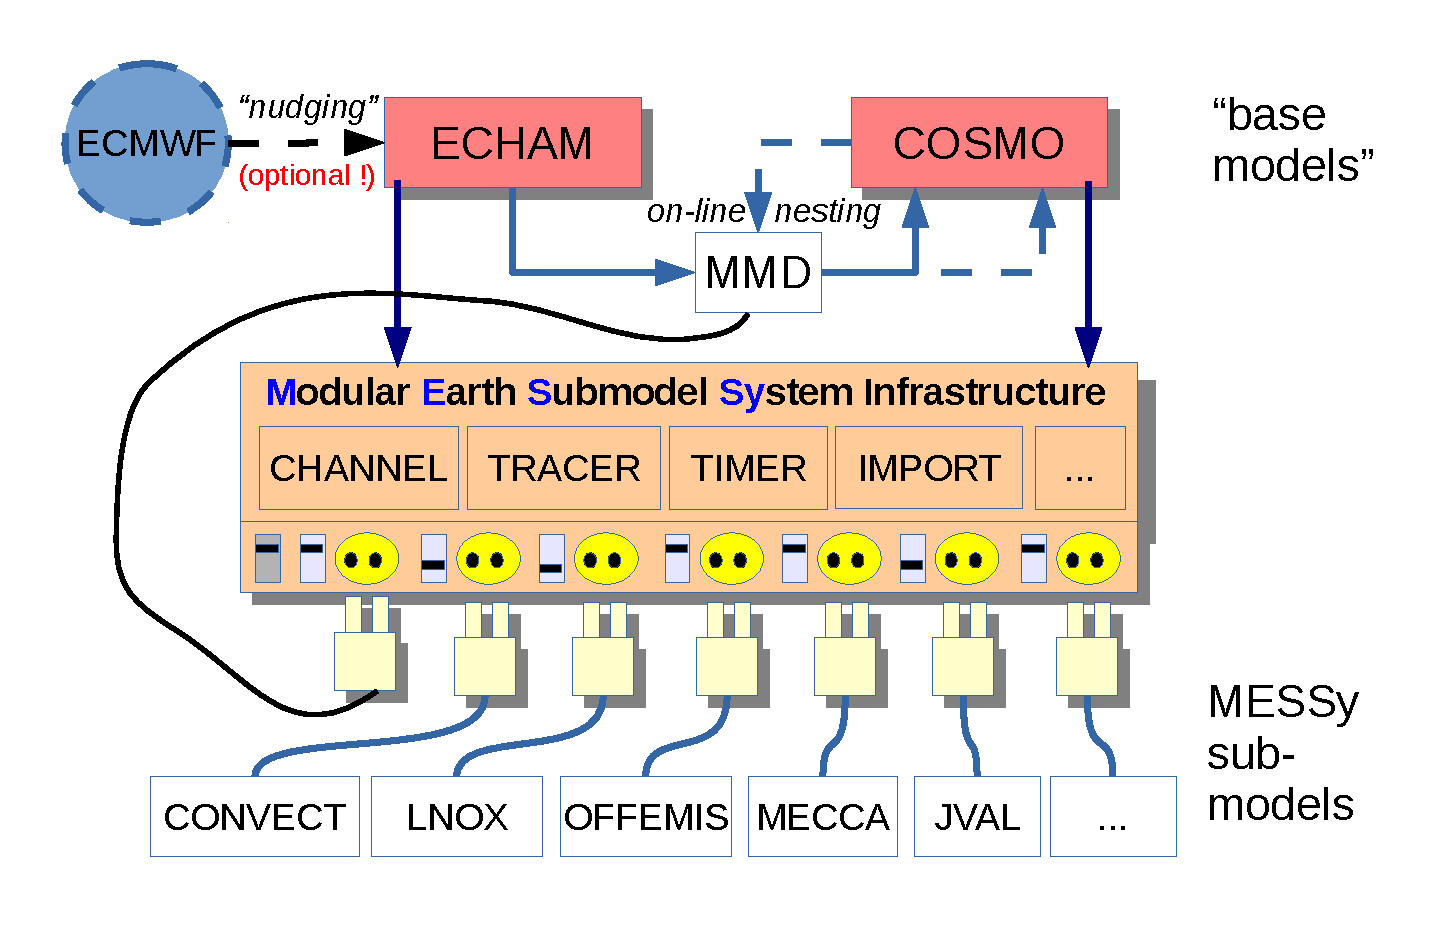
\includegraphics[width=0.9\textwidth]{MECOn_coupling_stecker.pdf} 
\end{center} 
\vspace{-.8cm}
\caption{Illustration of a MECO(n) coupled setup. Each of the
basemodels, ECHAM and COSMO, are coupled internally to MESSy. Externally, 
different instances of these model are nested into each other via MMD.} 
\label{fig:MECOnflux} 
\end{figure*} 
%%%%%%%%%%%%%%%%

\clearpage


%+++++++++++++++++++++++++++++++++++++++++++++++++++++++++++++++++++++++++++
%+++++++++++++++++++++++++++++++++++++++++++++++++++++++++++++++++++++++++++
%+++++++++++++++++++++++++++++++++++++++++++++++++++++++++++++++++++++++++++
\section{The run-scrip \tt xmessy\_mmd}\label{sec:runscript}
The run-script consists of three major sections:
\begin{enumerate}
\item The first section contains batch job scheduler (queueing system)
settings. All schedulers 
MESSy was, so far, used with, are listed in this run-script. New 
queueing systems can be added easily. The user has to activate the appropriate
setup for the computing system he/she is using.
\item The second section is the one which needs specifications according to the 
intended model simulation. Thus this section is subject to changes by every user
for a specific simulation.
\item The last section contains all MESSy and machine specific settings.
These should normally not be changed by a model user. Only, if a new
 system is added, 
 changes are also required in this part of the run-script.
\end{enumerate}

Here, we focus on the second block of the run-script,
i.e., that part that needs to be adapted by the user for a specific model setup.
Its start is indicated in the run-script by the comment:
\begin{verbatim}
#############################################################################
### USER DEFINED GLOBAL SETTINGS
#############################################################################
\end{verbatim}
The settings are described one after the other  as they are
aligned in the script: 
\begin{itemize}
\item \verb|EXP_NAME|: This is the name of the experiment. This variable is
copied to the CHANNEL\footnote{The CHANNEL submodel is described in detail in the
electronic supplement of \cite{Joeckel10a}.}  namelist. All CHANNEL output files 
will start with this
experiment name. Its maximal length is 14 characters.
\item \verb|WORKDIR|: This is the directory in which the simulation is actually
performed. In this directory subdirectories are created by the run-script and all
 data written during the simulation are placed into these (sub-)directories.
For each model instance (see below) a subdirectory named by the instance number
is created.
 Note: for most scheduling systems the log-file will be placed in the directory 
from which the run-script is submitted.
\item \verb|START_YEAR|, \verb|START_MONTH|, \verb|START_DAY|, \verb|START_HOUR|, \verb|START_MINUTE|, \verb|START_SECOND|:
These are the start date/time components. They are copied to the 
TIMER\footnote{The TIMER submodel is described in detail in the
electronic supplement of \cite{Joeckel10a}.} namelist 
defining the start date/time of the simulation. Additionally, they are copied to
 all namelists which require start time dependent entries. For instance, for an 
emission file 
containing monthly averaged emission fluxes the knowledge of the month in which
the simulation starts is required. Nudging is another important example 
depending on the start date components.
\item \verb|STOP_YEAR|, \verb|STOP_MONTH|, \verb|STOP_DAY|, \verb|STOP_HOUR|, \verb|STOP_MINUTE|, \verb|STOP_SECOND|:
These date components are copied to the TIMER and nudging namelists to
determine the end of a simulation.
\item \verb|RESTART_INTERVAL=1|, \verb|RESTART_UNIT=months|: These entries
determine the frequency with which restart files are written. 
\verb|RESTART_UNIT| provides the unit of the
interval, while \verb|RESTART_INTERVAL| defines the number of steps in
unit \verb|RESTART_UNIT|. These parameters are copied to the TIMER namelist. 
|
\item \verb|NML_SETUP|: This variable determines which namelist setup is used.
In the subdirectory \verb|messy/nml/| within the MESSy distribution different
namelist setups are available. 
\verb|NML_SETUP| selects the name of the subdirectory,
which should be used. If an ECHAM5/MESSy-only simulation is 
performed, the subdirectory contains only the namelists required for an 
ECHAM5/MESSy simulation. For a COSMO/MESSy only simulation, the
namelist subdirectory contains only the namelists required for one
COSMO/MESSy model instance.
For the coupled simulations the respective directory contains as 
many subdirectories as coupled instances exist. 
The numbers in the coupling layout 
(see below) are the same as the numbers of the namelist
subdirectories. The namelists for the coupled setups are all placed in
a subdirectory called \verb|MMD|.

\item \verb|OFT| (Output File Type): At the time being it can be chosen between
 netCDF\footnote{\it http://www.unidata.ucar.edu/software/netcdf/} and 
parallel-netCDF\footnote{\it http://www.mcs.anl.gov/parallel-netcdf},
 if the latter is available. This flag is copied to 
the CHANNEL namelist.
\item \verb|QWCH|: This should be set to the available wall-clock
hours defined by the schedule and is copied to the QTIMER\footnote{The
QTIMER submodel is described in  
\cite{Joeckel10a}.}  namelist.
\item \verb|INSTANCE|: This gives the number and type of model instances
running simultaneously in the MPI environment. The names ``ECHAM5''
and ``COSMO'' indicate whether in this instance an ECHAM5/MESSy model
or a COSMO/MESSy  model is executed.
\begin{verbatim}
### =========================================================================
### SELECT MODEL INSTANCES: 
###  - ECHAM5, MPIOM, CESM1 (always first, if used)
###  - COSMO
###  - other = MBM
### =========================================================================
INSTANCE[1]=ECHAM5
INSTANCE[2]=COSMO
INSTANCE[3]=COSMO
\end{verbatim}
If ECHAM5/MESSy is the coarsest parent model ({\it master parent} or
{\it patriarch}), this needs
to be the {\bf first} instance.
If ECHAM5/MESSy or COSMO/MESSy are run alone, only one instance is set.
The run-script can also be used to run other MESSy models, e.g., the
generic MESSy basemodel BLANK (\verb|INSTANCE[1]=blank|), CAABA
(\verb|INSTANCE[1]=caaba|, \cite{Sander2011}),
 MPIOM (\verb|INSTANCE[1]=mpiom|, \cite{Pozzer11b}) or CESM1 (\verb|INSTANCE[1]=CESM1|, \cite{Baumgaertner2016}) can be
 run as autonomous model with the same run-script.
\item \verb|MMDPARENTID|: For each model instance  the server of the model needs 
to be determined. The server of a model is defined by its instance number.
\begin{verbatim}
### =========================================================================
### SET MMD PARENT IDs (-1: PATRIARCH)
### =========================================================================
MMDPARENTID[1]=-1
MMDPARENTID[2]=1
MMDPARENTID[3]=2
\end{verbatim}
The {\it patriarch} is indicated by ``-1'' because 
the {\it patriarch} has no server itself. 
For the above example, the server of instance number 2
 is the first instance, i.e., the ECHAM5/MESSy model. The second
 instance itself is server to the third
 instance. \verb|MMDPARENTID[3]=1| would mean that the 
third model also gets its data directly from ECHAM5/MESSy.
\item \verb|NPX|, \verb|NPY| and \verb|NVL|: \verb|NPX| and \verb|NPY| 
determine the parallel domain decomposition
of the model instances in x and y direction, respectively. For the
COSMO model these  
are copied to \verb|nprocx| and \verb|nprocy| in the COSMO namelist 
\verb|&RUNCTL| in the \verb|INPUT_ORG.nml| namelist file. 
For ECHAM5/MESSy
 these entries are copied to \verb|NPROCA| and \verb|NPROCB| in the
\verb|&RUNCTL| namelist of the \verb|ECHAM5.nml| namelist file.
So far, \verb|NVL| was only of importance for ECHAM5/MESSy, as the
vector length \verb|NPROMA| is set to \verb|NVL|. For the COSMO model
versions containing the unified COSMO-ICON model physics \verb|NVL|
also defines the block length used in the COSMO physics.
\item ECHAM5 specific settings:
\begin{itemize}
\item \verb|ECHAM5_HRES|,\verb|ECHAM5_VRES|: Spectral and vertical resolution
of ECHAM5. \verb|ECHAM5_HRES| is for example one of 
\verb|(T106, T85, T63, T42, T31, T21, T10)|, whereas \verb|ECHAM5_VRES|
is for example, one 
of \verb|(L19, L31ECMWF, L41DLR, L39MA, L90MA)|.
Note that ECHAM5 always requires initial data in the chosen resolution.
\item \verb|MPIOM_HRES|, \verb|MPIOM_VRES|: horizontal and vertical 
resolution of MPIOM, when it is chosen as a
submodel. \verb|MPIOM_HRES| is for example one out of 
\verb|(GR60, GR30, GR15, TP04, TP40)| and \verb|MPIOM_VRES| one out of 
\verb|(L3, L20, L40)|.

\item \verb|ECHAM5_NUDGING|: This {\footnotesize LOGICAL } is set to T, 
if nudging of the ECHAM5 model 
is requested. The nudging coefficients in the ECHAM5 namelist file (namelist
\verb|&NDGCTL|) must be set accordingly. 
\item \verb|ECHAM5_LAMIP|: Switch for using sea-surface temperature (sst) and  
sea-ice forcing via AMIP-like data for ECHAM5.
\item \verb|NML_ECHAM|: name of the ECHAM5 namelist file. As the ECHAM5
namelists include some resolution dependent entries, it is convenient to work
 with resolution dependent ECHAM5 namelist files.
\end{itemize}
\item user-defined specific namelist files, e.g., depending on the
 resolution, the start date, etc.
\item COSMO specific settings: \verb|COSMO_SUBDIR|, \verb|COSMO_EXTNAME| and \verb|COSMO_EXTGRID|:
These entries are used to determine the INT2COSMO namelist entries required to
 access the external data file.  
\verb|COSMO_EXTNAME| fills the namelist entry \verb|ylmext_lfn|
 and \verb|COSMO_EXTGRID| contains the horizontal grid sizes of the
external data file, which naturally depend on the external data file and are
required as individual entries in the INT2COSMO namelist \verb|&DATA|.
 \verb|ylmext_cat| is filled by \verb|COSMO_EXTDIR|, which is composed of a 
 general data input path (\verb|INPUTDIR_COSMO_EXT|) and a subdirectory 
(\verb|COSMO_SUBDIR|) in this input path. 
\verb|COSMO_SUBDIR| has to be defined individually for each instance, while
 a default value (as part of the standard MESSy input directory) 
exists for \verb|INPUTDIR_COSMO_EXT|. However, \verb|INPUTDIR_COSMO_EXT| 
can also be user-defined for each individual instance.
\begin{verbatim}
### -> COSMO_EXTDIR[.] = ${INPUTDIR_COSMO_EXT[.]}/$COSMO_SUBDIR[.]
COSMO_SUBDIR[1]=
COSMO_EXTNAME[1]=
COSMO_EXTGRID[1]=

COSMO_SUBDIR[2]=climatology
COSMO_EXTNAME[2]=europe.nc
COSMO_EXTGRID[2]="ie_ext=101, je_ext=107,"

COSMO_SUBDIR[3]=external
COSMO_EXTNAME[3]=lm_d1_g0.165_463x383
COSMO_EXTGRID[3]="ie_ext=463, je_ext=383,"
\end{verbatim}
The number in brackets is the instance number. In the example with ECHAM5/MESSy
 as first instance, the block with instance number 1 must be empty.
\end{itemize}
The above listed variables need to be set.
Here, additional variables are listed, which can be set, if the default 
settings should not be used:
\begin{itemize}
\item \verb|BASEDIR|: This is the directory of the model distribution.
\item \verb|DATABASEDIR|: Base directory for model initial data.
\item \verb|INPUTDIR_ECHAM5_INI|: Directory containing the input data for the
ECHAM5 model.
\item \verb|INPUTDIR_ECHAM5_SPEC|: Directory containing the \verb|*_spec| and 
\verb|*_surf| files for the ECHAM5 initialisation.
 These depend on the resolution and start date. 
With \verb|INPUTDIR_ECHAM5_SPEC|, the user can put the initial files specific 
for the start date of his/her simulation into a private directory and use the 
default directory for the others.
\item \verb|INPUTDIR_NUDGE|: Directory of the nudging data files for ECHAM5.
\item \verb|FNAME_NUDGE|: Name template of the ECHAM5 nudging data files. 
This differs depending on the source of the data. (ERA40/ERA-Interim or analysis (ANALY)).
\item \verb|INPUTDIR_AMIP|: Directory of the sst and sea-ice data for ECHAM5.
\item \verb|INPUTDIR_MPIOM|: Directory containing MPIOM input data.
\item \verb|INPUTDIR_COSMO_EXT|: Directory containing COSMO input
(``external'') data.
\item \verb|INPUTDIR_COSMO_BND|: Directory containing COSMO initial and
boundary data, if COSMO is run in stand-alone mode or as {\it patriarch}.
\item \verb|INPUTDIR_CESM1|: Directory containing CESM1 input data.
\item \verb|INPUTDIR_MESSY|: Directory containing input data for the MESSy
 submodels.
\item \verb|USE_PREREGRID_MESSY|: It is possible to provide the MESSy input data
 on the specific horizontal Gaussian grid, i.e., in pre-regridded form. This is
used when \verb|USE_PREREGRID_MESSY = T|. Note: this only works for ECHAM5/MESSy.
\item SPECIAL MODES:
\begin{itemize}
\item \verb|SERIALMODE|: switch on, if basemodel was compiled without
MPI\footnote{message passing interface} parallelisation.
\item \verb|TESTMODE|: Test mode of the run-script, exits before starting the
executable.
\item \verb|MEASUREMODE|: Measure memory use. This is only available on 
specific machines. 
\item \verb|PROFMODE|: A special mode, for performance 
monitoring, which is only available on specific machines: Possible
settings are \verb|TPROF|, \verb|VAMPIR| or \verb|SCALASCA|. Additionally, the
parameter \verb|PROFCMD| is required.
\end{itemize}
\end{itemize}
The user specified block ends with the marker:
\begin{verbatim}
#############################################################################
#############################################################################
### =========================================================================
#############################################################################
### DO NOT CHANGE ANYTHING BELOW THIS LINE !!!
#############################################################################
### =========================================================================
#############################################################################
#############################################################################
\end{verbatim}

%+++++++++++++++++++++++++++++++++++++++++++++++++++++++++++++++++
%+++++++++++++++++++++++++++++++++++++++++++++++++++++++++++++++++
%+++++++++++++++++++++++++++++++++++++++++++++++++++++++++++++++++
\section{The MMD2WAY namelists}\label{sec:namelist}
The namelist file of the submodel MMD2WAY consists of five different
namelists:
\begin{itemize}
\item \verb|&CTRL|: the overall control namelist read by the child model
\item \verb|&CPL_PARENT|: a namelist generally driving the coupling from the
parent model side (read by the parent model).
\item \verb|&CPL_PAR_CHILD|: an arbitrary number of these namelists,
specifying the transfer of child fields to the parent model individually for
each coupled instance (read by the parent model).
\item \verb|&CPL_CHILD|: a namelist generally driving the coupling from the
child model side (read by the child model).
\item \verb|&CPL_CHILD_ECHAM| or \verb|&CPL_CHILD_COSMO|: namelist specifying
which fields are required from the parent model for the child model (read by
the child model). For simplicity reasons two different namelists are provided
for the two possible parent models ECHAM5 or COSMO.
\end{itemize}

In the following the individual namelists are described.
First the namelists read by the child models are explained.

\subsection{\protect\&CTRL}\label{sec:nmlctrl}
%+++++++++++++++++++++++++++++++++++++++++++++++++++++++++++++++++
%+++++++++++++++++++++++++++++++++++++++++++++++++++++++++++++++++
\begin{figure*}
\footnotesize
{\blockcode 
\begin{verbatim} 
! -*- f90 -*-
&CTRL
! WRITE ORIGINAL INT2COSMO  OUTPUT
l_I2Cori_output = .FALSE.
! do not use steps
WRITEI2C_IOEVENT  = 1,'hours','exact',0 
! INITIALSE VARIABLES
!l_forcevars = .TRUE.,
!forcevars = "T_SO;W_SO;T_S;W_I;QV_S;W_SNOW;T_SNOW",
!forcefile = "/DATA/COSMO/soil_ini/lffd2001010100.nc"
/
\end{verbatim} 
}
\vspace*{-.7cm}
\caption{Example {\tt \&CTRL}-namelist of the MMD2WAY namelist file ({\tt mmd2way.nml})} 
\label{fig:nmlctrl} 
\end{figure*} 
The \verb|&CTRL|-namelist (Fig.\ \ref{fig:nmlctrl}) consists of two
blocks of namelist variables: one to trigger original INT2LM output
and the other for an improved initialisation of the soil variables:
\begin{itemize}
\item two variables are required to trigger the original output: one
{\footnotesize LOGICAL }switch and one {\it event}\footnote{The generic submodel TIMER and the definition and  
functionality of {\it events} are described in the manual about TIMER within the
 electronic supplement of \cite{Joeckel10a}.}:
\begin{itemize}
\item If the {\footnotesize LOGICAL} \verb|l_I2Cori_output| is
set \verb|.TRUE.| (default: \verb|.FALSE.|), INT2COSMO produces its original output, i.e., the
initial and boundary files are written during the on-line coupled
simulation. They can be used later on to perform off-line COSMO
simulations.
Note: this only works for original INT2LM output, implying that MESSy
specific boundary data (e.g., for chemical species) are not written to these files.

\item The {\it event} (\verb|WRITEI2C_IOEVENT|) determines the
temporal interval in which files are written, if 
\verb|l_I2Cori_output = .TRUE.|.
\end{itemize}

\item the forcing of specific variables requires three namelist variables:
\begin{itemize}
\item the {\footnotesize LOGICAL} \verb|l_forcevars| to switch on
this specific feature (default: \verb|.FALSE.|).
\item the string variable \verb|forcevars| containing the names of all
variables to be re-initialised by this procedure.
\item the string variable \verb|forcefile| providing the path and the name
of the file containing the data.
\end{itemize}
Note: the COSMO domain definition in \verb|forcefile| has to
be exactly the same as in the simulation performed.
\end{itemize}

%+++++++++++++++++++++++++++++++++++++++++++++++++++++++++++++++++
\subsection{\protect\&CPL\_CHILD}\label{sec:nmlcplchild}
The \verb|&CPL_CHILD|-namelist (Fig.\ \ref{fig:nmlcplchild}) is read by
MMD2WAY\_CHILD and determines the interval of coupling between this specific
child and its parent model. The namelist contains two 
{\it events}:
\begin{itemize}
\item the first (\verb|CPL_IOEVENT|) determines the interval of the
coupling to the parent model, i.e., how often data are exchanged
between parent and child model, 
\item the second {\it event} (\verb|READEXT_IOEVENT|) determines the
update interval of the
 external data required by \verb|INT2COSMO|.
\end{itemize}

For the definition of the coupling {\it event} the user has
to be aware of two limitations:
\begin{itemize}
\item To simplify the data exchange between the
coupled models, the coupling interval is internally converted to seconds. As 
this conversion is not well defined for the units \verb|'months'| and
\verb|'years'|, the coupling interval must be specified in \verb|'steps'|, 
\verb|'seconds'|, \verb|'minutes'|, \verb|'hours'| or \verb|'days'|.
\item As for all other {\it events}, the user has to define a multiple of the 
model time step length, otherwise the simulation is terminated. Especially,
 the coupling interval is a multiple of the time steps of the
 child \underline{and} the parent model.  
\end{itemize}

\begin{figure*}
\footnotesize
{\blockcode
\begin{verbatim} 
&CPL_CHILD
CPL_IOEVENT      = 10,'minutes','first',0
READEXT_IOEVENT  = 1,'years','none',0
/
\end{verbatim} 
}
\vspace*{-.7cm}
\caption{Example {\tt \&CPL\_CHILD}-namelist of the MMD2WAY namelist file ({\tt mmd2way.nml}).} 
\label{fig:nmlcplchild} 
\end{figure*} 

%+++++++++++++++++++++++++++++++++++++++++++++++++++++++++++++++++
\subsection{\protect\&CPL\_CHILD\_ECHAM and \&CPL\_CHILD\_COSMO}\label{sec:nmlcplchildEorC}
The second part of the namelist file, which is child model relevant, contains a list of {\it exchange fields} 
required to fully initialise and drive the respective child COSMO/MESSy model. 
The {\it exchange fields} are unambiguously identified by their 
{\it channel} and {\it channel object} names.
 As these usually differ between ECHAM5/MESSy and COSMO/MESSy, 
the namelists depend on the parent model.
\begin{figure*}
\footnotesize
{\blockcode
\begin{verbatim} 
&CPL_CHILD_ECHAM
! ###############################################################################
!
! ###############################################################################
! ### MANDATORY FIELDS
! ###############################################################################
!********************************************************************************
FIELD(1)   = 'g3b','aps', 'COSMO_ORI', 'PS', '', F, F, F , ''     
!********************************************************************************
FIELD(2)   = 'ec2cosmo','T_S', 'COSMO_ORI','T_S', '', T, T, F, ''
!********************************************************************************
FIELD(3)   = 'g3b','slf', 'COSMO_ORI','FR_LAND', '', T, F, F, '' 
!********************************************************************************
FIELD(4)   = 'g1a','tm1', 'COSMO_ORI','T', '', T, T, F, ''      
!********************************************************************************
FIELD(5)   = 'g1a','qm1', 'COSMO_ORI','QV', '', T, T, F, ''     
!********************************************************************************
FIELD(6)   = 'g1a','xlm1', 'COSMO_ORI','QC', '', T, T, F, ''    
!********************************************************************************
FIELD(7)   = 'g1a','xim1', 'COSMO_ORI','QI', '', T, T, F, ''    
!********************************************************************************
FIELD(8)   = 'g2a','um1', 'COSMO_ORI','U', '', T, T, F, ''      
!********************************************************************************
FIELD(9)   = 'g2a','vm1', 'COSMO_ORI','V', '', T, T, F, ''     
!********************************************************************************
FIELD(10)  = 'g3b','geosp', '#XXX','FIS', '', F, F, F, ''       
!********************************************************************************
FIELD(11)  = 'g3b','wl', 'COSMO_ORI','W_I', '', T, F, F, ''    
!********************************************************************************
FIELD(12)  = 'g3b','sni', 'COSMO_ORI','W_SNOW', '', T, T, F, '' 
!********************************************************************************
FIELD(13)  = 'g3b','tsi', 'COSMO_ORI','T_SNOW', '', T, T, F, ''  
!********************************************************************************
FIELD(14)  = 'ec2cosmo','W_SO_REL', 'COSMO_ORI','W_SO', '', T, F, F, ''
! ###############################################################################
! ### OPTIONAL FIELDS
! ###############################################################################
FIELD(20)  = 'Test','Test_Ar', 'mmd2way_child','Test_Ar', '', F, F, F, '' 
!********************************************************************************
FIELD(21)  = 'tracer_gp_m1','O3', 'tracer_gp','O3', 'QFTV', T, T, F, ''
!********************************************************************************
FIELD(22)  = 'ptrac_gp','wetradius', 'ptrac_gp','wetradius', 'QTFV', T, F, F, ''
!********************************************************************************
FIELD(23)  = 'jval_gp','J_O1D', 'mmd2way_child','J_O1D', 'QFTV', F, F, T, 'GP_3D_MID'
!********************************************************************************
FIELD(24)  = 'import_grid','RGT0012_CO','mmd2way_child','RGT0012_CO','M',F,F,T,'#UNKNOWN'
! ###############################################################################
/
\end{verbatim} 
}
\vspace*{-0.7cm}
\caption{Example {\tt \&CPL\_CHILD\_ECHAM} namelist of MMD2WAY namelist file ({\tt mmd2way.nml}).} 
\label{fig:nmlcplchildecham} 
\end{figure*} 

%+++++++++++++++++++++++++++++++++++++++++++++++++++++++++++++++++
%\subsection{\protect\&CPL\_CHILD\_COSMO}
\begin{figure*}
\footnotesize
{\blockcode
\begin{verbatim} 
&CPL_CHILD_COSMO
! ###############################################################################
!
! ###############################################################################
! ### MANDATORY FIELDS
! ###############################################################################
FIELD(1)  = 'COSMO','ps', 'COSMO_ORI','PS', '', F, F, F, ''
!********************************************************************************
FIELD(2)  = 'COSMO','t_s', 'COSMO_ORI','T_S', '', T, T, F, ''
!********************************************************************************
FIELD(3)  = 'COSMO_ORI','FR_LAND', 'COSMO_ORI','FR_LAND', '', T, F, F, ''
!********************************************************************************
FIELD(4)  = 'COSMO','tm1','COSMO_ORI','T', '', T, T, F, ''
!********************************************************************************
FIELD(5)  = 'COSMO','qv','COSMO_ORI','QV', '', T, T, F, ''
!********************************************************************************
FIELD(6)  = 'COSMO','qc','COSMO_ORI','QC',  '', T, T, F, ''
!********************************************************************************
FIELD(7)  = 'COSMO','qi','COSMO_ORI','QI',  '', T, T, F, ''
!********************************************************************************
FIELD(8)  = 'COSMO','um1','COSMO_ORI','U',  '', T, T, F, ''
!********************************************************************************
FIELD(9)  =  'COSMO','vm1', 'COSMO_ORI','V','', T, T, F, ''
!********************************************************************************
FIELD(10) = 'COSMO','t_so', 'COSMO_ORI','T_SO', '', T, F, F, ''
!********************************************************************************
FIELD(11) = 'COSMO','w_so','COSMO_ORI','W_SO',  '', T, F, F, ''
!********************************************************************************
FIELD(12) = 'COSMO','t_snow', 'COSMO_ORI','T_SNOW', '', T, T, F, ''
!********************************************************************************
FIELD(13) = 'COSMO','w_snow', 'COSMO_ORI','W_SNOW', '', T, T, F, ''
!********************************************************************************
FIELD(14) = 'COSMO','w_i', 'COSMO_ORI','W_I', '', T, F, F, ''
!********************************************************************************
FIELD(15) = 'COSMO','qv_s', 'COSMO_ORI','QV_S', '', T, T, F, ''
!********************************************************************************
FIELD(16) = 'COSMO_ORI','FRESHSNW', 'COSMO_ORI','FRESHSNW', '', T, F, F, ''
!********************************************************************************
FIELD(17) = 'COSMO_ORI','HSURF', 'COSMO_ORI','HSURF', '', T, F, F, ''
!********************************************************************************
FIELD(18) = 'COSMO','ppm1', 'COSMO_ORI','PP', '', T, T, F, ''
!********************************************************************************
FIELD(19) = 'COSMO_ORI','SOILTYP', 'COSMO_ORI','SOILTYP', '', T, F, F, ''
!***************************************************************************
! ###############################################################################
! ### OPTIONAL FIELDS
! ###############################################################################
FIELD(20) = 'Test','Test_Ar', 'mmd2way_child','Test_Ar', '', F, F, F, ''
!********************************************************************************
!********************************************************************************
FIELD(21) = 'tracer_gp_m1','all', 'tracer_gp','*', 'QFTV', T, T, F, ''
!********************************************************************************
! ###############################################################################
/
\end{verbatim} 
}
\vspace*{-0.7cm}
\caption{Example {\tt \&CPL\_CHILD\_COSMO}-namelist of MMD2WAY namelist file ({\tt mmd2way.nml}). } 
\label{fig:nmlcplchildcosmo} 
\end{figure*} 
Figure \ref{fig:nmlcplchildecham} shows a typical \verb|&CPL_CHILD_ECHAM|
namelist for the 
coupling to ECHAM5/MESSy and Fig.\ \ref{fig:nmlcplchildcosmo} shows the
namelist   
\verb|&CPL_CHILD_COSMO| used for the coupling to a COSMO/MESSy model as parent. 
The structure of the two namelists is identical. 
Each {\it exchange field}
 is defined by one namelist entry of {\footnotesize TYPE}
 \verb|FIELD|:
\begin{verbatim}
FIELD(.) = 'PARENT_CHANNEL', 'PARENT_OBJECT', 'CHILD_CHANNEL', 'CHILD_OBJECT' 
         , 'INTERPOL_METHOD', L_INITIAL, L_BOUND, L_INPUT, 'CHILD_REPR'
\end{verbatim}
\verb|FIELD| is a variable of {\footnotesize TYPE} \verb|T_C_EXCH_IO|:
\begin{verbatim}
  TYPE CHAOBJ_NAMES
     CHARACTER(LEN=STRLEN_CHANNEL)  :: CHA = '' ! CHANNEL NAME 
     CHARACTER(LEN=STRLEN_OBJECT)   :: OBJ = '' ! OBJECT  NAME 
  END TYPE CHAOBJ_NAMES

  TYPE T_C_EXCH_IO
     TYPE(CHAOBJ_NAMES) :: PARENT
     TYPE(CHAOBJ_NAMES) :: CHILD
     CHARACTER(LEN=4)   :: C_INTERPOL = ''      ! INTERPOLATION METHOD
     ! Specify target field
     LOGICAL            :: L_INITIAL  = .FALSE. ! INITIAL FIELD
     LOGICAL            :: L_BOUND    = .FALSE. ! BOUNDARY FIELD
     LOGICAL            :: L_INPUT    = .FALSE. ! INPUT FIELD 
     CHARACTER(LEN=STRLEN_MEDIUM) :: C_REPR ='' ! REPRESENTATION STRING
  END TYPE T_C_EXCH_IO

  ! MAXIMAL NUMBER OF EXCHANGE FIELDS
  INTEGER, PARAMETER                            :: NMAX_EXCH = 1000
  TYPE(T_C_EXCH_IO), DIMENSION(NMAX_EXCH), SAVE :: FIELD
\end{verbatim}

\begin{itemize}
\item The first two structure components of {\footnotesize TYPE CHARACTER}
specify the {\it channel} and {\it channel object} name of the 
{\it exchange field} on the parent side. For instance, the surface pressure
field in ECHAM5/MESSy
 is defined in the  {\it channel} 'g3b' with the {\it channel
object} name 'aps' (see \verb|FIELD(1)| in Fig.\ \ref{fig:nmlcplchildecham}).
\item  The third and fourth structure components of 
{\footnotesize TYPE CHARACTER} name the {\it channel} and {\it channel object}
 of the {\it exchange field} in the client model. For \verb|FIELD(1)| in 
Fig.\ \ref{fig:nmlcplchildecham} this is the {\it channel} 'COSMO\_ORI' and the
{\it channel object} 'PS'.

For the child {\it channel object} names wildcards are allowed.
A \verb|'*'| replaces an arbitrary number of characters or digits, whereas
\verb|'?'| replaces exactly one character or digit. Based on wildcards, it 
is possible to address a number of {\it channel objects} of one {\it channel}
 with one namelist entry. The only restriction for wildcard usage is that the 
 name of the {\it channel object} on the parent side must be identical to that 
 on the child side\footnote{This is usually not the case for the basemodels
 ECHAM5 and COSMO, but for the MESSy submodels.},
 because the names for the parent {\it channel object}s are
 overwritten by the child {\it channel object} names, if wildcards are used.
 For instance, an entire tracer set can be coupled by setting 
\verb|'CHILD_CHANNEL', 'CHILD_OBJECT'| to \verb|'tracer_gp', '*'| or all 
photolysis rates are coupled by  \verb|'jval_gp', 'J_*'|.
Due to the initialisation of prognostic variables at the beginning of 
each time step 
in COSMO/MESSy in the subroutine \verb|initialize_loop| in \verb|lmorg.f90|
the parent {\it channel} for the coupling of the tracers needs to be 
\verb|'tracer_gp'|. In case of ECHAM5 the fields in \verb|'tracer_gp'|
and  
\verb|'tracer_gp_m1'| are identical at the beginning of the time loop.

\item The fifth structure component is a {\footnotesize CHARACTER} of length 4.
 It determines the interpolation method. This is only required for the 
{\it additional fields}, as for the {\it INT2COSMO inherent fields} the 
interpolation method is determined inside of INT2COSMO. Possible interpolation
methods are: 'Q'  for quadratic;  'L' for linear and 'M' for match point
interpolation. Additionally 'C' for conservative remapping via the MESSy
submodel GRID has been added to INT2COSMO.
Thus the first character must be set to one of 'Q', 'L', 'M' or 'C'.  The
second and the third character demand monotonicity and positive definiteness, respectively,
 if set to ’T’. The default value, however, is ’F’. If the fourth character is 
 'V' or 'W', the field will additionally be interpolated in the vertical
 direction via 
 the INT2COSMO inherent spline method ('V') or via NREGRID ('W'). However, 
 this is only possible for 3D- or 4D-fields of which the number of vertical 
 levels equals the number of vertical levels in the model. For instance, the 
 fifth string of FIELD(21) in \verb|&CPL_CHILD_ECHAM| determines that the ozone 
 tracer is interpolated horizontally by quadratic interpolation and in addition
  vertically using the spline method. No care is taken to ensure monotonicity,
  but positive  definiteness is requested. 
\item The next three logicals in the FIELD(:) entry indicate the data
destination  ({\it initial},  
{\it boundary} or {\it input}) of the interpolated field.
{\it Mandatory fields} can be {\it initial} and {\it boundary fields}.
 For the {\it mandatory fields} the entries for the data destination types in 
the namelist could be omitted, as they are set according to the COSMO variables 
\verb|yvarini| and \verb|yvarbd|. These variables list the {\it initial} and 
{\it boundary fields} required for the chosen COSMO setup. 
If {\it initial} or {\it boundary fields} are required according to 
\verb|yvarini| or \verb|yvarbd| and the data destination flags are not set 
\verb|.TRUE.| in the namelist, the namelist settings are ignored.
If a field destination is requested (in addition to \verb|yvarini| or 
\verb|yvarbd|) as {\it initial} or {\it boundary field}, however, this request
 is not overwritten. In other words, if the field is requested
 in the namelist or the COSMO model, it will be processed.
 
 For the {\it optional fields} the choice of {\it initial} and/or {\it boundary}
 and of {\it input} destination is exclusive, as {\it input} already 
implies {\it initial} and the provision of {\it boundary} data  is meaningless, 
since the field is overwritten each coupling time step.
For instance, for the prognostic variables water vapour and cloud water 
(\verb|FIELD(5)| and \verb|FIELD(6)| in Fig.\ \ref{fig:nmlcplchildecham}) the 
 calculation of the {\it initial} and  {\it boundary fields} is requested,
 whereas for the land fraction (\verb|FIELD(3)| in  Fig.\ \ref{fig:nmlcplchildcosmo})
 only the {\it initial field}  is calculated. As tracers are prognostic 
variables, {\it initial} and {\it boundary fields} are requested for ozone 
(\verb|FIELD(21)|). In contrast, the fields \verb|FIELD(23)| and
 \verb|FIELD(24)| are {\it input fields}.

\item The last component of the variable \verb|FIELD| contains the
 {\it representation}\footnote{For a description of {\it representations} see
 the 
 CHANNEL manual, which is part of the electronic supplement of 
\cite{Joeckel10a}.} of the childs {\it channel object}. It is only 
required for {\it additional fields}, for which \verb|L_INPUT|
is \verb|.TRUE.|.  
In this case the memory for a field is neither defined by a MESSy submodel nor 
by the basemodel itself and consequently, the submodel MMD2WAY\_CHILD has to
define the respective  
{\it channel object} itself, which is indicated by
giving \verb|'mmd2way_child'| as  child {\it channel} name in the
third \verb|FIELD| entry in the \verb|&CPL_CHILD_ECHAM| 
namelist. For these fields the {\it representation} must be known as
MMD2WAY\_CHILD  needs to allocate the memory for the respective field itself.
 
For instance, in \verb|FIELD(23)| in the \verb|&CPL_CHILD_ECHAM| namelist, the 
photolysis rate of $\rm O^1D$ from the ECHAM5/MESSy submodel JVAL ({\it channel}
 name \verb|'jval_gp'|, {\it channel object} name \verb|'J_O1D'|) is defined
 as {\it input field} of the regional model. If JVAL is not switched on in 
COSMO/MESSy, MMD2WAY\_CHILD needs to define the {\it channel object} itself. 
The photolysis rates are defined at the center of the grid boxes.
Thus the {\it representation} of a photolysis rate is a priori known and the 
{\it representation} name for the child model can be specified (here,
\verb|'GP_3D_MID'|).

In cases where the {\it representation} is not a priori known, it is deduced
from the {\it representation} of the parent {\it channel object}. This heuristic
procedure, triggered by the entry \verb|'#UNKNOWN'| (see \verb|FIELD(24)| in
 Fig.\ \ref{fig:nmlcplchildecham}), 
is described in detail in Sect.~\ref{srt:get_CPLDATA}.
\end{itemize}

In addition to the coupling of standard 2D and 3D data fields, the coupling of
4D data fields is implemented. They are treated exactly in the same way.
However, due to differences in the implementation of tracers \citep{Joeckel08a}
and the implementation of prognostic variables in the COSMO 
model, it is not possible to couple the 4D tracer field
 directly. Nevertheless, each 
individual tracer can be coupled, as the individual tracers are accessible
 as 3D {\it channel objects} (e.g.,\ \verb|FIELD(21)| in Fig.\ 
\ref{fig:nmlcplchildecham}). To simplify the handling of large tracer sets,
wildcards  
can be used for the child {\it channel object} names in the namelist: 
\verb|'*'| replaces an arbitrary number of characters, \verb|'?'|
replaces exactly one character. For instance, \verb|FIELD(25)| would request all
tracers available in the {\it channel} \verb|'tracer_gp_m1'|. Of course,
wildcards  
in the {\it channel object} names can be used for other {\it channels} as well.

%+++++++++++++++++++++++++++++++++++++++++++++++++++++++++++++++++
%% \subsection{\protect\&CPL\_PARENT}
%% Currently, the \verb|&CPL_PARENT| namelist is empty, as no parent model
%% specific settings are required.
%% \begin{figure*}[h!]
%% \footnotesize
%% {\blockcode
%% \begin{verbatim} 
%% &CPL_PARENT
%% /
%% \end{verbatim}
%% } 
%% \vspace*{-0.7cm}
%% \caption{Example {\tt \&CPL\_PARENT}-namelist of MMD2WAY namelist file ({\tt mmd2way.nml}). } 
%% \label{fig:nmlcplparent} 
%% \end{figure*} 
%+++++++++++++++++++++++++++++++++++++++++++++++++++++++++++++++++
\subsection{\protect\&CPL\_PAR\_CHILD \label{sec:cplparchild}}
\begin{figure*}[h!]
\footnotesize
{\blockcode
\begin{verbatim} 
&CPL_PAR_CHILD
INSTANCE='002'
lgrh     = .FALSE.,
ldiagonly = .TRUE.,
i_rmy_px = 21,
rdefpc = 30000.,
itype_fw = 2,
PFIELD(1)  = 'g1a','qm1', 'scnbuf','qte', 'tracer_gp','QV', 'GP_3D_MID',1,1,1.
PFIELD(2)  = 'g1a','xlm1','scnbuf','xlte','tracer_gp','QC', 'GP_3D_MID',1,1, 0.5
/
\end{verbatim} 
}
\vspace*{-0.7cm}
\caption{Example {\tt \&CPL\_PAR\_CHILD}-namelist of MMD2WAY namelist file
({\tt mmd2way.nml}). This namelist is specific for the case of ECHAM5/MESSy as parent model.} 
\label{fig:nmlcplparchild1} 
\end{figure*} 
%++++++++++++++
\begin{figure*}[h!]
\footnotesize
{\blockcode
\begin{verbatim} 
&CPL_PAR_CHILD
INSTANCE='003'
RCF = 100,
RCF_IN = 100,
i_rmy_px = 25

PFIELD(1)  = 'tracer_gp','QV', '','', 'tracer_gp','QV', 'GP_3D_MID',1,1, 1.
PFIELD(2)  = 'tracer_gp','QC', '','', 'tracer_gp','QC', 'GP_3D_MID',1,1, 0.5
PFIELD(5)  = 'COSMO_ORI','PS',' ',' ','COSMO_ORI','PS','GP_2D_HORIZONTAL',1,1,1.
/
\end{verbatim} 
}
\vspace*{-0.7cm}
\caption{Example {\tt \&CPL\_PAR\_CHILD}-namelist of MMD2WAY namelist file
({\tt mmd2way.nml}). This namelist is specific for the case of COSMO/MESSy as parent model.} 
\label{fig:nmlcplparchild2} 
\end{figure*} 

Figures \ref{fig:nmlcplparchild1} and \ref{fig:nmlcplparchild2} show two
typical examples for parent coupling 
namelists. Figure \ref{fig:nmlcplparchild1} is specific for
ECHAM5/MESSy as parent model and Fig.\ \ref{fig:nmlcplparchild2} for
COSMO/MESSy as parent model. 

The following parameters can be part of the \verb|&CPL_PAR_CHILD|:
\begin{itemize}
\item \verb|INSTANCE|: a mmd2way.nml namelist file may contain an arbitrary
number of \verb|&CPL_PAR_CHILD| namelists. The {\footnotesize CHARACTER} string
of length 3, '\verb|INSTANCE|', is required to attribute each of these namelist
blocks to one specific coupling instance. The number provided by
the namelist parameter \verb|INSTANCE| refers to the instance number as set in the MMD
coupling namelist file \verb|MMD_layout.nml| written and defined by the run-script \verb|xmessy_mmd|. 
\item \verb|itype_fw|: weight function (see
page \pageref{descript:itype_fw}).
 Default: \verb|itype_fw = 2|
\item \verb|icosexp|: factor as required for \verb|itype_fw = 1|. Default value
is \verb|icosexp = 14|.
\item \verb|damprel|: factor as required for \verb|itype_fw = 2|. Default value
is \verb|damprel = 0.02|.

\item \verb|i_rmy_px|: number of grid boxes which are not coupled back in
addition to the damping zone of the child COSMO model domain. Default
is \verb|i_rmy_px = 0|.

\item \verb|RCF|: scaling factor to avoid grid rounding errors as much as
possible (depends on child model grid resolution). Default value: \verb|RCF = 10000.|
\item \verb|RCF_IN|: scaling factor to avoid grid rounding errors as much as
possible (depends on parent model grid resolution). Default value: \verb|RCF_IN = 10000.|

\item \verb|PFIELD|: definition of the coupling fields. PFIELD has the form
\begin{verbatim}
PFIELD(.)= 'parent_channel','parent_object',
           'parent_tendency_channel','parent_tendency_object',
           'child_channel','child_object', 'representation',
            interpol_method, application_method, nudg_fac
\end{verbatim}
\begin{itemize}
\item \verb|parent_channel|, \verb|parent_object|, \verb|parent_tendency_channel|, \verb|parent_tendency_object|:
specification of the data object which is the target of the exchange process:
\begin{itemize}
\item If the tendency of a prognostic variable should be
changed, \verb|parent_tendency_channel| and \verb|parent_tendency_object|
contain the specification of the tendency object and \verb|parent_channel|
and \verb|parent_object| the specification of the data field of the previous
('-1') time step.
\item If the field itself is changed directly,  \verb|parent_channel|
and \verb|parent_object| contain the specification of the field to change
and \verb|parent_tendency_channel| and \verb|parent_tendency_object| are empty
strings.
In the special case, that the submodel  MMD2WAY\_PARENT needs to allocate the
memory for the 
field itself, \verb|parent_channel| equals \verb|'mmd2way_parent'|.
\end{itemize}
\item \verb|child_channel|, \verb|child_object|: specification of the field in
the child model coupled back to the parent model.
\item \verb|representation|: {\it representation} of the parent object, if it
is created in MMD2WAY\_PARENT itself.
\item \verb|interpol_method|: defines the interpolation method. Currently,
only conservative remapping (\verb|interpol_method = 1|) is implemented.
\item \verb|application_method|: determining the application method.
 Currently, only \verb|application_method = 0| for {\it input fields},
 which should not be weighted in any way and grid point space
 (\verb|application_method = 1|) are defined (see page \pageref{descript:appl}). 
\item \verb|nudg_fac|: nudging factor determining the strength of the forcing
of this specific parent field
\end{itemize}
\item \verb|lgrh| (experimental): use generalised humidity for back
remapping to mirror procedure of INT2COSMO. Default value \verb|lgrh = .FALSE.|.
\item \verb|lfreeslip| (experimental): allows for free (non-nudged) layers at
the surface. Default value \verb|lfreeslip = .FALSE.|.
\item \verb|rdefpc| (experimental): control level (in Pa) for vertical
integration, should be the same as defined for INT2COSMO. Default value 
\verb|rdefpc = 30000. Pa|, i.e., identical to the COSMO namelist default value. 
\item \verb|lcpl_gs| (experimental): child to parent coupling
in \verb|global_start|. Default value: \verb|lcpl_gs = .FALSE.|.
\item \verb|itype_VI| (experimental): type of vertical interpolation for
child-parent coupling. Currently, only \verb|itype_VI = 1|, i.e., interpolation
via NREGRID is implemented
\item \verb|ldiagonly|: avoid iteration for vertical
interpolation, if only diagnostic fields are coupled. Default
value:  \verb|ldiagonly = .FALSE.|

\end{itemize}

%%%%%%%%%%%%%%%%%%%%
%%%%%%%%%%%%%%%%
%%%%%%%%%%%%


\section{Basic coupling setup}\label{sec:basesetup}
%%%%%%%%%%%%%%%%

\begin{figure*}
\begin{center} 
\vspace{-.3cm}
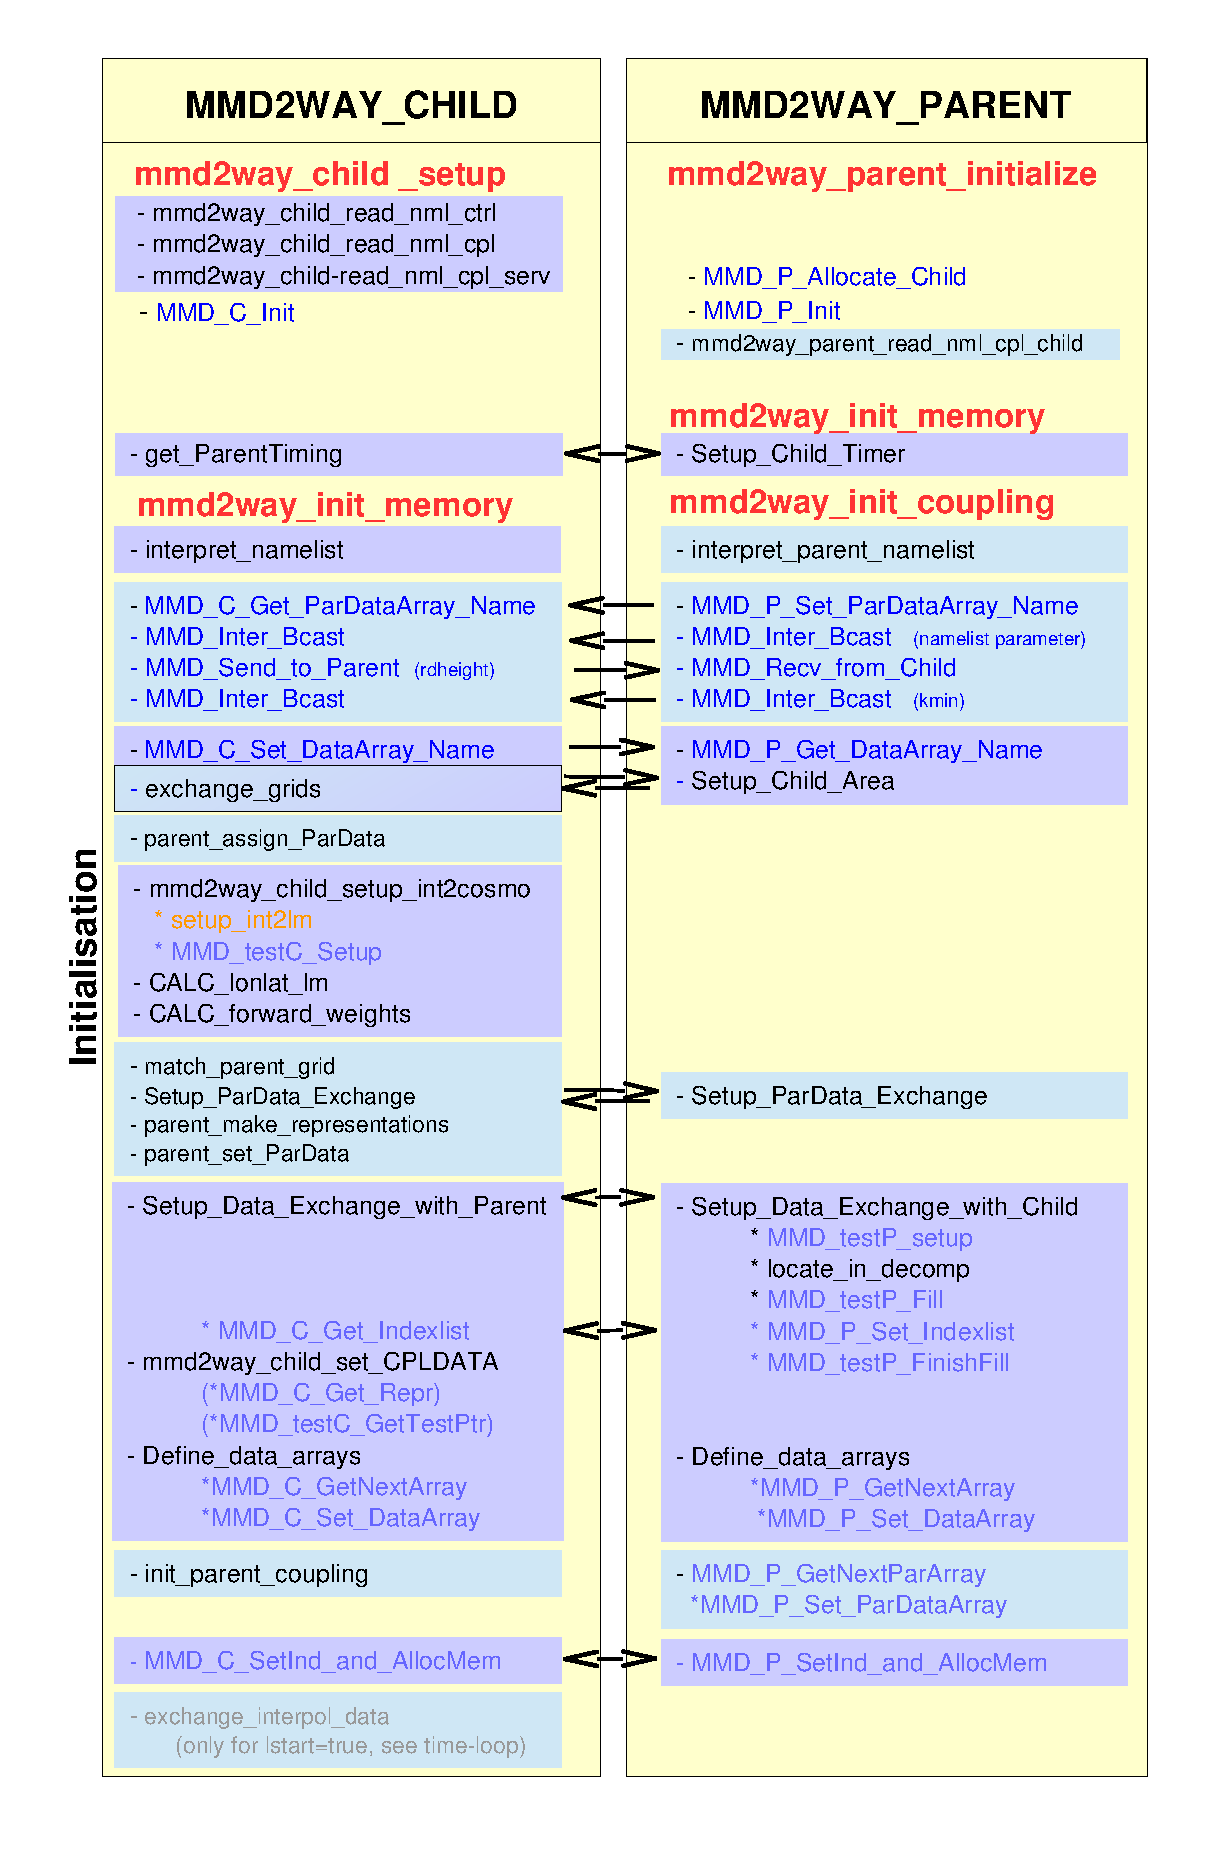
\includegraphics[height=0.9\textheight]{MMDUM_flowchart_iniphase.pdf} 
\end{center} 
\vspace{-.8cm}
\caption{Call sequence of the 2-way on-line coupling routines in the
parent and child submodels in 
ECHAM5/MESSy ($\rightarrow$ COSMO/MESSy)$^n$ in the initial phase:
 Colour code of subroutine names:  the MESSy entry points directly called by
 {\tt messy\_main\_control}: red; MMD library routines: blue; original
 INT2LM routines: orange. The dark blue and light blue boxes indicate
 subroutine calls required for child-to-parent (1-way) and
 the parent-to-child coupling, respectively.
 Arrows indicate the direction of the data exchange between child and parent.} 
\label{fig:call_tree_ini} 
\end{figure*} 
%%%%%%%%%%%%%%%%
\begin{figure*}
\begin{center} 
\vspace{-.3cm}
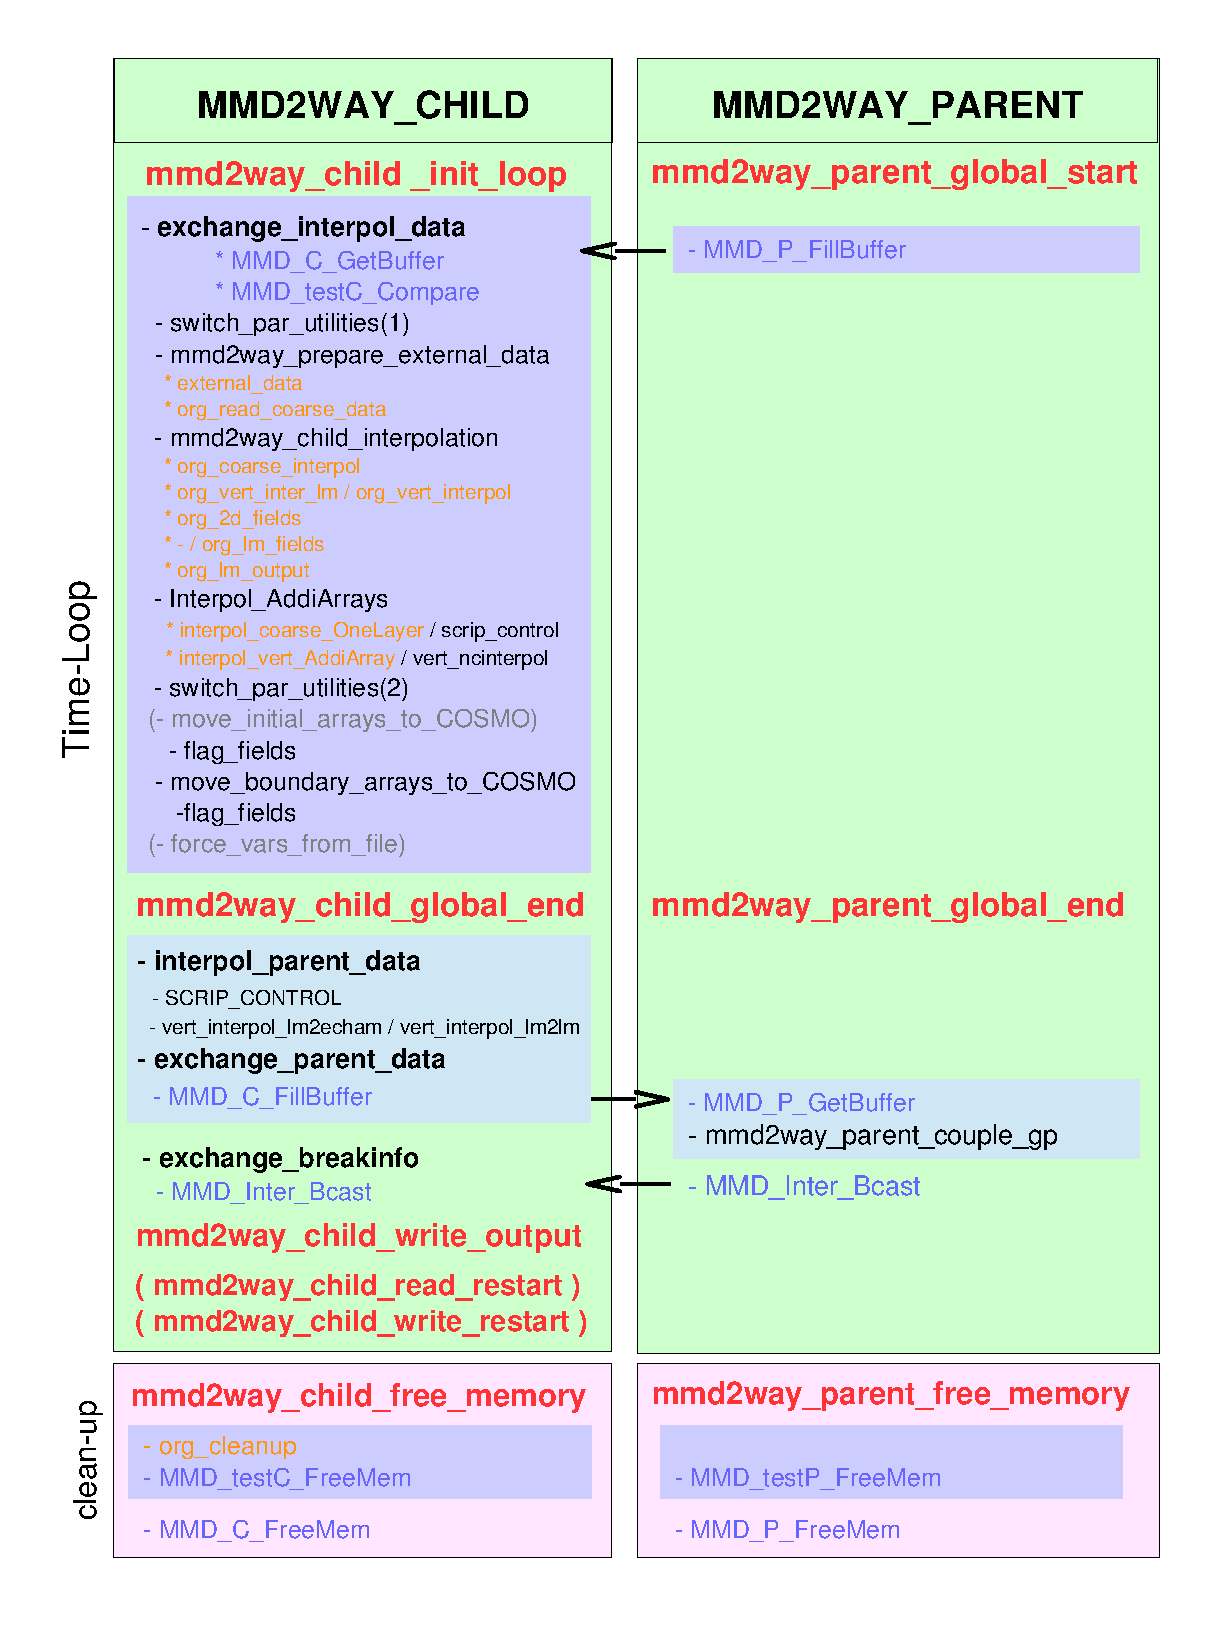
\includegraphics[height=0.9\textheight]{MMDUM_flowchart_timeloop.pdf} 
\end{center} 
\vspace{-.8cm}
\caption{Call sequence of the 2-way on-line coupling routines in the
parent and child submodels in 
ECHAM5/MESSy ($\rightarrow$ COSMO/MESSy)$^n$ during the time loop and
in the finishing phase:
 Colour code of subroutine names:  the MESSy entry points directly called by
 {\tt messy\_main\_control}: red; MMD library routines: blue; original
 INT2LM routines: orange. The dark blue and light blue boxes indicate
 subroutine calls required for child-to-parent (1-way) and
 the parent-to-child coupling, respectively.
 Arrows indicate the direction of the data exchange between child and parent.} 
\label{fig:call_tree_timeloop} 
\end{figure*} 
%%%%%%%%%%%%%%%%

The diagrams in Fig.\ \ref{fig:call_tree_ini}  and Fig.\ \ref{fig:call_tree_timeloop}  sketch the sequence of operations in a coupled simulation.

For the basic coupling of the models, five phases are passed through,
described in the following sections \ref{subMMDsetup} to \ref{subFinPhase}:

\subsection {\bf MMD setup \label{subMMDsetup}} 
Before any submodel specific initialisation takes place, 
the Multi-Model-Driver (MMD) is initialised. 
The MMD library routines setting up the message passing interface
 (MPI) environment are called from the basemodels.
The determination of the model topology and the communicator definition are 
 explained in an extra manual about the MMD library\footnote{The MMD library 
manual is part of the same electronic supplement as this manual.}, 
as these routines work inside the MMD library.
 As model topology, we understand the layout of all parent and child model 
dependencies and the distribution of the models on the available number of 
process entities (PEs) or MPI tasks.

 The topology is determined by the MMD library namelist \verb|MMD_layout.nml|, 
which is written by the run-script \verb|xmessy_mmd| as determined by the user.
The MMD library namelist file \verb|MMD_layout.nml| is read, broadcasted and 
interpreted within the MMD library. All communicators for intra- and
inter-instance 
 communication are determined in accordance to the model topology. 

\subsection{Synchronisation}
To ensure that all instances start, {\it restart} and stop at the 
same date and 
time, the date and time settings of all coupled models need to be synchronised.
This is achieved, if one instance determines the timing of all other instances. 
If in each parent-child model pair the parent dictates the time setup,
 in the end the {\it patriarch} determines the timing of all instances.
Consequently, the TIMER namelist of the {\it patriarch} determines the 
time setup of all child instances. However, it is important to note,
that only the date and time are synchronised, but each model instance uses its
own time step length. 

\subsubsection{Exchange of stop and {\it restart} triggers \label{sec:restarttriggers}}
To ensure the synchronisation of the models, information is 
exchanged during the integration phase of the simulation, whether the simulation is to be interrupted. Such an exchange is 
necessary,
as, apart from the scheduled {\it restart}, exceptional simulation 
interruptions are
triggered, e.g., by QTIMER, when the available scheduler time is consumed. 
Table \ref{tab:logswitches} lists the {\footnotesize LOGICAL} variables, which
determine the behaviour of the simulation.
\begin{table} 
\begin{center}
\caption{{\footnotesize LOGICAL} switches determining the {\it restart}
 behaviour.\label{tab:logswitches}}
{\blockcode
\begin{tabular}{lp{10cm}}\hline
switch & description (if {\tt .TRUE.}) \\ \hline
{\tt lbreak} & interruption or stop of model simulation\\
{\tt lstop}  & stop of model simulation\\
{\tt l\_rerun} & write restart files \\
{\tt l\_TRIGGER\_RESTART} & force model interruption\\
\hline
\end{tabular}
}
\end{center}
\end{table}

For the synchronisation, an exchange of this information has to take place
every parent model time step. The timing of the data exchange is realised by
an {\it event}. The so-called \verb|BREAK_EVENT| is set up in the child model
triggering for each parent model time step the exchange of the required
 {\footnotesize LOGICALs}. If the {\it event} is  
scheduled, the subroutine \verb|exchange_breakinfo| is called.
The parent model sends the contents of its TIMER {\footnotesize LOGICALs} 
\verb|lbreak|, \verb|l_rerun| and \verb|lstop|, 
via the MMD library routine \verb|MMD_Inter_Bcast|. As this subroutine is not
overloaded for {\footnotesize LOGICALs}, these are transferred as 
{\footnotesize INTEGERs}:  \verb|.TRUE.| is 1 and  \verb|.FALSE.| is 0.
\verb|lbreak| indicates, if a simulation is going to be interrupted, 
\verb|lstop| shows, if the simulation will be stopped and 
\verb|l_rerun| signals, if restart files shall be written at the end of the 
time step.

 The contents of the parent models \verb|lbreak| and \verb|l_rerun|
switches are directly written to the respective child model switches. 
There is only one case, which requires more thoughtful action:
if the parent \verb|lstop|-switch is \verb|.TRUE.|, this indicates that the
model simulation is going to be terminated. But in most cases, the
child model uses a shorter time step than the parent model. In this
case, the child models \verb|stop_date| is not yet reached and the
child model must not directly trigger a {\it restart} and exit, but
rather continue the simulation until the \verb|stop_date| is reached. 
Thus, if the parent indicates the end of the simulation, the
variable \verb|lServstop| is set \verb|.TRUE.|, indicating, that the
parent model terminates the simulation. If the child model itself
does not yet indicate the end of the simulation (i.e., \verb|lstop = .FALSE.|),
\verb|lbreak| will be reset to \verb|.FALSE.|, to allow  the child
model to continue its calculation until the \verb|stop_date| is reached.


Additionally, if \verb|lbreak|  is \verb|.TRUE.|,
\verb|l_rerun| and \verb|L_TRIGGER_RESTART| are set \verb|.TRUE.|.
Table \ref{tab:logrestart} lists the settings of the respective {\footnotesize
LOGICALs} of the child model dependent on the status of the parent
model. 
\begin{table} 
\begin{center}
\caption{Setting of child model {\footnotesize LOGICALs}, which
 determine the {\it restart} behaviour. If the simulation is being
 terminated (parent status ``stop'') 
{\tt lbreak} and {\tt l\_stop} of the child model are usually set {\tt
.FALSE.}. Only if the parent and the child model use the same time
step length, {\tt lbreak} and {\tt l\_stop} are also  {\tt .TRUE. }
for the child model.\label{tab:logrestart}}
\vspace*{0.2cm}
{\blockcode
\begin{tabular}{llll}\hline
parent status & {\tt lbreak}  & {\tt l\_rerun}  & {\tt l\_stop} \\ \hline
continue & {\tt .FALSE.} &  {\tt .FALSE.} &  {\tt .FALSE.}  \\
write restart file, continue & {\tt .FALSE.} &  {\tt .TRUE. } &  {\tt .FALSE.}  \\
restart  & {\tt .TRUE. } &  {\tt .TRUE. } &  {\tt .FALSE.} \\
stop     & {\tt .FALSE. (.TRUE.)}  &  {\tt .TRUE. } &  {\tt .FALSE. (.TRUE.)} \\
\hline
\end{tabular}
}
\end{center}
\end{table}

\subsection{\bf Data exchange initialisation}
Different types of data are exchanged between the parent and the child model
and vice versa. While each model requests the data required for the forcing of
the same model, the child model determines the timing of the forcing. Note:
the frequence of the data transfer of the parent-to-child coupling is always 
equal to the frequence of the child-to-parent coupling.
\begin{itemize}
\item  In contrast to the time settings of the instances, the timing
of the data exchange during the coupling process is completely
controlled by the child instance, i.e.,
 the child namelist \verb|&CPL_CHILD| determines the frequency of the data 
exchange for all exchanged data.

\item Each model instance requests the data from its remote model, i.e.,
\begin{itemize}
\item  the child model instances request data for their specific model
domain from the parent model. The child model namelists \verb|&CPL_CHILD_ECHAM|
or \verb|&CPL_CHILD_COSMO| determine  which data fields are exchanged. 
These requests are processed by the parent model during the initialisation phase. 
\item the parent model instances request the required data from their
children according to the \verb|&CPL_PAR_CHILD| namelists (see
Sect.\ \ref{sec:cplparchild}). 
Note, that from each child model instance different data fields can be
requested. If the same {\it target fields} are named and the child domains
overlap, the child data is applied successively from each child model,
giving the last coupled child the highest weight in determining the new value of
the {\it target field}.
These requests are processed by the child models during the initialisation
phase. 
\end{itemize}

\item The child and the parent acquire {\footnotesize POINTER}s to the
data  fields required for the data exchange and (in a child instance) for
the interpolation. 
\item Additionally, the buffers for the data exchange are allocated within the
MMD library. 
\end{itemize}

\subsection{\bf The data exchange}
 During the time loop or the integration phase the {\it exchange fields}
are made available by the parent submodel MMD2WAY\_PARENT (subroutine 
\verb|MMD_P_FillBuffer|). These fields are copied by the child instance
(subroutine \verb|MMD_C_GetBuffer|) and interpolated according to the namelist
settings. 
 Afterwards, the child instance interpolates the data requested by the parent
instance to the parent grid and sends these fields using the MMD library
 subroutine \verb|MMD_C_FillBuffer|. 
Finally, these fields are copied by the parent model using the MMD library
subroutine \verb|MMD_P_GetBuffer|. 

\subsection{\bf Finalisation phase\label{subFinPhase}}
 At the end of the integration coupling specific memory is deallocated.


%+++++++++++++++++++++++++++++++++++++++++++++++++++++++++++++++++++++++++++
%+++++++++++++++++++++++++++++++++++++++++++++++++++++++++++++++++++++++++++
%+++++++++++++++++++++++++++++++++++++++++++++++++++++++++++++++++++++++++++
\section{Coupling of a child model instance to a parent model instance
(1-way, child-to-parent coupling) \label{sec:c2p}}
In case of a regional model instance driven by a parent model
instance, data exchange in the 
direction from the parent to the child model is indispensible.
Initial and boundary data for all prognostic variables and initial data for
additional fields are required. Therefore, this section is dedicated to the
1-way data exchange between the parent and the child instance, as required for a
simple 1-way coupling. First, the program flow on the child side and
afterwards on the parent side are discussed.

\subsection{The child instance}\label{sec:Client}

For the child, the MMD2WAY submodel MMD2WAY\_CHILD provides everything
required for the coupling of the child model to the parent model.
All information required during the coupling process are contained within the
variable \verb|CplData|, which {\footnotesize TYPE} is a Fortran95 structure 
(\verb|T_C_COUPLE_DATA|) and which is allocated to the actual number of 
{\it coupling fields}.

\begin{verbatim}
  TYPE PTR_4D_ARRAY
     REAL(DP), DIMENSION(:,:,:,:), POINTER :: PTR => NULL()
  END TYPE PTR_4D_ARRAY

  TYPE CHAOBJ_NAMES
     CHARACTER(LEN=STRLEN_CHANNEL)    :: CHA = '' ! CHANNEL NAME 
     CHARACTER(LEN=STRLEN_OBJECT)     :: OBJ = '' ! OBJECT  NAME 
  END TYPE CHAOBJ_NAMES

  TYPE T_C_COUPLE_DATA
     ! CHANNEL AND CHANNEL OBJECT NAMES IN PARENT AND CHILD   
     TYPE(CHAOBJ_NAMES)                    :: PARENT
     TYPE(CHAOBJ_NAMES)                    :: CHILD
     ! ORDER OF AXES IN REPRESENTATION ('X','Y','Z','N')
     CHARACTER(LEN=4)                      :: AXIS= '' 
     ! DIMENSION LENGTH
     INTEGER, DIMENSION(4)                 :: ldimlen=0 
     ! INTERPOLATION METHOD (only valid for arrays not included in vartab)
     ! 1.CHAR 'Q' quadratic; 'L': linear; 'M' match interpolation;
     !        'C' conservative remapping 
     ! 
     ! 2.CHAR if 'T' positive definiteness  is required
     ! 3.CHAR if 'T' monotonicity           is required
     ! 4.CHAR if 'V' vertical interpolation is required
     !        if 'W' vertical interpolation via NCREGRID is required (only
     !               possible with 'C' horizontal interpolation and only for
     !               additional fields
     CHARACTER(LEN=4)                      :: C_INTERPOL
     ! INPUT FIELD DELIVERED BY MMD
     REAL(DP), POINTER, DIMENSION(:,:,:,:) :: ptr_in  => NULL()
     ! INTERMEDIATE FIELD OF INT2COSMO
     REAL(DP), POINTER, DIMENSION(:,:,:,:) :: ptr_i2c => NULL()
     ! POINTER(S) TO COSMO/MESSy FIELD(S): DIMENSION == number of time levels
     TYPE(PTR_4D_ARRAY), DIMENSION(:), POINTER :: cosmo => NULL()
     ! POINTER TO COSMO/MESSy BOUNDARY FIELDs: 
     !  (DIMENSION IS ALWAYS TWO FOR THE TWO BOUNDARY LAYER TIME LEVELS)
     TYPE(PTR_4D_ARRAY), POINTER, DIMENSION(:) :: cosmo_bd => NULL()
     ! RANK OF CHILD FIELD (WITHOUT TIME LEVEL DIMENSION)
     INTEGER                               :: rank        = 0 
     ! INDICATOR, IF FIELD IS IN VARTAB
     LOGICAL                               :: lvartab     = .FALSE.
     ! NAME OF VARIABLE IN VARTAB
     CHARACTER(LEN=10)                     :: vartab_name = ''
     ! INDEX OF FIELD in var_lm
     INTEGER                               :: vartab_idx   = 0
     ! INITIAL FIELDS REQUIRED ?
     LOGICAL                               :: L_INITIAL   = .FALSE.
     ! BOUNDARY FIELDS REQUIRED ?
     LOGICAL                               :: L_BOUND     = .FALSE.
     ! INPUT FIELD REQUIRED ?
     LOGICAL                               :: L_INPUT     = .FALSE.
     ! NAME OF REPRESENTATION 
     CHARACTER(LEN=STRLEN_MEDIUM)          :: C_REPR      = '' 
     ! Number of parent field (requested for shortcut test)
     INTEGER                                 :: scn = -99
  END TYPE T_C_COUPLE_DATA
  TYPE (T_C_COUPLE_DATA), DIMENSION(:), ALLOCATABLE :: CplData
\end{verbatim}

This structure contains 
\begin{itemize}
\item the {\it channel} and {\it channel object} names of the 
{\it exchange fields} for the parent model (\verb|TYPE(CHAOBJ_NAMES) :: PARENT|) and
\item   the {\it channel} and {\it channel object} names
for the child model (\verb|TYPE(OCHOBJ_NAMES) :: CHILD|). 
\item information about the {\it dimensions} of the fields:
\begin{itemize}
\item The {\it axis string} (\verb|AXIS|) 
indicates the order of the 'X', 'Y', 'Z' and 'N' direction, and 
\item \verb|ldimlen| contains the length of these four 
{\it dimensions}\footnote{These are
properties already defined and provided by the CHANNEL submodel. See the CHANNEL
manual available in the electronic supplement of \cite{Joeckel10a} for further
information.}.
\end{itemize}
\item \verb|C_INTERPOL| is the flag specifying the
interpolation method. 
\item The structure contains four {\footnotesize POINTERs} or 
{\footnotesize \it POINTER ARRAYs} for the access to the different data fields 
during
the interpolation procedure and to the {\it target fields}. Depending on the
source ({\it exchange field} or from external data) and the {\it target field}
(i.e., {\it boundary} or {\it initial} and {\it input fields}) not all four
{\footnotesize POINTERs} or {\footnotesize \it POINTER ARRAYs} are used for all
{\it coupling fields}\footnote{Note: the different meaning of the different 
fields: \begin{itemize}
\item {\it exchange fields} are those fields exchanged with the parent, they 
are not necessarily associated to a {\it target field}, as they might also be
required for the interpolation and not as input for the child model.
\item {\it coupling fields} are all those fields contained in the variable 
{\tt CplData}, i.e., either {\it exchange fields} or fields additionally provided
by INT2COSMO, e.g., calculated from the external data.
\item {\it target field} can be an {\it input} or 
{\it initial field}, or the respective {\it boundary field} for prognostic 
variables.
\end{itemize} 
The meaning of the individual fields is clarified within the remainder of the 
child description and in the glossary.}:
\begin{itemize}
\item  The first {\footnotesize POINTER} (\verb|ptr_in|) is used for
the {\it in-fields}, i.e., the raw data sent from the parent model.
\item The second {\footnotesize POINTER} (\verb|ptr_i2c|) is associated to the 
{\it intermediate fields}
generated by the horizontal (and vertical) interpolation within INT2COSMO. 
\item The {\footnotesize \it POINTER ARRAY} \verb|cosmo| is associated 
with the {\it target field} in the COSMO/MESSy model. For prognostic variables 
the dimension of the {\footnotesize \it POINTER ARRAY} is given by the number of 
time levels. Each of the {\footnotesize POINTERs} in the 
{\footnotesize \it POINTER ARRAY} is associated to one time level of the 
{\it target 
field}. For diagnostic variables the array dimension is always 1.

\par\noindent For instance,
the prognostic field for the temperature in COSMO is dimensioned by the three
space dimensions and a time level dimension. Depending on whether a two or three
time level integration scheme is used, this fourth dimension is 
allocated to 2 or 3. All time levels have to be made accessible in MMD2WAY\_CHILD
for the respective {\it target field}. Thus the {\footnotesize \it POINTER ARRAY}
\verb|cosmo| is also dimensioned according to the number of the time levels
required by the integration scheme. This yields the {\footnotesize POINTER}s 
 \verb|CplData(ii)%cosmo(nt)%ptr|, where \verb|nt| is an index ranging from 1 to
the number of time levels used in the COSMO model, allowing to access the 
different time levels of the {\it target field}. Thus, \verb|nt| is one of the
time level indices \verb|nnew|, \verb|nnow| and \verb|nold|, respectively.  
 In contrast, a diagnostic variable does not
 depend on the integration scheme, thus one {\footnotesize POINTER} is
sufficient to access a diagnostic {\it target field}. 

\item If boundary data is required for a field, the 
{\footnotesize \it POINTER ARRAY} \verb|cosmo_bd| is allocated to a length of 2
 according to the two time levels
required for the boundary data in the COSMO/MESSy model.
 Each of the {\footnotesize POINTERs} is associated to one
level of the boundary data array.
\end{itemize}
\end{itemize}

To actually perform the coupling, additional information is required: 
\begin{itemize}
\item The \verb|rank| of the field,
\item  the information, if a field is part of the variable 
table in INT2COSMO ({\footnotesize LOGICAL }\verb|lvartab|), i.e., if the
field is an {\it INT2COSMO inherent field},
\item  the name in the variable table 
(\verb|vartab_name|), if \verb|lvartab = .TRUE.|, and 
\item the index of the variable in the variable table of INT2COSMO 
(\verb|vartab_idx|), if \verb|lvartab = .TRUE.|,
\item the {\footnotesize LOGICALs} 
\verb|L_INITIAL|, \verb|L_BOUND| and \verb|L_INPUT| indicating if initial,
boundary or input data is required, and 
\item  the string  \verb|C_REPR|. 
\end{itemize}
The meaning of these variables was already illustrated in the section about the
namelist (Sect.\ \ref{sec:namelist}) and will become clearer in the remainder
of the child model description.


\subsubsection{Initialisation Phase}
The main entry point for submodel initialisation in MESSy is 
\verb|messy_initialize|. In contrast to this, MMD2WAY\_CHILD uses an even
earlier entry point, i.e., \verb|messy_setup|.
% (compare Fig.\ \ref{fig:call_tree}).  
This is necessary, as 
the {\it patriarch} determines the date und time
setup, of all instances in the cascade, which is performed very early during the
 model setup. Thus a very early entry point for MMD2WAY was required.
The second entry point used from the MESSy infrastructure
is \verb|messy_init_memory| in which the INT2COSMO setup is completed, all
required data is allocated and the first coupling is performed. 


\paragraph{\tt \bf mmd2way\_child\_setup: \\} 
This subroutine performs the basic setup of MMD2WAY\_CHILD and defines the
date and time setup of the child instance.
\begin{itemize}
\item {\tt \bf Setting of model wide variables:}
 At the beginning two {\footnotesize LOGICALs} need to be set,
 which determine the information flow in the basemodel and the MESSy generic 
submodels:
\begin{itemize}
\item The {\footnotesize LOGICAL} variable \verb|L_IS_CHILD| defined in 
\verb|messy_main_data_bi| is set 
\verb|.TRUE.|. It is used in the COSMO model itself to 
 switch off certain parts of the code dealing with the import of initial and 
boundary data (in \verb|src_input.f90|).
\item 
\verb|lforcedtime| is required for the 
synchronisation of the parent and child
model instances. Setting  \verb|lforcedtime| = \verb|.TRUE.| prevents
 the calculation of the trigger of the {\footnotesize RERUN} {\it
 event} \verb|l_rerun| in \verb|timer_global_start|. 
If \verb|l_rerun| would be determined in the child instances TIMER itself,
 the child model could finish unnoticed by the parent model and a dead lock in
 MPI would occur resulting in a model hang up.
\end{itemize}

\item {\tt \bf Namelist input:} Subsequently, the MMD2WAY\_CHILD namelists are read and the
content is written to the log-file. 
\begin{itemize} 
\item First, the \verb|&CTRL|-namelist is read in subroutine 
\verb|mmd2way_child_read_nml_ctrl|.  

The \verb|&CTRL|-namelist contains five entries. One switch, which
forces the original output of int2lm to be written
(\verb|l_I2Cori_output|) and the respective {\it event}
(\verb|WRITEI2C_IOEVENT|) determining the frequency of this
output.
The additional three variables define whether (\verb|l_forcevars|)
certain variables (\verb|forcevars|) should be overwritten at the
start of a new model simulation. This is required, e.g., for a more
comprehensive soil moisture initialisation. \verb|forcefile| provides
the path and the filename of the file containing the data required for
this procedure (see Sect.\ \ref{sec:nmlctrl}).


\item Second, the \verb|&CPL_CHILD|-namelist is read in subroutine 
\verb|mmd2way_child_read_nml_cpl|. This namelist defines the
two \verb|IO_TIME_EVENT|s  \verb|CPL_IOEVENT|
and \verb|READEXT_IOEVENT|  scheduling the coupling dates and the
dates at which new external data should be read (see
Sect.\ref{sec:nmlcplchild}). 

\item  Third, the parent model specific coupling
 namelist (\verb|&CPL_CHILD_ECHAM| or \verb|&CPL_CHILD_COSMO|, see
 Sect.\ \ref{sec:nmlcplchildEorC}) is read in the
 subroutine \verb|mmd2way_child_read_nml_cpl_serv|.  
Whether the ECHAM5/MESSy or the COSMO/MESSy specific namelist is read, is 
determined with the help of the MMD library function \verb|MMD_C_GetParentType| 
(located in \verb|mmd_child.f90|).
\end{itemize}
As reading and printing is performed by one task only, the namelist
content is broadcasted to all tasks afterwards.

\item {\tt \bf  Initialisation of MMD library:}
In addition to the child submodel setup, the child model part of the MMD
library  has to be initialised. This is done by the MMD library routine 
\verb|MMD_C_Init|. 
Within this subroutine the C-language group communicators are
determined and the number of PEs covered by the parent model
is retrieved. Variables of the MMD library internal information structure
 (named ``\verb|Me|''), of which the dimensions depend on the number of
 parent PEs are  allocated within 
\verb|MMD_C_Init|\footnote{The MMD library routines are described in detail
in the MMD library manual, which is part of the same electronic
supplement as the MMD user manual.}.

\item {\tt \bf Adjustment to parent time setting:}
To get a meaningful simulation, the time and date setups of the
coupled instances need to be  
synchronised. To achieve this, two important informations are
exchanged between the child and the parent in the
subroutine \verb|get_ParentTiming|: 
\begin{itemize}
\item[1.)] The coupling interval determined in the child
namelist \verb|CPL_CHILD| is sent to the parent model:\\
In the subroutine \verb|get_ParentTiming| first the time interval
of the coupling {\it event} \verb|CPL_IOEVENT| is converted into seconds, as 
this is 
the unambiguous unit to exchange between the two models. The number of 
seconds equivalent to the coupling interval is sent to the parent, which 
accordingly defines a coupling {\it event}. If the coupling interval is not a 
multiple of the parent model time step length the simulation is terminated. 

\item[2.)] The parent model sends the complete date and time settings to the child model in 
order to initialise the date and time of the child basemodel:\\
The  \verb|current_date|, 
the \verb|resume_date|, the \verb|start_date| and the \verb|stop_date| 
are sent from the parent to the child.
The child re-initialises its date settings according to the parent
 dates.  However, the following has to be taken into account:
\begin{itemize}
\item If the child simulation is starting 
(\verb|lstart=.TRUE.|), the child's \verb|start_date| is set to the 
\verb|resume_date| of the parent model. This is done, as it is possible, that
the parent performs a {\it restart}, while the child is
started for the first time.  
 Note that, if \verb|lstart| is also \verb|.TRUE.| for the
parent, the \verb|resume_date| and the \verb|start_date| are
equal anyway.  The \verb|current_date| of the parent is copied
to the \verb|current_date| of the child.
\item If the child simulation is continued
(\verb|lresume=.TRUE.|), the \verb|current_date|
is not set at all, as it is set by the TIMER later on anyway. More
important, the child's \verb|resume_date| 
is not identical to the parent model \verb|resume_date|. It needs to
be calculated from the parent model's \verb|resume_date|. This is necessary, as
the restart files for child and parent are usually not output at
the same time:
They both stop after \verb|l_rerun| was set \verb|.TRUE.|, thus the
child's  
\verb|resume_date| is behind the parent's \verb|resume_date| by the
difference of the parent and the child time step lengths. Based on this,
the child's \verb|resume_date| is calculated from the time step
lengths of the two instances and the parent's\verb|resume_date|.
\end{itemize}
The child's \verb|stop_date| is always a copy of the parent's \verb|stop_date|. Additionally, the COSMO variables \verb|hstop|
and \verb|nstop| are calculated.

 The COSMO/MESSy date and time settings and counters are
 re-initialised within the
 subroutine \verb|messy_timer_COSMO_reinit_time| provided 
by \verb|messy_main_timer_bi|.

Additionally to the dates and times, the time step length of the parent is
sent to the child. This is important as the parent time
step sets the interval for the check-pointing. From this information
the so-called \verb|BREAK_IOEVENT| is defined.

Last but not least, the TIMER-Manager needs to be initialised in case
of a new simulation (\verb|lstart = .TRUE.|) at this point, directly after the
date and time setting.
\end{itemize}
\end{itemize}


\paragraph{\tt \bf mmd2way\_child\_init\_memory\\}


The second part of the initialisation takes place
in \verb|mmd2way_child_init_memory|, 
as the memory allocation and field definitions are to be conducted here.
\begin{itemize} %%i1+
\item {\bf Initialision of \textit{events}:} Due to technical reasons, the {\it events} themselves can not be 
initialised before the MESSy entry point \verb|messy_init_memory|. Thus first of
 all, the four TIMER {\it events} 
\begin{itemize} 
\item[ (i)] for the coupling (\verb|CPL_EVENT|),
\item[(ii)] for reading the external data (\verb|READEXT_EVENT|),
\item[(iii)] for the output interval of INT2LM original output
 (\verb|WRITEI2C_EVENT|)  and 
\item[(iv)] for the check-pointing
 (\verb|BREAK_EVENT|)
\end{itemize}
 are initialised. 
The \verb|BREAK_EVENT| is used to encounter every parent time
 step, whether the 
simulation is interrupted at the end of the time step.  This is inevitably 
necessary to ensure that the parent and the child are interrupted  at
 the same time.  
Otherwise, if the check-pointing information would not be exchanged each parent
time step, one instance hangs up in MPI communication, because the
other instance was interrupted and does not answer the MPI calls anymore.
This implies that the parent time step length needs to be a multiple
of the child time step length.

\item {\bf Namelist interpretation:} After these preparations, the
 contents of the MMD2WAY\_CHILD namelist are 
 interpreted. The subroutine \verb|interpret_namelist| serves two purposes:
\begin{itemize} %%i2+
\item The wildcards in the child {\it channel object} names are analysed
and translated into individual {\it exchange fields}.

For the tracer channel \verb|tracer_gp| two exceptions are made from
the general application of the wildcards:
\begin{itemize}
\item The tracers defined by the COSMO model itself (i.e., the humidity / water
variables), are not requested
from the parent model and have to be listed individually;
\item If ECHAM is the parent model, the liquid and ice tracers (usually
defined by SCAV) are automatically omitted.
\end{itemize}
\item The namelist settings for the {\it mandatory fields} are 
cross-checked with the COSMO variables \verb|yvarini| and \verb|yvarbd|:\\ 
The {\footnotesize LOGICALs} 
\verb|L_INITIAL| and \verb|L_BOUND| are set \verb|.TRUE.|, if the field is 
required by the COSMO model. Furthermore, fields listed in \verb|yvarini| 
or \verb|yvarbd|, but not in the coupling namelist, are added to the variable \verb|CplData|. These are 
data fields, which are calculated by INT2COSMO, but do not require
 direct input from the parent. Examples are the external parameters
 root depth, leaf area index or orography.
Note: {\it mandatory fields} requiring an input field from the parent
model, have to be listed in the namelist. Otherwise the information about the 
{\it channel} and {\it channel object} names in the parent model are missing.
\end{itemize}%%i2-
The settings for the INT2COSMO {\it inherent fields} can partly be
overwritten by the namelist settings in \verb|CPL_CHILD_XXX|. Later on in the
subroutine \verb|mmd2way_child_set_CplData| the interpolation flags set in the
vartab of INT2COSMO are overwritten, if interpolation flags are given in the
  \verb|CPL_CHILD_XXX|. In this way, the INT2COSMO  {\it inherent fields} can
also be horizontally remapped by conservative remapping using SCRIP (flag 'C')
 or vertically transformed by NREGRID (flag 'W').


\verb|CplData| contains data of different sources. The first part of 
\verb|CplData| stems from the namelist and lists the {\it exchange fields},
i.e., 
 fields that are provided by the parent. During the namelist interpretation
other fields are added to \verb|CplData|. These fields are calculated by 
INT2COSMO and are required by the COSMO model. 
Both types of fields are summarised by the term {\it coupling fields}.
Therefore, two important numbers
characterising \verb|CplData| are determined during this analysis:
\begin{itemize}%%i2+
\item \verb|NEXCH| is the number of fields that need to be
exchanged with the parent.
\item \verb|NCOPY| is the dimension of the variable \verb|CplData| 
 containing all {\it coupling fields}, i.e., the {\it exchange fields} and
 the ones determined from external data and copied from INT2LM to the
 basemodel variables.
\end{itemize}%%i2-

Additionally, the subroutine \verb|interpret_namelist| checks for the
interpolation methods required. If conservative remapping using SCRIP
or vertical transformation via NREGRID is required, the {\footnotesize LOGICAL }
\verb|l_i2cscrip| is set \verb|.TRUE.|. This variable is used later
on, to determine, if the calculation of the weights for the
conservative remapping is necessary.

At the end of the subroutine \verb|interpret_namelist| the final list
of all \verb|CplData| fields is output to the log-file.

\item {\bf Definition of the test field:}
 The MMD library includes the possibility to test the horizontal grid 
exchange. Therefore a {\it channel object} for the 
\verb|test_array| ({\it channel} name = 
\verb|'mmd2way_child'|, {\it channel object} name =  \verb|'Test_Ar'|) is
created.   

\item {\bf Exchange of field information with parent instance:} 
The information set in the namelist  relevant for the MMD library
 and the parent, i.e.,\ the {\it channel} and {\it channel object} names 
and the {\it representation} of the respective {\it exchange field},
 are forwarded to the  
MMD library using the MMD library subroutine \verb|MMD_C_Set_DataArray_Name|.
The subroutine is called for each of the {\it exchange fields}. 
Within the library, the MMD internal information structure on child and parent
 side are set up within this subroutine and its counterpart 
(\verb|MMD_P_Get_DataArray_Name|) of the parent.
The end of the list is indicated by the presence of the optional parameter
\verb|LastEntry| which must be set \verb|.TRUE.| to end the list.

\item {\bf exchange\_grids:} \label{SR:exchange_grids}
The parent automatically determines the segment of the
parent domain required for the interpolation in INT2COSMO using the
geographical  
information about the child domain. This is provided by the child
within the subroutine  \verb|exchange_grids|. The local fields \verb|rlon|
and \verb|rlat| containing the geographical coordinates of the grid points
are gathered, yielding one non-decomposed field and sent to the parent. 
In addition, the number of {\it exchange fields} is sent to the parent. 
From the geographical information the parent
calculates the size of the domain, which is required to interpolate the
{\it initial} and {\it boundary fields}. The grid definition for the 
 in-coming data fields 
is afterwards sent back from the parent to the child. The child uses this
information to define the {\it in-grid} and consequently determines the
{\it dimensions} / the {\it representation} of the {\it in-fields}
(\verb|ptr_in|).  
The grid definition received from the parent replaces the \verb|&grid_in| 
namelist of INT2LM in case of the
on-line coupling. Consequently, the following (INT2COSMO) parameters 
are defined by the parent and sent to the child:
\begin{itemize}%%i2+
\item {\footnotesize PARAMETERs} describing the (rotated) parent
grid and the type of the soil water content and soil temperature:\\ 
\verb|startlat_tot|, \verb|startlon_tot|, \verb|endlat_tot|, \verb|endlon_tot|,
 \verb|pollat|, \verb|pollon|, \verb|dlat|, \verb|dlon|, \verb|ie_coarse|,
 \verb|je_coarse|, \verb|ke_coarse|, \verb|ke_soil_coarse|, 
\verb|itype_w_so_rel|, \verb|itype_t_cl|\footnote{For further
 details 
 about the namelist parameters see the INT2LM documentation: {\it 
http://www.cosmo-model.org/content/model/documentation/core/cosmoInt2lm.pdf}:
 last access: 11.10.2016}. 

%%For the meaning of these variables see
%% the parent model description Sect.\ \ref{sec:Sinitcpl}

\item  If the parent is a COSMO/MESSy model (\verb|llm2lm = .TRUE.|),  
additionally the
information about the vertical coordinate system and the reference atmosphere
of the parent COSMO model setup  are required: \verb|vcflat|, \verb|p0sl|,
 \verb|t0sl|, \verb|dt0lp|, \verb|delta_t|, \verb|h_scal|, \verb|svc1|,
 \verb|svc2|, \verb|ivctype|, \verb|irefatm|.
\item The vertical coordinates (\verb|vct| for ECHAM5/MESSy as parent and 
\verb|vcoord_in%sigm_coord| or \verb|vcoord_in%vert_coord|, if
 COSMO/MESSy is parent) 
 and the depth of the soil layers (\verb|czmls_in|) are exchanged. 
\item Next, 
the child receives two fields containing the latitude and longitude 
information for the {\it in-fields} (\verb|latitude_in|
and \verb|longitude_in|). 
\item Finally, if ECHAM5/MESSy is the parent,
 the hybrid coefficients for the interface levels
\verb|ak_in| and \verb|bk_in| are set using the vertical coordinate variable 
\verb|vct|, which has already been sent by the parent.
 Subsequently, the hybrid coordinates for the full levels 
(\verb|akh_in| and \verb|bkh_in|) and the differences of the interface level
 hybrid coordinates (\verb|dak_in| and \verb|dbk_in|) are calculated.
If COSMO/MESSy is the parent, all four  coefficients are
calculated by the subroutine \verb|calc_hybrid_coeff|.
\end{itemize}%%i2-

 
\item{\tt \bf mmd2way\_child\_setup\_int2cosmo:\\}
This subroutine performs the setup of INT2COSMO:
\begin{itemize}%%i2+
\item At the beginning some switches originally determined in the INT2LM 
\verb|&CONTRL| namelist are defined:
\begin{itemize} %%i3+
\item The {\footnotesize LOGICALs} indicating the driving model (\verb|lgme2lm|, 
\verb|lec2lm|, \verb|lhm2lm|, \verb|lcm2lm| and \verb|llm2lm|) are set to  
\verb|.FALSE.|; if ECHAM5/MESSy is parent  \verb|lcm2lm| is \verb|.TRUE.|; if a 
COSMO/MESSy model is parent \verb|llm2lm| is \verb|.TRUE.|.
\item The {\footnotesize LOGICAL ARRAYs} \verb|lushift_in| and \verb|lvshift_in|
indicating if and which type of a staggered grid is used for the horizontal 
wind components are set: For ECHAM5/MESSy as parent all entries are 
\verb|.FALSE.|, 
for the COSMO/MESSy model as parent it is: 
\verb|lushift_in = (.TRUE. , .FALSE.)| and \verb|lvshift_in = (.FALSE., .TRUE.)|.
Additionally, the switches \verb|lcm_hgt_coor|
and \verb|lcm_pres_coor| are set \verb|.FALSE.| in both cases.
\end{itemize}%%i3-

\item The INT2COSMO {\footnotesize LOGICAL} variable \verb|linitial| is set 
\verb|.TRUE.| for the first time step of a new or restarted
simulation, as only for this 
time step initial data need to be calculated, which is indicated by 
\verb|linitial| in INT2LM. \verb|lcomp_bound| is another INT2LM switch, 
indicating that boundary data need to be calculated. It is \verb|.TRUE.| except 
for the first time step.

\item Based on the {\it in-grid} definition and the longitudes and latitudes 
of the {\it in-fields}
as received in the subroutine \verb|exchange_grids|, the staggered  longitudes
and latitudes 
(\verb|slongitude_in| / \verb|slatitude_in|) are calculated.
As ECHAM5 does not use a staggered grid, \verb|slatitude_in| and 
\verb|slongitude_in| are set to \verb|latitude_in| and \verb|longitude_in|.

\item Subsequently, the original INT2LM subroutine \verb|setup_int2lm|
is called. 
The same code is processed, apart from the initialisation and decomposition of 
the grid and the initialisation of many namelist parameters, which are determined
 directly by the setup of the COSMO/MESSy model during the on-line coupling
initialisation.
The changes made to the original INT2LM code in order to implement it as
MESSy sub-submodel (i.e.,\ directly coupled to COSMO/MESSy) are described in 
Sect.\ \ref{sec:INT2COSMOcode}.

\item In \verb|setup_int2lm| the INT2COSMO namelists are read, thus
the INT2COSMO {\footnotesize LOGICAL }switch \verb|lbd_frame_cur| is set 
according to the namelist parameter \verb|lbd_frame| after processing 
\verb|setup_int2lm|.

\item Finally, as the local dimensions of the parallel decomposed
{\it in-fields} have been calculated in \verb|setup_int2lm|, the
 MMD \verb|test_array| can be allocated by the MMD library
 subroutine \verb|MMD_testC_Setup| with the corresponding dimensions.
\end{itemize}%%i2-

At this point the initialisation of \verb|INT2COSMO| is complete.

\item {\bf CALC\_lonlat\_lm \\}
This subroutine calculates the (geographical and rotated) longitude and latitude
fields in grid mid points and interfaces for the INT2LM specific grid
(which is larger by one grid box in each direction compared to the
COSMO grid):
\begin{itemize}
\item rotated longitude / latitude field on grid mid points  (\verb|lon_lm|, \verb|lat_lm|)
\item geographical  longitude / latitude field on grid mid points (\verb|geolon_lm|, \verb|geolat_lm|)
\item rotated longitude / latitude field on grid interfaces  (\verb|loni_lm|, \verb|lati_lm|)
\item geographical  longitude / latitude field on grid interfaces (\verb|geoloni_lm|, \verb|geolati_lm|)
\end{itemize}

\item {\bf CALC\_forward\_weights \\}
For MMD v2.0 the conservative remapping via SCRIP for {\it additional
fields} and INT2COSMO {\it inherent fields} as well as the vertical
interpolation via NREGRID (both by calling the generic MESSy submodel
GRID\_TRAFO) have been implemented.
If conservative remapping is required, MMD2WAY\_CHILD needs to
calculate the remapping weights. The
subroutine \verb|calc_forward_weights| performs this calculation by,
\begin{itemize}
\item firstly, defining the {\it in-grid} and the INT2LM intermediate grid as
geo-hybrid grids (see Manual of GRID),
\item secondly, converting the geo-hybrid grids to the data format
required by SCRIP by calling \verb|CALC_SCRIPDATA|, and
\item thirdly, calculating the weights by calling  the
subroutine \verb|CALC_SCRIP_WEIGHTS|.
\end{itemize}
The conservative remapping is invoked by placing 'C' as interpolation
method in the namelist.

\item {\tt \bf Setup\_data\_exchange\_with\_Parent:}
One of the crucial points of the efficient field exchange by MMD is the 
index list, which directly associates for each child model PE the grid points 
of the parallel decomposed {\it in-field} with the grid points 
and PE of the parallel decomposed parent grid.
The index list consists of six entries for each grid point of
the local child model {\it in-grid}\footnote{i.e.,\ the index list consists of 6 entries
per number of coupled grid points: {\tt index\_list(6,number of grid points)}}:
\begin{itemize}%%i2+
\item[1.)] the first horizontal index of the grid point in the local
grid of the parent PE$_p$ ($i_p$)
\item[2.)] the second horizontal index of the grid point in the local
grid of PE$_p$ ($j_p$), 
\item[3.)] the first horizontal index ($i_c$) in the local child model
{\it in-grid},
\item[4.)] the second horizontal index ($j_c$) in the local child model {\it in-grid},
\item[5.)] the process entity (PE$_c$) on which the local child grid point is 
located,
\item[6.)] the parent PE (PE$_p$) on which the respective grid point is 
located\footnote{A more detailed example is provided in the
 MMD library manual, which is part of the same electronic supplement as this
 manual.}.
\end{itemize}%%i2-
This grid association is performed by the parent instance. Thus the
child has to send its grid definition and decomposition to the parent:
\begin{itemize}%%i2+
 \item On each child PE the longitudes and latitudes of the {\it in-fields} 
\verb|latitude_in| and \verb|longitude_in| are written to the local fields
\verb|my_lon| and \verb|my_lat|. 
\item These fields are gathered on one PE in the 
3D fields (\verb|all_lon(nx,ny,nPE)| and 
\verb|all_lat(nx,ny,nPE)|) with \verb|nx|, \verb|ny| number of grid points in
x and y direction and \verb|nPE| number of child PEs. 
\item Finally, the 3D fields are sent
to the parent model for further calculations.
\end{itemize}%%i2-
Due to their structure, the fields
inherently contain the information required to set up the index list. The
third index gives the number of the child model PE and the first and
second index 
are equal to the indices in the local grid of the respective child
model PE, where the point of the given geographical coordinates is located.

After receiving this list, the parent model associates the (local)
source points for  
each local child grid point to its own parallel decomposed grid
and sends back the list containing the sextuples
associating the child and the parent model grid points with each other. 
This list is received and analysed by the child part of the MMD library within 
the subroutine \verb|MMD_C_Get_Indexlist|, which is called at the end of this 
subroutine (compare Fig.\ \ref{fig:call_tree_ini}).

\item {\tt \bf mmd2way\_child\_set\_CplData:\\}\label{srt:get_CPLDATA}
So far, only those parts of the variable \verb|CplData| have been initialised,
which are set by the namelist. In the
subroutine \verb|mmd2way_child_set_CplData| 
the {\footnotesize POINTERs}  and { \footnotesize \it POINTER ARRAYs}
to the data fields are associated or allocated.
Three different types of {\it coupling fields} are distinguished:
\begin{itemize}%%i2+
\item[A)] fields, which require an {\it in-field} from the parent, which 
is remapped and afterwards copied to the {\it initial}, {\it boundary}
 or {\it input field};
\item[B)] fields exchanged with the parent, which have no direct
 target variable: 
one example is the surface geopotential, which is required for the
remapping  
itself, but has no corresponding {\it target field} in the COSMO/MESSy model. 
This is indicated by setting
the corresponding child {\it channel} name to \verb|'#XXX'| (see 
\verb|FIELD(10)| in the \verb|&CPL_CHILD_ECHAM| namelist in
Fig.\ \ref{fig:nmlcplchildecham}); 
\item[C)] fields, which result from the INT2COSMO interpolation/preprocessing
 routines but have no corresponding {\it in-field}. For instance, all external 
data fields as orography, leaf area index and so on.
These fields are located at the end of the \verb|CplData| variable (indices 
\verb|NEXCH+1| to \verb|NCOPY|).
\end{itemize}%%i2-

The subroutine contains one loop over all entries of \verb|CplData|. The 
individual entries are indicated by the loop index \verb|ii| in the following.
The loop is split into five logical units:
\begin{enumerate}%%e1+
\item association / allocation of the \verb|CplData(ii)%cosmo| 
{ \footnotesize \it POINTER ARRAY};
\item association / allocation of the \verb|CplData(ii)%cosmo_bd| 
{ \footnotesize \it POINTER ARRAY};
\item inquiry, if the {\it coupling field} is an {\it INT2COSMO inherent
field}. If 'yes', 
\begin{itemize}%%i2+
\item the structure component \verb|CplData(ii)%lvartab| is set \verb|.TRUE.|,
\item the \verb|CplData(ii)%vartab_name| is set, and
\item the index of the variable in the INT2COSMO variable table 
(\verb|CplData(ii)%vartab_idx|) is set.
\end{itemize}%%i2-
\item association  / allocation of the {\it intermediate fields}
(\verb|CplData(ii)%ptr_i2c|);
\item association  / allocation of the {\it in-fields} 
(\verb|CplData(ii)%ptr_in|).
\end{enumerate}%%e1-

At the beginning of the loop, the {\footnotesize POINTERs} 
\verb|CplData(ii)%ptr_i2c| and 
\verb|CplData(ii)%ptr_in| are NULLIF(Y)ied and the structure components 
\verb|CplData(ii)%rank|, \verb|CplData(ii)%lvartab|,
\verb|CplData(ii)%vartab_name| and  \verb|CplData(ii)%vartab_idx|
 are initialised by the default values \verb|0|, \verb|.FALSE.|, \verb|''| and 
\verb|0|, respectively. 
In the following the allocation or determination of each of the 
above listed \verb|CplData| entries is described in detail:


\begin{enumerate} %e1+ different parts of loop
\item {\bf determine {\tt CplData(ii)\%cosmo}:}\\
This part is skipped for entries with child model {\it channel} name \verb|'#XXX'| as 
this indicates that the {\it exchange field} is only required in INT2COSMO.

For the determination of the memory for the COSMO/MESSy {\it target field} 
(\verb|CplData(ii)%cosmo|) basically two times two different cases (in all
combinations except for B2A2) have to be taken into account:
\begin{itemize} %i2+ 
 \item[A)] The fields can either be 
\begin{itemize}%i3+ 
\item[A1)] diagnostic or
\item[A2)] prognostic,
\end{itemize}%i3-
which require different memory allocation procedures.
\item[B)] The fields  are
\begin{itemize}%i3+ 
\item[B1)] either already allocated by another MESSy submodel or the basemodel
, or
\item[B2)] required to be allocated within the MMD2WAY\_CHILD submodel itself.
\end{itemize}%i3-
\end{itemize} %i2-

%%%%%%%%%%%%%%%%

\begin{figure*}
\begin{center} 
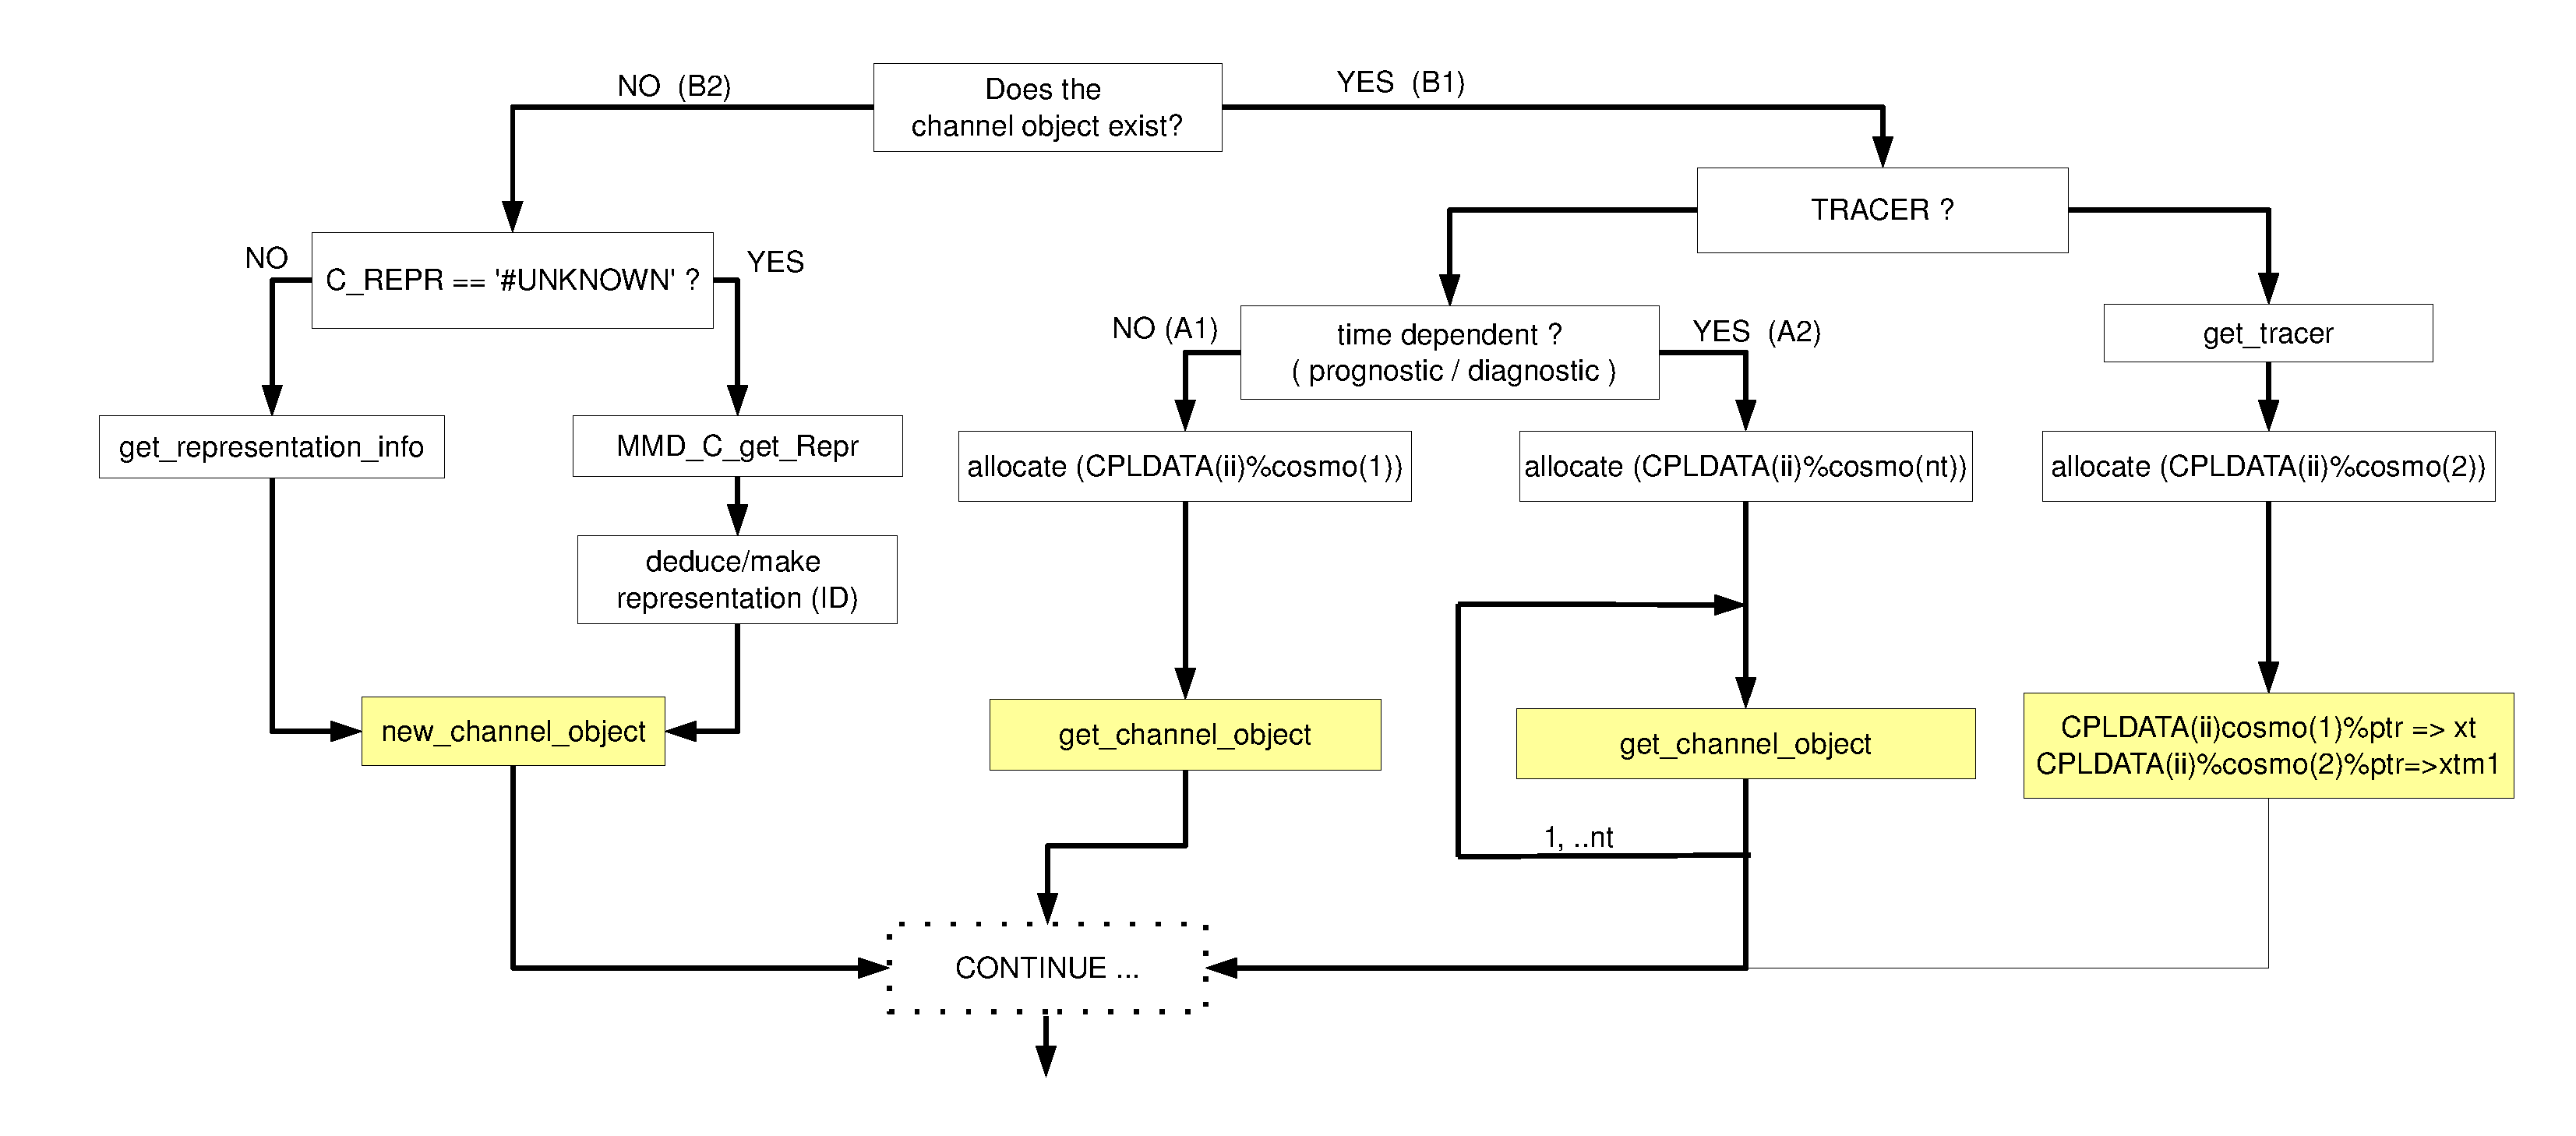
\includegraphics[width=1.02\textwidth]{MMDUM_decisiontree.pdf} 
\end{center} 
\caption{Flow-chart illustrating the association of the {\tt CplData(ii)\%cosmo}
{\footnotesize \it POINTER ARRAY}. The labels in brackets (A1, A2, B1 and B2)
 refer to the respective cases listed in the text. The yellow boxes point to 
those subroutine calls in which the individual {\footnotesize POINTERs} of the
{\footnotesize \it POINTER ARRAY} {\tt CplData(ii)\%cosmo} are finaly associated.} 
\label{fig:A1A2B1B2} 
\end{figure*} 
%%%%%%%%%%%%%%%%
Figure \ref{fig:A1A2B1B2} comprises a flow chart showing the basic procedure
for the association of the \verb|CplData(ii)%cosmo| {\it \footnotesize POINTER
ARRAY}
\begin{itemize} %i2+ 
 \item[Regarding A)] 
The nature of the respective variable (diagnostic or prognostic) determines
the dimension of the { \footnotesize \it POINTER ARRAY} \verb|CplData(ii)%cosmo|:
\begin{itemize} %%i3+
\item[A1)] For a diagnostic variable the dimension is 1, as only one 
{\it target field} exists. 
\item[A2)] For the prognostic variables the dimension equals 
the number of time levels of the time integration
scheme used. For instance, for the leap frog scheme the dimension is 3,
 whereas for a two-time level scheme (e.g.,\ Runge-Kutta) it is 2.
 This is due to two reasons:
\begin{itemize}%%i4+
\item For an integration scheme with more than 2 time levels, more than 1 time 
level needs to be initialised by MMD2WAY\_CHILD.
\item In the COSMO model prognostic variables are allocated with an extra rank
for the time level. For the sake of computational efficiency, 
 the indices indicating the different time levels (\verb|nnew|, \verb|nnew| and
\verb|nold|) are shifted instead of copying the newly integrated value to the 
old field at the beginning of each time step. 
Thus, it is not a priori known which time level (index in the prognostic 
field) is required at a specific point in time. 
Hence, all time levels must be available for the coupling.
\end{itemize}%%i4-
Each of the {\footnotesize POINTERs} of the {\footnotesize \it POINTER ARRAY} 
\verb|CplData(ii)%cosmo| (\verb|CplData(ii)%cosmo(nt)%ptr|, with \verb|nt| being
the index for a time levels) is 
 associated to one time level of the prognostic variable. Thus, the correct
time level can be addressed by the indices (\verb|nnew| and \verb|nnow|) usually
used in the COSMO model to access the correct time levels.
\end{itemize}%i3-

\item[Regarding B)] The child model {\it channel} name includes the
 information, if MMD2WAY\_CHILD
needs to allocate the required memory itself (\verb|'mmd2way_child'| as child 
{\it channel} name in the namelist), or if the {\it target field} is already 
allocated by other COSMO/MESSy submodels or the basemodel (all other cases).
 In the latter case
the {\footnotesize POINTERs} of the \verb|CplData(ii)%cosmo| 
{\footnotesize \it POINTER ARRAY}
 are associated to the already existing memory:
\begin{itemize}%i3+
\item[B1)] The required {\it channel object} exists already:\\
First, the nature of the {\it channel object} is inquired by looking for the 
{\it channel object attribute} \verb|number_of_timelevels| using the CHANNEL 
subroutine \verb|get_attribute|. 
\begin{itemize} %i4+
\item[A1)] If the attribute does not exist, the variable is of
diagnostic nature  
and the {\footnotesize \it POINTER ARRAY} \verb|CplData(ii)%cosmo| is allocated 
to the dimension 1 
 (as only one {\footnotesize POINTER} is required for a diagnostic variable). 

Afterwards, \verb|CplData(ii)%cosmo(1)%ptr| is associated to the respective 
memory by calling
the CHANNEL subroutine \verb|get_channel_object|\footnote{See the CHANNEL manual,
 which is part of the electronic supplement of \citeauthor{Joeckel10a}, 
\citeyear{Joeckel10a}.}.

Then, the rank (\verb|CplData(ii)%rank|) of the field is acquired by calling the 
MMD2WAY\_CHILD subroutine \verb|get_rank|.
In the subroutine \verb|get_rank|, first, the {\it channel object} 
{\it representation ID}
is determined by calling the CHANNEL subroutine \verb|get_channel_object_info|
with the input parameters {\it channel} and {\it channel object} name. 
Second, with the {\it representation ID}, the \verb|rank| of a 
{\it channel object} with this {\it representation} is found out by calling 
\verb|get_representation_info| with the {\it representation ID}
 as input and the \verb|CplData(ii)%rank| as output parameter.

\item[A2)] If the attribute exists, the {\it channel object} is of prognostic
nature and \verb|CplData(ii)%cosmo| is allocated to the number of time levels as
 denoted
by the attribute (\verb|timelev| is the return value of the subroutine 
\verb|get_attribute| containing the number of required time levels).
Afterwards, a loop over the number of time levels is executed associating for
each time level one {\footnotesize POINTER} of the 
{\footnotesize \it POINTER ARRAY}
 to one time level of the {\it target field} using the subroutine 
\verb|get_channel_object|. 
Note: for all prognostic variables individual {\it channel objects} for the 
single time levels must exist. 
Finally, the \verb|CplData(ii)%rank| is determined as in the diagnostic case.

\item[XT)] A special case exists for tracers: \\
In contrast to the prognostic COSMO variables, the tracer structure provides 
individual variables for all time levels\footnote{Detailed information about
 the TRACER submodel are provided by \cite{Joeckel08a}.}, such that the
index rotation instead of the copying of one time level to the other at the
end of one time step is not possible for the tracers. 
Consequently, tracers must be treated differently:
\begin{enumerate}%e2+
\item  First, the tracer index \verb|idt| is inquired by the TRACER subroutine 
  \verb|get_tracer|. 
\item Next, \verb|CplData(ii)%cosmo| is always allocated to 2 and the first 
{\footnotesize POINTER} of the {\footnotesize \it POINTER ARRAY} always points to
the current tracer field \verb|xt| of that specific tracer. The target of
the second {\footnotesize POINTER} depends on the integration scheme. For a 2 
time level scheme it points to \verb|xtm1| and for a 3 level scheme to 
\verb|xtf|.
\item The rank of a tracer is always 3, thus \verb|CplData(ii)%rank| is set to 3 
for tracers and 
\item the flag in the TRACER meta-structure indicating that a tracer is
already initialised (\verb|ti_gp(idt)%tp%meta%cask_i(I_MMD_INIT)|) is set to
\verb|ON| at simulation start (\verb|lstart = .TRUE.|),
otherwise the tracer field would be overwritten by subsequent tracer 
initialisation routines. 
\end{enumerate}%e2-
\end{itemize}  %i4-% diagnostic /prognostic 

\item[B2)] MMD2WAY\_CHILD needs to allocate the memory itself, as no other submodel 
provides the memory for the {\it exchange field}. 
This field is calculated from an {\it in-field} provided by the parent
model and 
supplied to other MESSy submodels (e.g.\ emission fields could be down-scaled
from the coarse grid instead of being directly read in by IMPORT\_GRID).

 If the {\it representation} is named in the MMD2WAY\_CHILD
 namelist (\verb|&CPL_CHILD_ECHAM| or \verb|&CPL_CHILD_COSMO|) and stored
in the structure component \verb|CplData(ii)%C_REPR|, this is an easy task.
The {\it representation} ID \verb|repr_input| and the corresponding rank are 
inquired calling the CHANNEL 
subroutine \verb|get_representation_info|. Knowing the
{\it representation} ID, the new {\it channel object} can be defined
 calling the  
CHANNEL subroutine \verb|new_channel_object|.


But the {\it representation} is not always a priori known. This is indicated in
 the MMD2WAY\_CHILD namelist by setting the {\it representation} string to 
\verb|'#UNKNOWN'|.
 A classical example are emission fields provided as multi-level emissions. 
They are in the \verb|Nx2D|-format \citep[see][]{Kerkweg06a}, i.e., N 
levels 
attributed to different emission heights containing each 2D emission 
information.
 If the number of levels is not a priori known by the child
model, the parent model provides additional information about the
{\it representation}, when the {\it representation} string 
(\verb|CplData(ii)%C_REPR|) is set to \verb|'#UNKNOWN'|. 
MMD2WAY\_CHILD acquires this information by calling the MMD library subroutine
\verb|MMD_C_Get_Repr| which provides the {\it representation} name 
(\verb|par_repr|),
 the {\it axis string} (\verb|par_axis|), the global {\it dimensions}
 (\verb|par_gdimlen|)
and the height {\it attribute} (\verb|par_att|) of the 
{\it exchange field} in the parent model.
Based on this, MMD2WAY\_CHILD determines its own {\it representation}: 
\begin{enumerate}%e2+
\item[i)] If the {\it representation} name is one of \verb|'GP_3D_MID'|, 
\verb|'GP_3D_INT'| or \verb|'GP_2D_HORIZONTAL'| using the same 
{\it representation} names in
the child model automatically leads to the correct result, 
as these are standard {\it representation}s. 
\item[ii)] In case of the {\it representation} \verb|'GP_3D_1LEV'| the 
{\it representation} is converted to \verb|'GP_2D_HORIZONTAL'|.
\item[iii)] In all other cases MMD2WAY\_CHILD has to define a new {\it representation}:
\end{enumerate}%e2-

For the definition of a new {\it representation} 
the {\it dimensions} need to be defined first:\\
This is done by looping over the 4 {\footnotesize CHARACTERS} of the 
{\it axis string} \verb|par_axis|.
Simultaneously, 
\begin{itemize}%i4+
\item[-] the \verb|rank| of the array, 
\item[-] the local dimension length \verb|dim_len| and 
\item[-] the {\it axis string} \verb|dim_axis| 
\end{itemize}%i4-
of the child array are determined. 
For instance, if the \verb|il|'s component of \verb|par_axis| is \verb|'X'|, 
the \verb|rank| is increased by one, 
\verb|dim_ids(il)| is set to \verb|DIMID_LON|,
which is the {\it dimension} ID for the longitude of the child model and 
\verb|dim_len(il)| is set to \verb|ie|, which is the local dimension length for
the COSMO arrays. 

\begin{itemize}%%i4+
\item The horizontal dimensions of the fields are different between the parent 
and the 
child, but are implicitly given by the definition of the COSMO grid. 
Thus for the \verb|'X'| and \verb|'Y'| dimension the sizes are known and the 
 COSMO definitions can be used. 

\item This is different for the \verb|'Z'| and
\verb|'N'| dimensions, which can basically adopt every arbitrary value, but
these dimensions have to be the same in the parent and the child. 
Thus new dimensions are defined for the \verb|'Z'| and \verb|'N'|
dimensions, using the dimensions provided by the server model 
(\verb|par_gdimlen|). 
The newly defined dimensions are named in a generic way:  
\begin{enumerate}%%e2+
\item For the vertical dimension they start with \verb|'DIM_'| followed
by a string containing the number of z-levels, and ending with \verb|'LEV'|.
For instance, when the number of z-levels is 5 this yields the name 
\verb|'DIM_5LEV'|. Before actually defining the dimension, it is tested 
if this dimension exists already.
In this case, the existing {\it dimension} ID is taken. 
This test prevents repeated
definition of the same {\it dimension}. 
\item 
For the number (\verb|'N'|) dimension the same procedure takes place,
only the name of the dimension variable ends with \verb|'N'| instead of 
\verb|'LEV'|.
\end{enumerate}%%e2-
\end{itemize}%%i4-

After the loop over the {\it axis string}, the \verb|rank|, the local {\it axis 
string} and the local dimension lengths have been determined. This allows for
the definition of the {\it representation}:
\begin{itemize}%i4+
\item If \verb|rank| is 2 and the \verb|'Z'| and \verb|'N'| dimension lengths are
 zero, the {\it representation} is equal to the standard {\it representation} 
\verb|GP_2D_HORIZONTAL|. 
\item If the rank is larger than 2 and smaller or equal to 4,
a new {\it representation} needs to be defined, 
\item in all other cases the {\it representation}
cannot be properly evaluated and the simulation is terminated with the error
message \verb|'CANNOT IDENTIFY REPRESENTATION'|.
\end{itemize}%i4-

The ECHAM5/MESSy model uses another order of 
{\it dimensions} as the COSMO/MESSy model. Therefore
the {\it axis string} characters, the {\it dimension} IDs and the 
{\it dimension} lengths must be permutated, if ECHAM5/MESSy is server.
For instance, \verb|dim_axis = 'XZNY'| becomes \verb|dim_axis = 'XYNZ'| and the 
\verb|dim_len| has to be changed accordingly. 

The new {\it representation}s are constructed by the subroutine 
\verb|make_cosmo_representation|. Input to this subroutine are
\begin{itemize}%i4+
\item  the lengths of the \verb|'Z'| and \verb|'N'| dimensions (these are zero 
if the corresponding {\it dimension} is not required), 
\item the {\it dimension} IDs (\verb|dim_ids|), 
\item the {\it axis string} (\verb|dim_axis|),  and 
\item the dimension lengths (\verb|dim_len|). 
\end{itemize}%i4-
Output of the subroutine is the {\it representation} ID  of the newly created 
{\it representation}.
Based on the incoming parameters, the respective {\it representation} is created.
The names of the {\it representation}s are as generic as the {\it dimension} 
names.
If \verb|'Z'| and \verb|'N'| dimensions are required, the {\it representation}
is named \verb|'REPR_4D_zzLEV_nnN'| where \verb|'zz'| stands for the number
of z-levels and \verb|'nn'| for the number of n-levels.
The {\it representation} names for \verb|'Z'|-dimension only or 
\verb|'N'|-dimension only are  \verb|'REPR_3D_zzLEV'| or  \verb|'REPR_3D_nnN'|,
respectively. Using the CHANNEL subroutine \verb|get_representation_info|, it is
 inquired, if the {\it representation} exists already. 
In this case the return variable \verb|reprid| is set to the ID of the
matching {\it representation}, otherwise, the {\it representation} needs to be created
via the channel subroutine \verb|new_representation|.
In both cases the {\it representation} ID is handed back to the calling 
subroutine. After the {\it representation} is identified or newly created,
 the new {\it channel object} of the \verb|'mmd2way_child'| {\it channel} can be 
created as described above for the case 
when the {\it representation} is known a priori. Additionally, a new {\it 
attribute} to the {\it channel object} will be set, if it was sent from the 
parent model(\verb|par_att|). This is required in case of Nx2D emission
 fields,  as the layer heights
have to be known in addition to the amount given by the field itself. 

\end{itemize}  %%i3-% items B1, B2

\end{itemize}  %%i2-% items A,B

\item {\bf Determine {\tt CplData(ii)\%cosmo\_bd}:}\\ %e1
As for \verb|CplData(ii)%cosmo|, this part is skipped, if the child model
{\it channel} name is \verb|'#XXX'|.
If \verb|L_BOUND| is \verb|.TRUE.|, boundary data for the specific {\it coupling
 field} is required. 
In this case \verb|CplData(ii)%cosmo_bd| is allocated to 2, as the boundary
fields always consist of two time levels. In the standard COSMO model, these
contain the fields at the beginning and the end of the time interval for which
the boundary data is valid. During this interval the boundary data is linearly 
interpolated according to the elapsed time. In the on-line coupled setup
the two time levels for the boundary data are filled with the same values.
Otherwise the parent model needs to be run ahead by one boundary data time 
interval, which renders a 2-way nesting impossible. As the on-line
coupling enables and requires much higher coupling 
frequencies, the error of this procedure is small.

Although the levels are filled with the same values and the linear interpolation
in time is not required anymore, the procedure is kept
 in order to leave untouched as much code as possible of the COSMO model.

For a {\it boundary field}, the 4D-{\footnotesize POINTER} to the full 
boundary data field is acquired  with the subroutine \verb|get_channel_object|.
Afterwards, the {\footnotesize POINTERs} of the {\footnotesize \it
POINTER ARRAY} 
 \verb|CplData(ii)%cosmo_bd(1:2)%ptr| are set dependent on the rank of
the data field. For instance,
\begin{verbatim}
 IF ( (CplData(ii)%rank == 3  .AND.  &
  (TRIM(CplData(ii)%CHILD%CHA) /= 'tracer_gp')) THEN
    CALL get_channel_object(status             & 
         , TRIM(CplData(ii)%CHILD%CHA)        &
         , TRIM(CplData(ii)%CHILD%OBJ)//'_BD' &
         , p4=bdptr                            )
         
...

       CplData(ii)%cosmo_bd(1)%ptr =>bdptr (:,:,:,1:1)
       CplData(ii)%cosmo_bd(2)%ptr =>bdptr (:,:,:,2:2)
       NULLIFY(bdptr)
 
\end{verbatim}
For a \verb|rank=3| field the {\it boundary field} has 4 dimensions.
Thus, the first boundary {\footnotesize POINTER} is set to the first boundary 
time level and the second to the second one. 
Note: this procedure does not work for 4D data fields, for  which 
{\it boundary fields}
 would be 5-dimensional. However, a coupling to the individual boundary time 
levels would still be possible (and easily implementable), if required. 
So far such fields are
 not part of the model system apart from tracers.


Tracers are again processed differently. The two time levels of the boundary 
data are {\it channel objects} of the two TRACER CHANNELS \verb|tracer_gp_x001|
and \verb|tracer_gp_x002|. Thus, the { \footnotesize POINTERs} to the boundary 
data can be associated directly by
\begin{verbatim}
 CALL get_channel_object(status             & 
    , TRIM(CplData(ii)%CHILD%CHA)//'_x001' &
    , TRIM(CplData(ii)%CHILD%OBJ)          &
    , p4=CplData(ii)%cosmo_bd(1)%ptr        )
\end{verbatim}

and 
 
\begin{verbatim}
 CALL get_channel_object(status             & 
    , TRIM(CplData(ii)%CHILD%CHA)//'_x002' &
    , TRIM(CplData(ii)%CHILD%OBJ)          &
    , p4=CplData(ii)%cosmo_bd(2)%ptr        )
\end{verbatim}


\item {\bf Determine CplData(ii)\%lvartab, CplData(ii)\%vartab\_name and
  CplData(ii)\%vartab\_idx:}\\%%e1 item
  Some data manipulations require a distinction between
  {\it INT2COSMO inherent field}s and {\it additional field}s. All {\it INT2COSMO inherent fields} are listed in the variable table structure (\verb|var_lm|)
  in INT2COSMO. This table determines -among
  other things- the {\it intermediate} and the {\it in-fields}, as well as the 
  interpolation method. \verb|CplData(ii)%lvartab|, 
  \verb|CplData(ii)%vartab_name| and \verb|CplData(ii)%vartab_idx| are set in a 
  loop over the variable table of INT2COSMO:
  \begin{itemize}%i2+
  \item The structure component \verb|CplData(ii)%lvartab| is \verb|.TRUE.|, if 
  the variable is element of the INT2COSMO variable table.
  \item Additionally, the name of the field in the variable table is stored in 
  the structure component \verb|CplData(ii)%vartab_name|. This is useful 
  especially for one
  variable, the roughness length, as only for this the names (and the meaning)
  of the variables are different in INT2COSMO and in COSMO. In INT2COSMO
  the roughness length is called \verb|'Z0'| whereas the COSMO model treats the
  product of roughness length times gravitational acceleration named 
  \verb|'gZ0'|. These two need to be associated with each other.
  \item Finally, the location, i.e., the index, of the field in the INT2COSMO 
  variable table is stored in the structure component 
  \verb|CplData(ii)%vartab_idx|.
  \end{itemize}%i2-

\item[4./5.] {\bf Determine {\tt CplData(ii)\%ptr\_in} and 
{\tt CplData(ii)\%ptr\_i2c}:}\\ %%e1 item
   The information, if a {\it coupling field} is part of INT2COSMO,
 is required for the association of the {\footnotesize POINTERs} 
\verb|CplData(ii)%ptr_in| and 
   \verb|CplData(ii)%ptr_i2c|.
   If the field is part of the variable table, the memory for the {\it in-field}
   and the {\it intermediate field} have been already allocated in INT2COSMO.
   Otherwise the memory for these fields is allocated in MMD2WAY\_CHILD itself.
   \begin{itemize}%i2+
   \item[a)] The memory for the {\it intermediate} and {\it in-fields} exists 
   already: %% item of i2
\begin{itemize}%%i3+
   \item The {\footnotesize POINTER} \verb|CplData(ii)%ptr_in| can 
    be directly associated calling the subroutine \verb|get_channel_object|. 
    For this call the object name is constructed by adding the
    suffix \verb|_IN| to the {\it target field} name and the name of the 
    {\it channel} is \verb|'MMDC4_IN'|\footnote{One special case has to be 
    considered: the {\it in-field} for {\tt 'W\_SO'} is not necessarily named 
     {\tt 'W\_SO\_IN'}, it can also be  {\tt 'W\_SO\_REL\_IN'}.}.
    When no object is found the simulation will be terminated.
    \item After the {\footnotesize POINTER} \verb|CplData(ii)%ptr_in| is 
    associated, 
    the {\it representation}
     ID of this object is obtained by calling \verb|get_channel_object_info|. 
     \item
     This ID is used to acquire the {\it axis string} (\verb|CplData(ii)%AXIS|) 
     and the local dimensions (\verb|CplData(ii)%ldimlen|). This information is
     required by the MMD library for the data exchange.
     \item Afterwards, \verb|CplData(ii)%rank| is determined dependent on the 
     third dimension of \verb|ptr_in| to be \verb|2| or \verb|3|.
     \item Additionally, the INT2COSMO field is marked as read  
     (\verb|var_in(itab)%lreadin = .TRUE.|). 

     \item The {\footnotesize POINTER} \verb|CplData(ii)%ptr_i2c| to the        
     {\it intermediate field} required in INT2COSMO is
       set by the subroutine \verb|get_channel_object| by using 
      \verb|CplData(ii)%vartab_name| as {\it channel object} name and 
      \verb|'MMDC4'| as {\it channel} name.
\end{itemize}%%i3-

   \item[b)] The memory for the {\it intermediate} and {\it in-fields}
   needs to be allocated ({\it additional fields} only):\\ %%i2 item
   The {\it representation} of the {\it intermediate} and {\it in-fields} is 
   not a priori known. 
   They are determined depending on the \verb|rank| of the field.
   \begin{itemize}%%i3+
   \item For \verb|CplData(ii)%rank = 2| the {\it in-field} and the 
   {\it intermediate field} are defined using the existing {\it representation
   IDs} \verb|REPR_I2C_2D_IN| and \verb|REPR_I2C_2D|, for a 2D
   {\it in-field} and a 2D {\it intermediate field}, respectively. 
    \item If  \verb|CplData(ii)%rank| is \verb|3| and \verb|CplData(ii)%C_REPR| 
    is \verb|'GP_3D_MID'|, the prior defined 
   {\it representation IDs} \verb|'REPR_3D_MID_IN'| and \verb|'REPR_I2C_3D_MID'| 
   are used.
   \item In all other cases, the subroutine \verb|make_i2c_representation| is 
   called with the vertical and number dimensions as input parameters.
    The subroutine determines 
   similarly to the subroutine \verb|make_cosmo_representation| the 
   {\it representation}s for the {\it intermediate field} and the {\it in-field}.
   \end{itemize}%%i3-
    Using these {\it representation}s, the new {\it channel objects}
    for the {\it in-field} and the {\it intermediate field} are defined.
    The {\it channel objects} for the {\it in-fields} are added to the INT2COSMO
    {\it channel} \verb|'MMDC4_IN'|. The {\it intermediate fields} are added to 
    the {\it channel} \verb|'MMDC4'| containing all {\it intermediate fields}.

    Additionally, the {\it axis string} (\verb|CplData(ii)%AXIS|) and the local 
    {\it dimensions} (\verb|CplData(ii)%ldimlen|) are determined by calling the 
    subroutine \verb|get_representation_info| with the {\it representation ID} 
    \verb|REPR_IN|.
 \end{itemize} %%i2-

 \end{enumerate} %e1-% different parts of loop

\item {\tt \bf Define\_data\_arrays:\\}
After all data fields are associated or allocated, the respective 
{\footnotesize POINTERs} of the {\it in-fields} can be forwarded to the
 MMD library routines.
To address the correct {\it exchange fields} within the MMD library, a loop over
the {\it exchange fields} is performed by using the MMD library function 
\verb|MMD_C_GetNextArray|. For each field the MMD library subroutine
\verb|MMD_C_Set_DataArray| is called, handing over the {\footnotesize POINTER}
to the memory allocated for the {\it in-field}.  
Additionally, the {\it axis string} and the local {\it dimension} length are 
communicated to the MMD library, which, internally uses
this information, later on, to unpack the data received from the
parent model.

\item {\tt \bf MMD\_C\_SetInd\_and\_AllocMem\\}
The initialisation is finalised by calling the MMD library subroutine 
\verb|MMD_C_SetInd_and_AllocMem|. It invokes the MMD internal 
calculation of the required buffer sizes and the actual memory allocation
via \verb|MPI_alloc_mem|.

With this the initialisation phase for the MMD2WAY\_CHILD submodel is complete.
\end{itemize} %%i1-

In case of a new start of a simulation (\verb|lstart = .TRUE.|) the
actual data exchange and interpolation is performed at the end
of \verb|mmd2way_init_memory| instead of \verb|mmd2way_init_loop|
during the time integration. This is necessary, as the initialisation
of the fields in the COSMO model needs to take place prior to the time
loop.


\subsubsection{Integration Phase}
The procedure explained in this section is part of the subroutine
\verb|mmd2way_init_loop|, as the update of the child model fields is
required at the very  
beginning of the respective time step. The very first time step of a model 
simulation (\verb|lstart = .TRUE.|) builds an exception to this rule, because
in the very first initialisation not only {\it input} and {\it boundary fields},
 but also the {\it initial fields} are calculated. 
The latter are already used during the 
end of the initialisation phase in the COSMO model. Therefore the very first 
data transfer and interpolation takes already place in 
\verb|mmd2way_child_init_memory|. 
Nevertheless, the procedure explained here is the same.

There are two chunks of information, which need to be exchanged during the
integration phase of a 1-way coupled simulation: the coarse grid data
and the TIMER status of the parent model. For the 2-way coupling, in
addition, the data required by the parent is (after processing)
sent to the parent.

\paragraph{Data exchange, interpolation and supply\\}
First of all, the coupling {\it event} (\verb|CPL_EVENT|) determines,
 if data exchange should occur in this time step. If this is the case, the
MMD2WAY\_CHILD private subroutine \verb|exchange_interpol_data| is called:
\begin{enumerate} %%e1+
\item First, the data exchange is performed by calling the MMD library 
subroutine 
\verb|MMD_C_GetBuffer|, which fills all {\it in-fields} with the updated values 
sent by the parent model.
The subroutine \verb|MMD_C_GetBuffer| also provides a measure for the
time required for coupling. It hands back a variable containing the time
in seconds, 
which the child model had to wait until the parent model data was accessible. 
This information is written to the log-file.
\item
As soon as the {\it in-fields} are filled, the MMD internal check of the 
consistency
of the exchanged horizontal data field is performed. This is invoked by 
calling the subroutine \verb|MMD_testC_compare|. As the content of the 
\verb|test_array| does not change with time this check is only performed at the
beginning (start or {\it restart}) of a simulation.

\item The COSMO and the INT2COSMO implementation of the MPI data exchange 
routines 
for scattering and gathering fields include dimension checks, which inhibit the
exchange of data of different horizontal dimensions. But the standard 2D- and 
3D-COSMO fields  and the {\it in-fields} of INT2COSMO are of different
 horizontal resolution. 
This was no matter as long as COSMO and INT2LM were independent programs. In
the case of on-line coupling the easiest way to cope with this, was to (re-)set 
the variables used for the dimension checks every time, when changing between
INT2COSMO and COSMO parallelisation. This is done within the subroutine
\verb|switch_par_utilities(flag)|. When \verb|flag=1| the check environment
switches to INT2COSMO parallelisation, in the case \verb|flag=2| it is switched
back to COSMO parallelisation.
Because the subroutines called in the following in \verb|exchange_interpol_data|
 are INT2COSMO routines (compare flow chart Fig.\ \ref{fig:call_tree_timeloop}),
the parallel environment checks are switched to INT2COSMO at this place.
After those more general preparations the processing of the incoming data starts:
\begin{itemize} %%i1+

\item {\tt \bf mmd2way\_prepare\_external\_data:}
This subroutine collects all data required for the interpolation and the 
calculation of the {\it coupling fields}: INT2COSMO basically distinguishes
three types of ``external data'':
\begin{enumerate} %%e2+
\item the external parameters pre-defined by the EXTPAR software\footnote{\url{http://www2.cosmo-model.org/content/model/modules/Extpar_201408_user_and_implementation_manual.pdf}} on the target COSMO model grid,
\item the external parameters as provided by the driving instance (parent), and
\item the data fields provided by the driving instance (parent).
\end{enumerate}  %%e2-

%\begin{itemize} %%i2+
%\item 
External parameters are constant or slowly changing fields given as boundary 
conditions for the model domain, e.g., the soil type, the leaf area index,
the root depth and so forth. 

The external parameters for the target grid are read in from an extra file
in the INT2COSMO subroutine \verb|external_data|.
Based on the read-in values, the variables required in COSMO and INT2COSMO are 
calculated later on.
At the time being, in INT2LM all external parameters are read, meaning, 
even for monthly changing variables (in the climate mode of the model)  
the data for all twelve month is read at once. Thus reading the external 
parameters is only required at the beginning and the {\it restart} of a 
simulation.
For the sake of higher computational efficiency, the read procedure is switched
off for additional time steps in MMD2WAY\_CHILD\_INT2COSMO. This is accomplished
by the extra {\footnotesize LOGICAL} variable \verb|lread|, which is parameter
to the subroutine \verb|external_data| and switches off the reading 
procedure\footnote{In future it might be desirable to regularly read updated 
external parameters. For this we implemented the {\it event} 
{\tt READEXT\_EVENT}.
Per default the adjustment of the {\it event} is set to {\tt 'none'},
deactivating the event, i.e., the external data are only read at start or restart
of a simulation.}.


In the subroutine \verb|external_data|,
 the reading of the external parameters of the coarse grid is always omitted, 
because these variables are updated by the on-line data exchange.
The calculation of the external parameters following the read procedure
is kept virtually unchanged and the fields are processed in the same way as in
INT2LM.
For more details about the code changes see Sect.\ \ref{sec:tech_extdata}.

%\item 
Similarly as in \verb|external_data|, in the subroutine 
\verb|org_read_coarse_grid| the reading procedure is omitted, as the fields are 
already initialised by the on-line coupling.The subsequent analysis of the data,
the determination of {\footnotesize LOGICAL }switches and intermediate fields is kept unchanged
except for a few very small changes, which are discussed in detail in Sect.\ 
\ref{sec:tech_readcoarsegrid}.
%\end{itemize} %%i2-

\item {\tt \bf mmd2way\_child\_interpolation:}
After the preparation of the data, the interpolation begins.
The interpolation of the {\it INT2COSMO inherent fields} proceeds exactly
as in the off-line INT2LM:
\begin{enumerate} 
\item The fields are interpolated horizontally
by calling the INT2COSMO routine \verb|org_coarse_interpol|. In this 
subroutine a field specific interpolation is performed. For 3D fields each
vertical level is independently interpolated horizontally.
In addition to the original implementation, the conservative remapping
of the MESSy submodel GRID can be used. 
\item The horizontal interpolation is followed by the vertical interpolation.
If the COSMO/MESSy model is the server (\verb|llm2lm = .TRUE.|) the subroutine
\verb|org_vert_inter_lm| is called, otherwise the subroutine 
\verb|org_vert_interpol|. As a third option, NREGRID as provided by
the MESSy submodel NREGRID can also be chosen for the INT2COSMO {\it
inherent fields} by setting the interpolation flag to \verb|'W'|.
\item Subsequently, additional 2D-fields are calculated by the INT2COSMO
subroutine \verb|org_2d_fields|. 
\item If the parent is not a COSMO/MESSy model instance, the fields
need adjustment to the non-hydrostatic grid of the COSMO model. 
 This is done within the subroutine \verb|org_lm_fields|. 
\end{enumerate}

It is possible to request the original INT2LM output in the \verb|&CTRL|
namelist in namelist file \verb|mmd2way.nml|. If the {\footnotesize
LOGICAL }switch  
\verb|l_I2Cori_output| is set \verb|.TRUE.|, the original INT2LM output
routine \verb|org_lm_output| is called.

\item {\tt \bf Interpol\_AddiArrays:}
The interpolation of the {\it additional fields} is based on the routines 
provided by INT2LM. In the subroutine a loop over all {\it exchange fields}
 (from 1 to \verb|NEXCH|) is processed.
All fields with \verb|CplData(ii)%lvartab = .TRUE.| are skipped 
because they have
 already been interpolated in INT2COSMO. Additionally, the MMD \verb|test_array|
 is excluded as the test is performed for the {\it in-field}.
Two different interpolation procedures can be selected from MMD
version 2.0 on. On the
one hand side, the additional fields can be interpolated via conservative
remapping using the SCRIP implementation in the submodel GRID. This is
requested by setting the respective flag in the namelist to \verb|'C'|.
On the other hand, the int2lm standard interpolation routines can be called
for horizontal interpolation: In a loop over the vertical levels (or vertical levels and number 
dimension length for 4D 
fields) the fields are interpolated horizontally by calling the subroutine
\verb|interpol_coarse_OneLayer|. This subroutine uses the weights calculated 
before in \verb|org_coarse_interpol| for the {\it INT2COSMO inherent fields} and 
calls for each field the interpolation
routines according to the \verb|CplData(ii)%C_INTERPOL| flags set in 
the namelist (as \verb|org_coarse_interpol| does for the {\it INT2COSMO 
inherent fields}).


After interpolating the fields horizontally,
 they are vertically interpolated. Again, two procedures are available
\begin{itemize}
\item  Either the vertical interpolation proceeds in the
 subroutine \verb|interpol_vert_AddiArray|.  This is indicated by
 setting the respective flag to \verb|'V'|. If \verb|'V'| is requested, again
 the INT2COSMO 
routines are used. If the parent is ECHAM5/MESSy, the interpolation routines
\verb|vert_interpol| and \verb|vert_int_lm|, or, depending on the vertical grid 
\verb|vert_z_lm| are subsequently called including the adaption to the COSMO
non-hydrostatic grid. 
For \verb|llm2lm = .TRUE.| (parent instance is a COSMO/MESSy model), the
subroutine  
\verb|vert_interp| performs the entire interpolation. 
The vertical interpolation of the 4D fields proceeds for each number dimension 
independently.
\item Or the vertical remapping proceeds using NREGRID (provided by the generic
MESSy submodel GRID). This interpolation procedure is requested by setting the
respective flag to \verb|'W'|. In this case the subroutine 
\verb|vert_ncinterpol| is called. This subroutine first defines the
geo-hybrid grids as required for the pure vertical regridding via
NREGRID. Second, the field, that should be remapped is converted to
the 1D format as required by GRID.
Finally, the fields is vertically remapped using the
GRID\_TRAFO subroutine \verb|REGRID_CONTROL| and the resulting field
is converted back to the usual 3D format.
\end{itemize}
\item Often, the remapping of the soil properties from the parent does
not lead to a good initialisation of the soil properties. To improve
the soil initialisation, the
subroutine \verb|force_vars_from_file| allows to overwrite the soil properties
from another simulation. In this case the model domain / grid
definition of the model and in the file must be identical.

\item 
After finishing the INT2COSMO routines, the dimension check is reset 
to the COSMO parallelisation in \verb|switch_par_utilities|.
\end{itemize} %%i1-


\item Last but not least, the {\it intermediate fields}
 calculated by the interpolation routines (i.e., \verb|CplData(ii)%ptr_i2c|) 
need to be assigned to the {\it target fields}.  
\begin{itemize} %%i1+
\item The subroutine \verb|move_initial_arrays_to_COSMO| moves the initial
data, only.
For the assignment of the COSMO/MESSy fields the \verb|CplData| structure is
processed in one loop (index \verb|ii|) over the entries of \verb|CplData|.
The field is skipped,
\begin{itemize}
\item  if \verb|L_INITIAL| is \verb|.FALSE.|,
\item if it is only an {\it exchange field} (the child model {\it
channel} name is \verb|'#XXX'|), or 
\item if it is the \verb|test_array|. 
\end{itemize}
Otherwise, dependent on the dimension of the 
\verb|CplData(ii)%cosmo|, the data is moved to the {\it target field(s)}:
\begin{itemize}
\item If the dimension of \verb|CplData(ii)%cosmo| is 1, only one field 
      needs to be assigned. Within a loop over the fourth dimension (loop index
      \verb|iX|) the first three ranks are copied:
\begin{verbatim}
  size3 = SIZE(CplData(ii)%cosmo(1)%ptr,3)

  CplData(ii)%cosmo(1)%ptr(istartpar:iendpar   &
       ,jstartpar:jendpar,1:size3,iX) =        &
        CplData(ii)%ptr_i2c(istartcos:iendcos  &
       ,jstartcos:jendcos,1:size3,iX)
\end{verbatim} 
Note: the data can only be copied on the ``core-regions'' (see Sect.\ 
\ref{sec:INT2COSMO}) as only these
 overlap on each PE of the COSMO and of the INT2COSMO grid. 
This is achieved by using the indices 
\verb|istartpar, iendpar, jstartpar| and \verb|jendpar| for the COSMO grid and
the indices \verb|istartcos, iendcos, jstartcos| and \verb|jendcos| for the
INT2COSMO grid. Details about the matching of the decomposition of the two
grids are provided in Sect.\ \ref{sec:INT2COSMO}.
As only the ``core-regions'' of the local domain can be initialised for each 
field, the COSMO subroutine \verb|exchg_boundaries| must be called to ensure 
that the entire local domains are initialised.

\item If the dimension of \verb|CplData(ii)%cosmo| is larger than 1,  
      the variable depends on time and three cases are distinguished:
\begin{itemize} %timelevels
 \item For a 2-time level integration scheme only the ``new'' time level needs 
      to be initialised:
\begin{verbatim}
  size3 = SIZE(CplData(ii)%cosmo(1)%ptr,3)

  CplData(ii)%cosmo(nnew)%ptr(istartpar:iendpar &
       ,jstartpar:jendpar,1:size3,iX) =         &
        CplData(ii)%ptr_i2c(istartcos:iendcos   &
       ,jstartcos:jendcos,1:size3,iX)
\end{verbatim} 
with \verb|nnew| being the index of the ``new'' time level in COSMO. 
\item For a 3-time level scheme two time levels are initialised:
\begin{verbatim}
  size3 = SIZE(CplData(ii)%cosmo(1)%ptr,3)

  CplData(ii)%cosmo(nnew)%ptr(istartpar:iendpar &
       ,jstartpar:jendpar,1:size3,iX) =         &
        CplData(ii)%ptr_i2c(istartcos:iendcos   &
       ,jstartcos:jendcos,1:size3,iX)

  CplData(ii)%cosmo(nnow)%ptr(istartpar_c4:iendpar_c4 &
       ,jstartpar_c4:jendpar_c4,1:size3,iX) =         &
        CplData(ii)%ptr_i2c(istartcos:iendcos         &
       ,jstartcos:jendcos,1:size3,iX)
\end{verbatim} 
\item A special case are the tracers, as they are not accessible via index shift:
      The { \footnotesize POINTERs } of the {\footnotesize \it POINTER ARRAY} 
      \verb|CplData(ii)%cosmo| are associated in a way that the first 
      { \footnotesize POINTER} points to the \verb|nnew| time level
         and the \verb|nnow| time level is accessed by the second 
         { \footnotesize POINTER} (see Sect.\ \ref{srt:get_CplData}).
       Thus for a 2-time level integration scheme only the first, otherwise
       both fields are initialised.  
\end{itemize}%timelevels
 As in the diagnostic case, the copy statements are placed in a loop over the 
 fourth dimension (\verb|iX|) of \verb|CplData(ii)%cosmo(nt)%ptr| and \verb|exchg_boundaries|
 needs to be called to complete the initialisation.
\end{itemize}

\item The subroutine \verb|move_boundary_arrays_to_COSMO| copies the 
{\it boundary} and the {\it input fields} to their respective {\it target 
fields.}

One important difference  between the boundary data association of the off-line 
COSMO setup and the on-line coupled setup must be emphasised here:
In the off-line COSMO model, boundary data are provided for two time steps
(e.g., in 6 hour intervals) and the actual boundary values in-between these time
steps are interpolated linearly between these two time steps. If this 
were to be imitated in the on-line coupling, the parent model had to be 
 one coupling time interval ahead of the child model. This could be
 implemented for 1-way coupling, but is not applicable for 
on-line 2-way nesting. In this case, the parent model
cannot be ahead of the child model. Therefore it was decided to fill the two
time levels of the boundary data with the same actual value. As the on-line
setup enables a much higher coupling frequency, i.e., every parent
time step, the deviation due to the
different handling of boundary data is expected to be small. 

For the transfer of the {\it boundary} and the {\it input fields} a loop over 
the entries of \verb|CplData| is established. 
Again, the \verb|test_array| and the {\it exchange fields} only required for the
interpolation are skipped.
If boundary data is requested for a field (\verb|CplData(ii)%L_BOUND = .TRUE.|)
the respective {\it intermediate field}
 \verb|CplData(ii)%ptr_i2c| is copied to the first 
time level of the boundary data {\footnotesize \it POINTER ARRAY}:
\begin{verbatim}
  size3 = SIZE(CplData(ii)%cosmo_bd(1)%ptr,3)
  size4 = SIZE(CplData(ii)%cosmo_bd(1)%ptr,4)
  CplData(ii)%cosmo_bd(1)%ptr(istartpar:iendpar &
       ,jstartpar:jendpar,1:size3,1:size4) =    &
        CplData(ii)%ptr_i2c(istartcos:iendcos   &
       ,jstartcos:jendcos,1:size3,1:size4)
\end{verbatim}
Subsequently, this field is distributed to the full local domains by calling
\verb|exchg_boundaries|.
Finally, the distributed field is copied to the second boundary layer time
slice. 

Similarly, if \verb|CplData(ii)%L_INPUT = .TRUE| for a {\it coupling field}, the
{\it intermediate field} is copied to the \verb|CplData(ii)%cosmo| 
{\footnotesize \it POINTER ARRAY}:
\begin{verbatim}
 size3 = SIZE(CplData(ii)%cosmo(1)%ptr,3)
 size4 = SIZE(CplData(ii)%cosmo(1)%ptr,4)
 CplData(ii)%cosmo(1)%ptr(istartpar:iendpar   &
      ,jstartpar:jendpar,1:size3,1:size4) =   &
       CplData(ii)%ptr_i2c(istartcos:iendcos  &
      ,jstartcos:jendcos,1:size3,1:size4)
\end{verbatim}
The transfer is finalised by the boundary exchange via \verb|exchg_boundaries|.
\end{itemize} %%i1-

Before copying the {\it intermediate fields} to the {\it target fields}, one
 additional
measure has to be taken, since some 2D {\it INT2COSMO inherent fields}
are flagged: The COSMO model tests for undefined values by comparing 
with a constant value \verb|undefncdf| (defined as ``undefined'').  
Usually in the COSMO off-line setup the initial and boundary data are read 
from files, in which undefined data points are marked by this special value. 
Therefore some fields are flagged during the on-line coupling for the sake 
of consistency:
\begin{itemize}
\item If the land/sea mask flag \verb|var_lm(i)%lsm| of a variable is set to 
\verb|'l'|,
the variable will be flagged with \verb|undefncdf| at points over sea.
\item  The grid points of \verb|'T_SNOW'| will be set to \verb|undefncdf| where
\verb|w_snow_lm < 0.|.
\item \verb|'Z0'| is multiplied with the gravitational acceleration (\verb|g|)
to get the variable \verb|'gZ0'| as used by COSMO.
\end{itemize}


\end{enumerate} %%e1-

The procedure explained in detail above is summarized in Fig.~\ref{fig:pointer}.
%*****************************************************************************
\begin{figure}
\begin{center} 
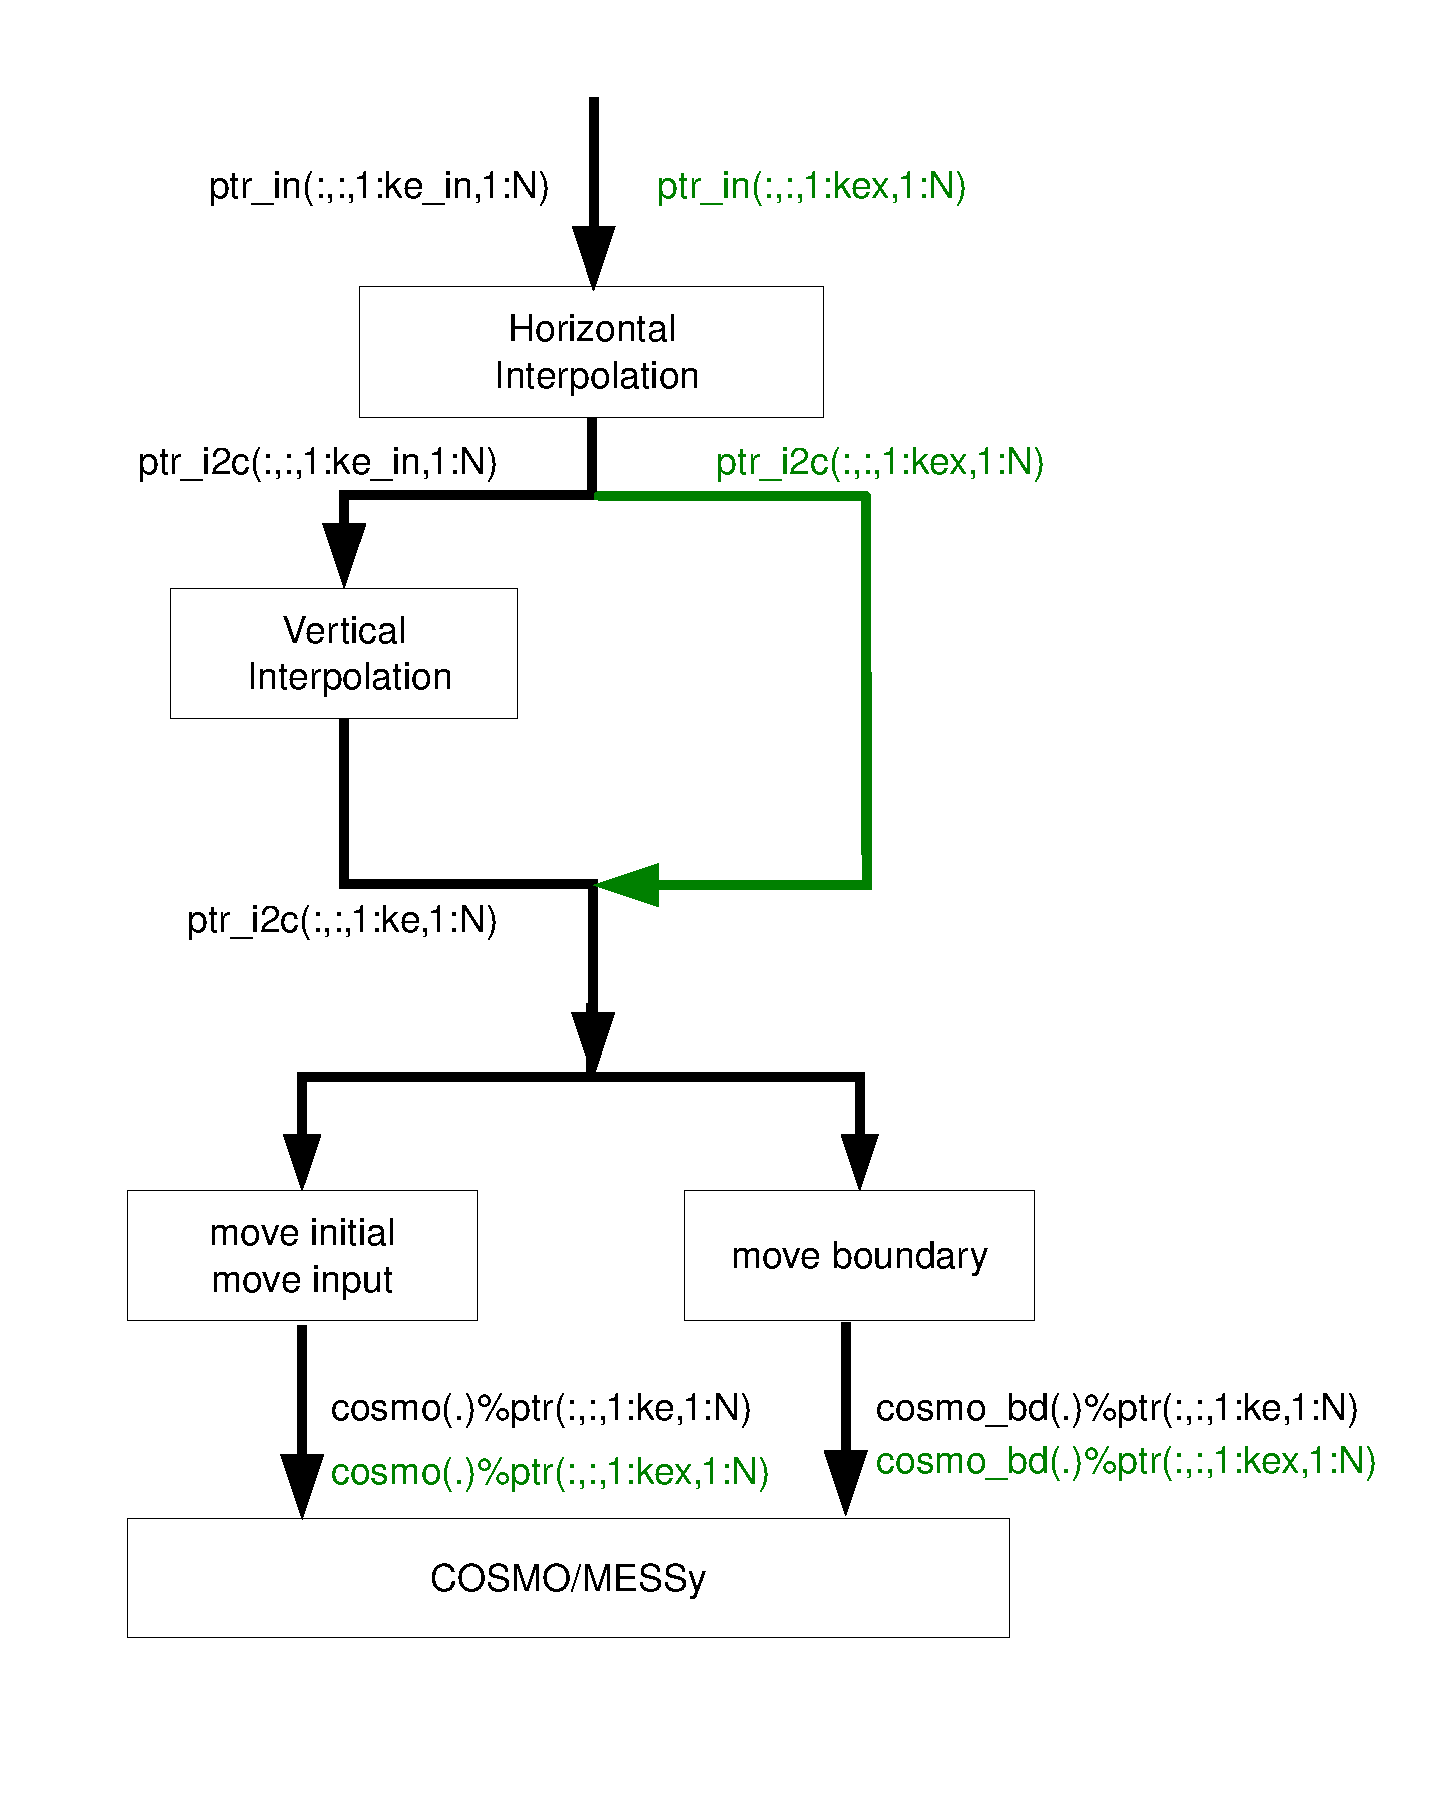
\includegraphics[width=0.99\columnwidth]{MMDUM_ptr.pdf} 
\end{center} 
\vspace*{-.5cm}
\caption{Pointer usage in MMD2WAY\_CHILD. {\tt N} is an arbitrary (number) dimension, 
{\tt ke\_in}
is the number of vertical levels of the {\it in-field}, {\tt ke} is the
number of vertical levels in the COSMO model and {\tt kex} is an arbitrary number
of vertical levels. First, the {\it in-field} is interpolated horizontally,
second, -if requested and possible- the vertical interpolation (black) is 
performed  and third, the {\it intermediate field} is copied to the COSMO/MESSy
target and boundary variables.}
\label{fig:pointer} 
\end{figure} 
%*****************************************************************************
Furthermore, it illustrates the usage of the MMD2WAY\_CHILD internal {\footnotesize POINTER}s:
\verb|ptr_in| is the \textit{in-field}, which is input to INT2COSMO.
During the horizontal interpolation the vertical and number dimensions remain
untouched. The result of the interpolation is written to the \textit{intermediate
field} \verb|ptr_i2c|.  
If the \textit{in-field} is 3D in space (number of incoming
vertical levels is \verb|ke_in|) vertical interpolation is possible. After the
vertical interpolation \verb|ptr_i2c| contains valid data on the vertical levels
\verb|1:ke| with \verb|ke| being the number of vertical levels in the child.
 After the interpolation, the \textit{intermediate field} (\verb|ptr_i2c|) is
copied to the \textit{target field(s)}, i.e., those variables used subsequently
 in the basemodel or other MESSy submodels.
 For \textit{initial} and \textit{input fields} the data is copied to the
 variable
associated with the \verb|cosmo(.)%ptr|, for \textit{boundary fields} the
\textit{intermediate field} is copied to the
boundary variable associated with the {\footnotesize POINTER}s \verb|cosmo_bd(.)%ptr|.


\subsubsection{Finalisation Phase}
After the integration phase at the end of a simulation, the memory allocated in
the course of the simulation is deallocated. The MMD2WAY\_CHILD subroutine 
\verb|mmd2way_child_free_memory| releases the memory allocated by INT2COSMO by
calling 
 the INT2COSMO subroutine \verb|org_cleanup|. For the MMD \verb|test_array| and
 the other memory allocated by MMD the MMD library routines 
\verb|MMD_testC_FreeMem| and \verb|MMD_C_FreeMem| release the memory, 
respectively.

\subsubsection{Grid definitions and parallel decomposition of INT2COSMO}\label{sec:INT2COSMO}
In this section the definition of the different grids and domains used in 
INT2COSMO and the parallel domain 
decomposition of INT2COSMO, which differs from the
INT2LM decomposition, are illustrated.

%%%%%%%%%%%%%%%%
\begin{figure*}
\begin{center} 
%\vspace{-1.3cm}
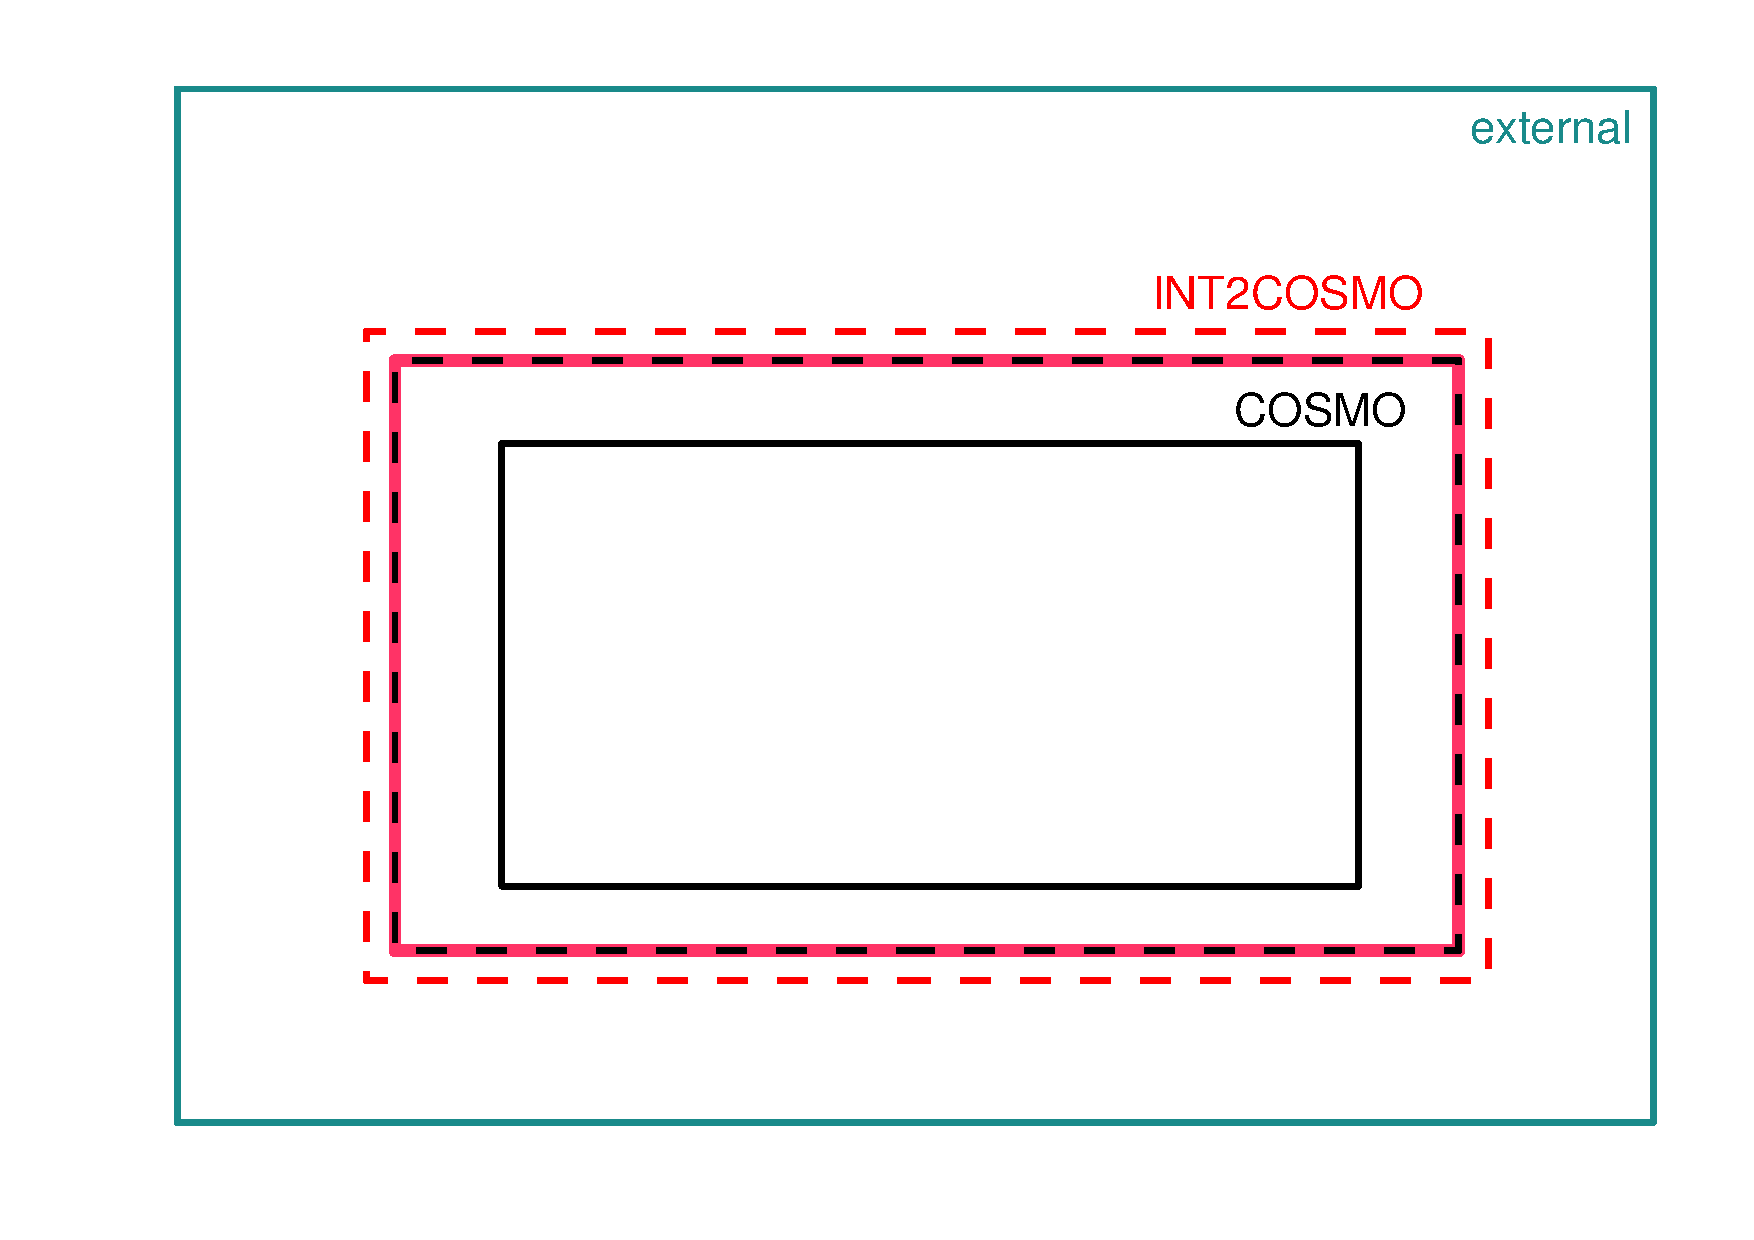
\includegraphics[width=0.6\textwidth]{MMDUM_ext_i2c_c_grids.pdf} 
\end{center} 
\vspace{-.8cm}
\caption{Illustration of the three model domains for the external parameters 
(turquoise), INT2COSMO (red) and the COSMO model (black). The dashed lines 
illustrate the entire model domains, whereas the solid lines show the
 ``inner'' domains (see text).} 
\label{fig:domains} 
\end{figure*} 
%%%%%%%%%%%%%%%%
%%%%%%%%%%%%%%%%
\begin{figure*}
\begin{center} 
\vspace{-1.3cm}
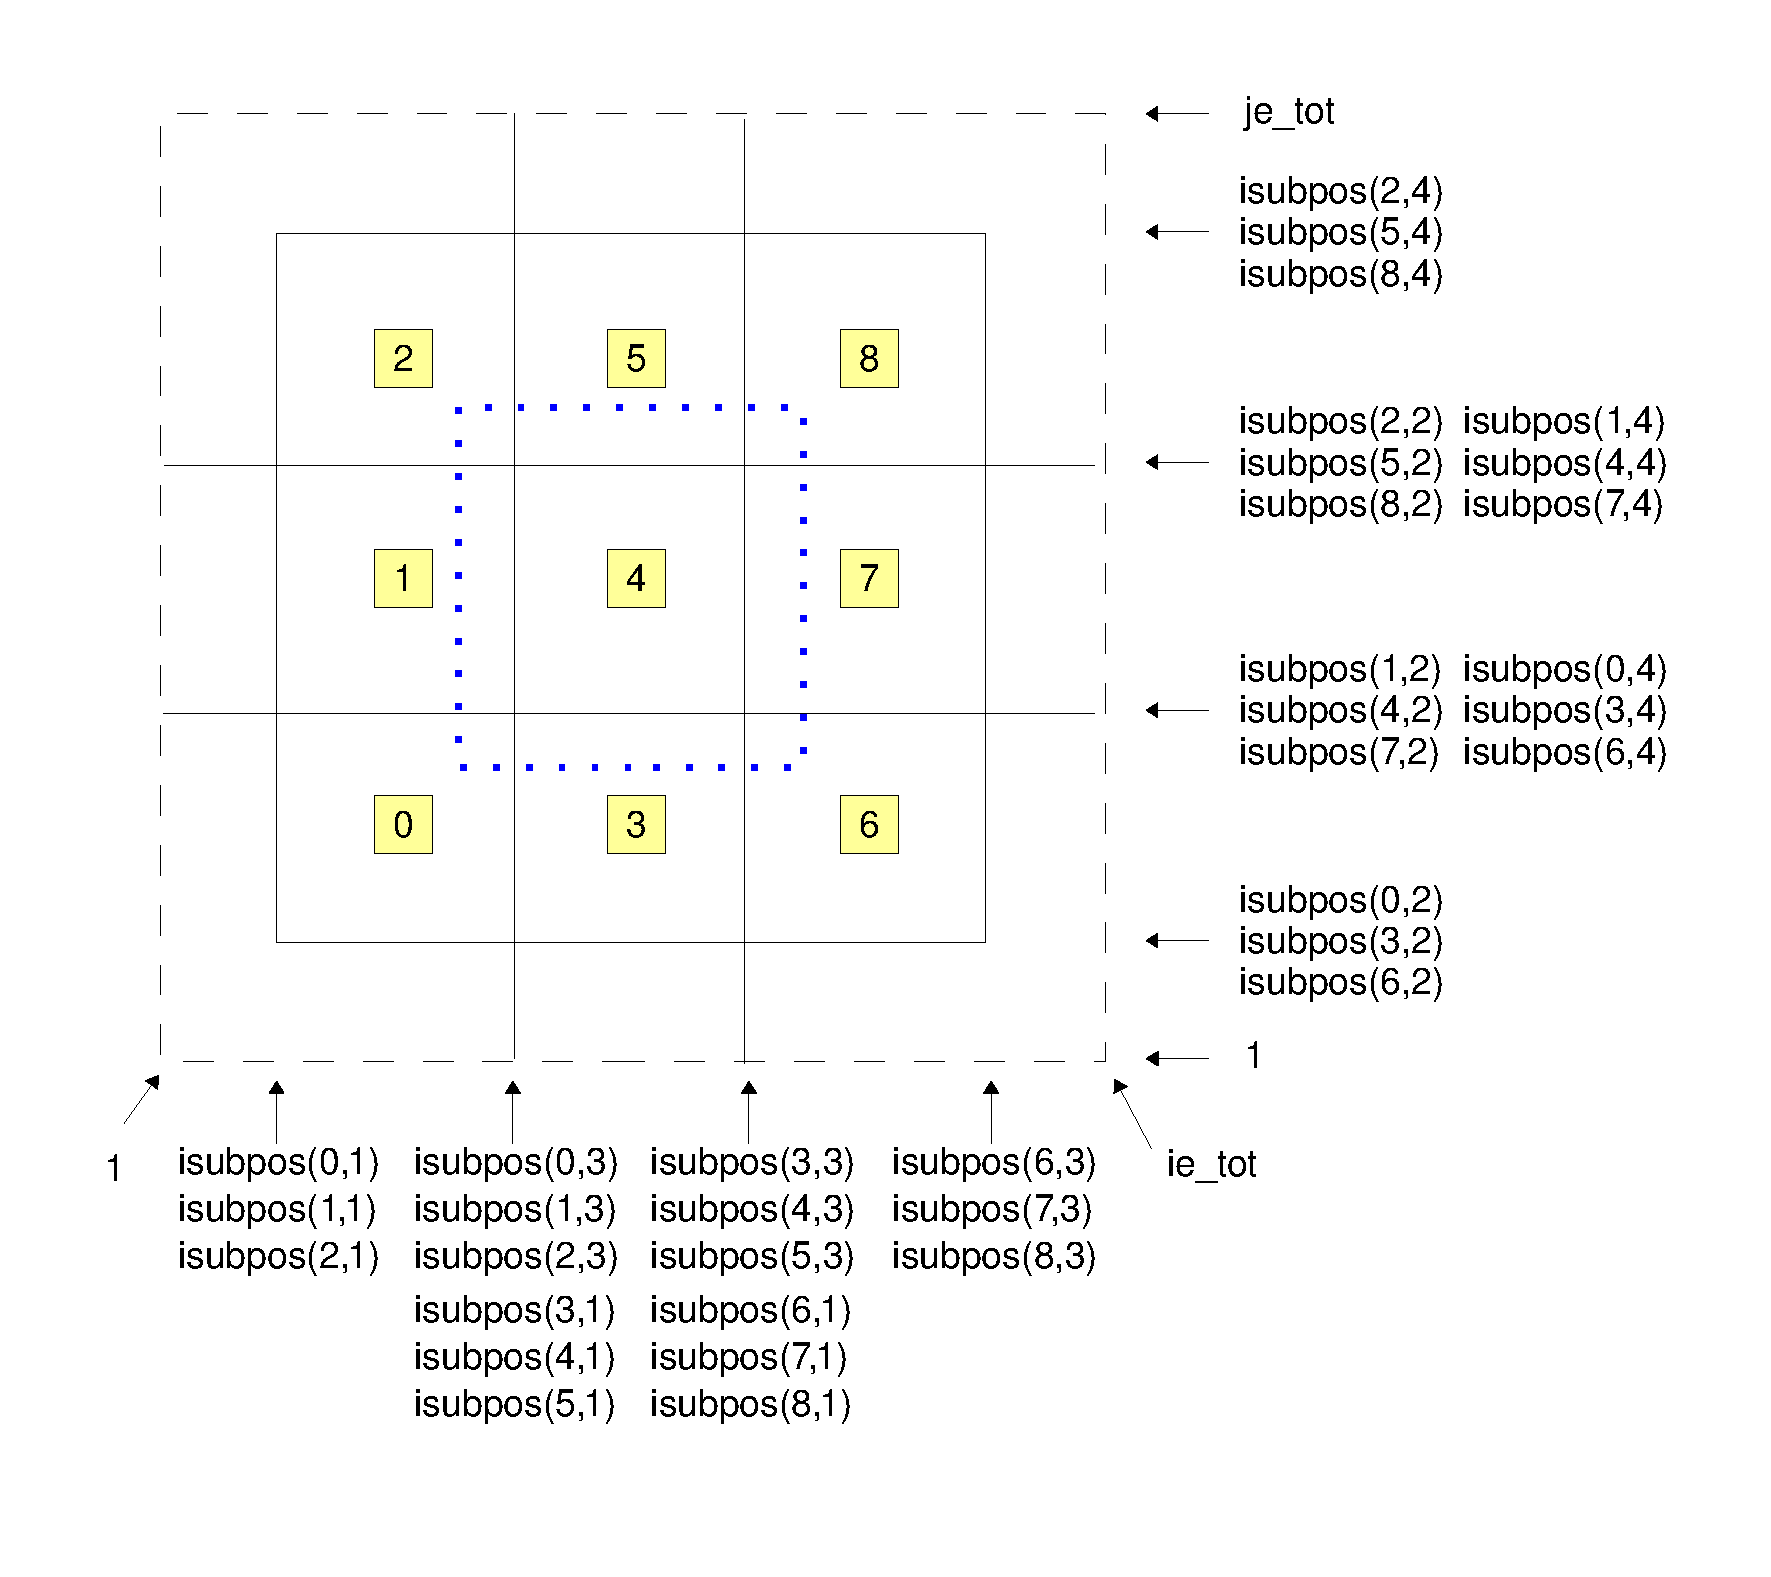
\includegraphics[width=0.9\textwidth]{MMDUM_halo_a.pdf} 
\end{center} 
\vspace{-.8cm}
\caption{Example for a parallel decomposed COSMO model domain, distributed on
3x3 PEs: The numbers on yellow background are the respective PE 
numbers. The black dashed line is the border of the entire model domain, 
the solid lines depict the core-regions of the local domains. The blue dotted 
line indicates the full local domain of PE 4, i.e., including the halo or
ghost boundaries. Additionally annotated are the global indices for
of the core-regions.} 
\label{fig:decomp_globidx} 
\end{figure*} 
%%%%%%%%%%%%%%%%
%%%%%%%%%%%%%%%%
\begin{figure*}
\begin{center} 
%\vspace{-1.3cm}
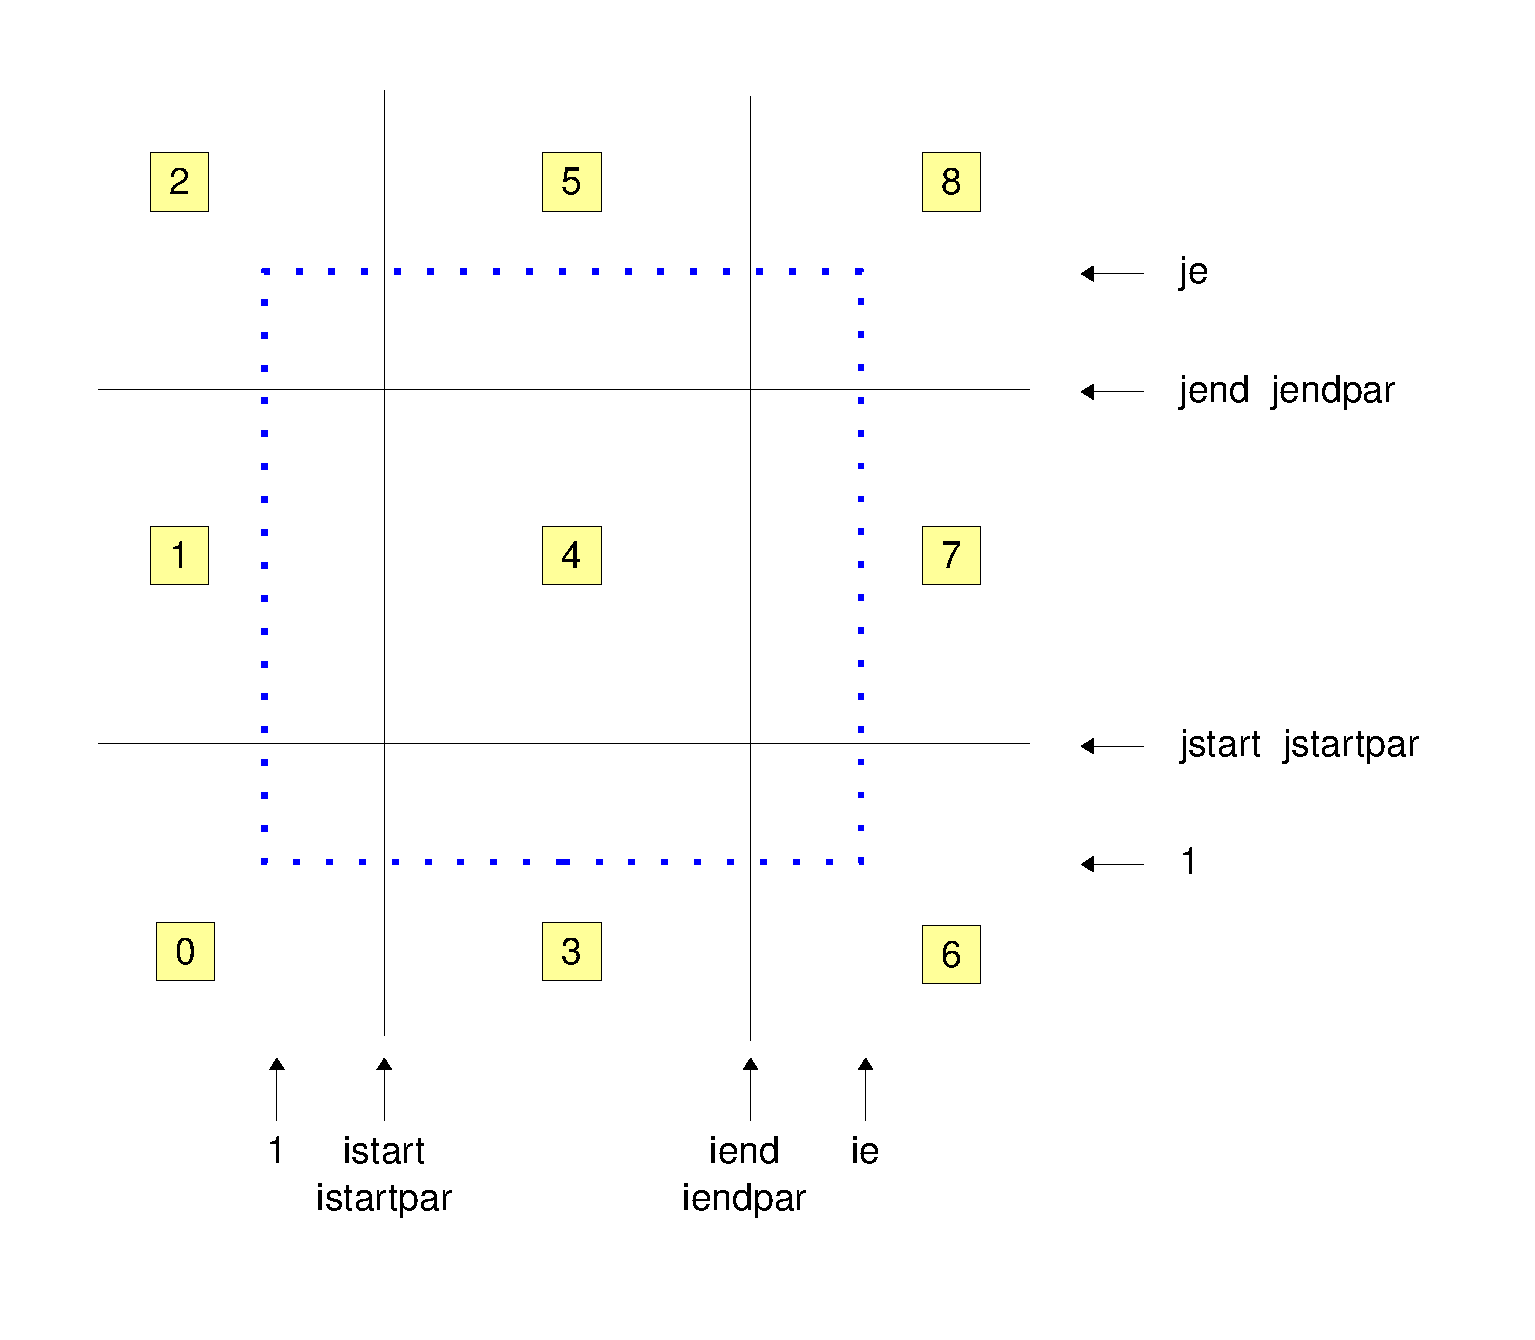
\includegraphics[width=0.45\textwidth]{MMDUM_halo_b.pdf} 
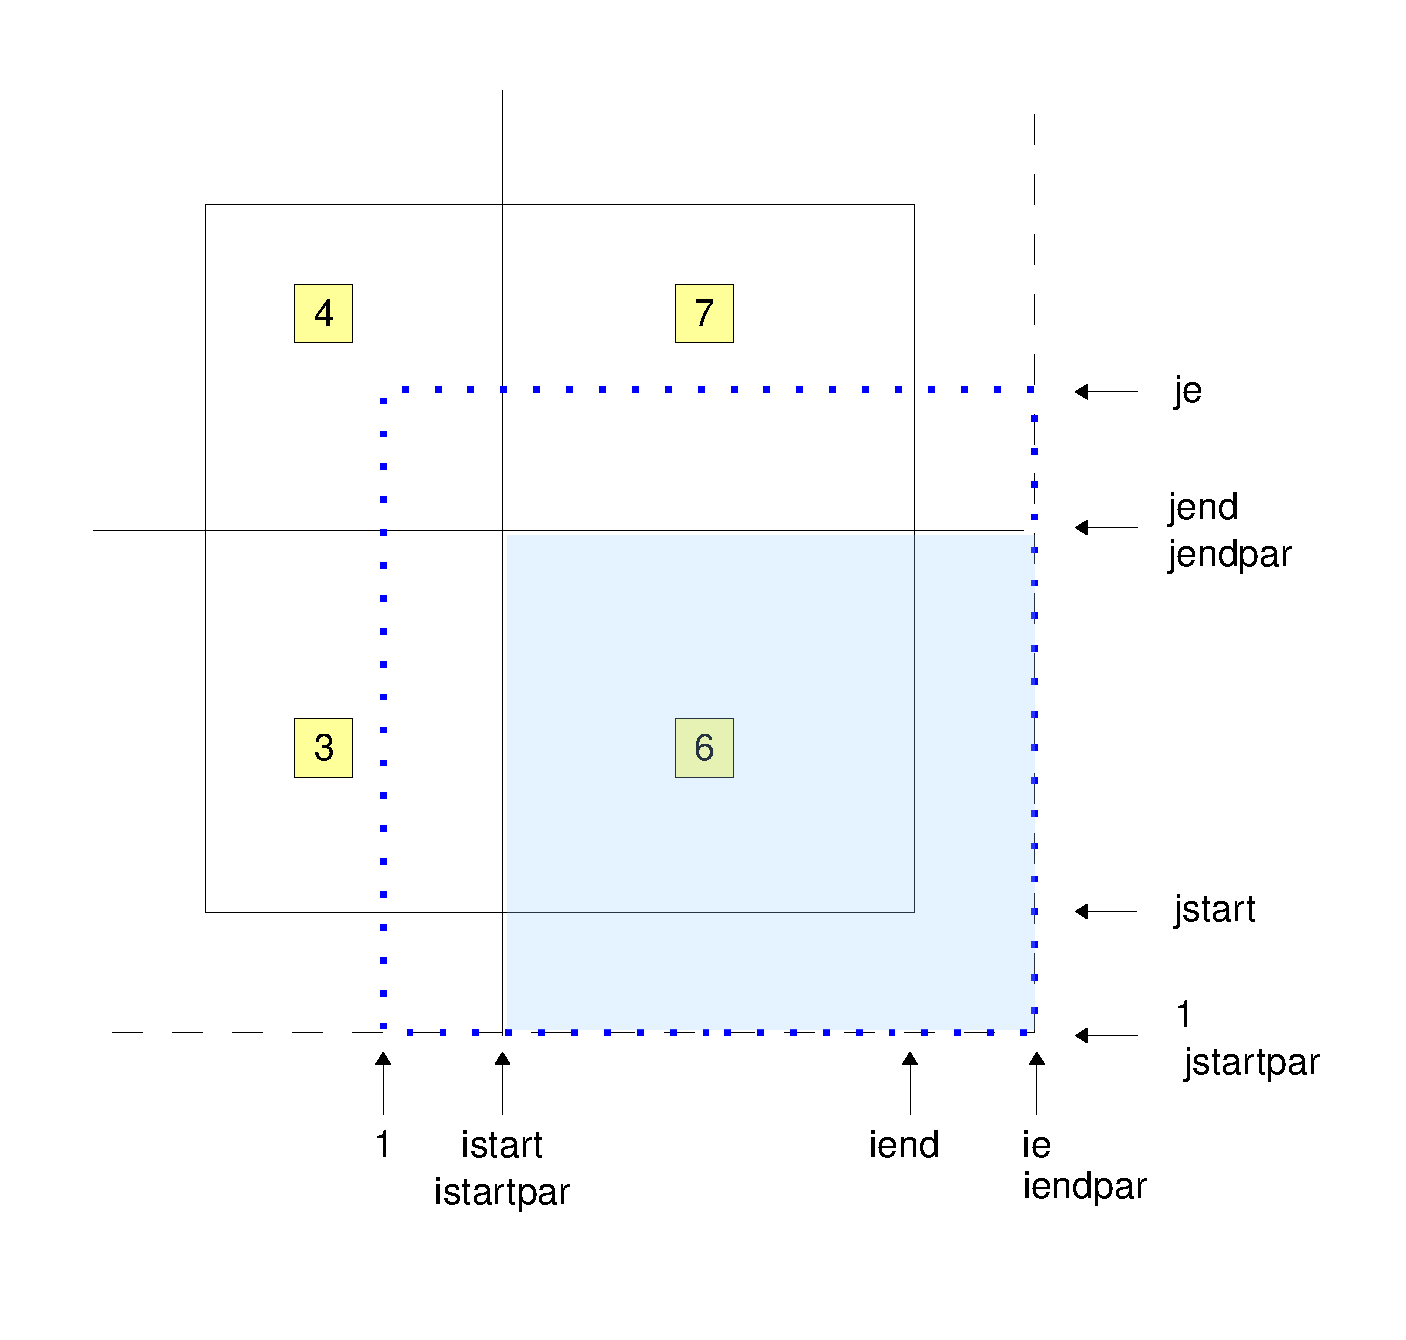
\includegraphics[width=0.45\textwidth]{MMDUM_halo_c.pdf} 
\end{center} 
\vspace{-.8cm}
\caption{The figure is zooming in on PE 4 (left) and PE 6 (right) of Fig.\ 
\ref{fig:decomp_globidx}, illustrating the definition of the local indices
{\tt istart}, {\tt iend}, {\tt jstart}, {\tt jend}, {\tt istartpar}, 
{\tt iendpar}, {\tt jstartpar} and {\tt jendpar}.}
\label{fig:decomp_locidx} 
\end{figure*} 
%%%%%%%%%%%%%%%%
\paragraph{Domains\\}
INT2COSMO works with data defined on four different domains:
\begin{itemize}
\item[1.] The domain of the fields provided by the parent model, i.e., the
{\it in-grid} or the {\it in-field} domain;
\item[2.] the target domain, i.e., the COSMO model domain;
\item[3.] the INT2COSMO domain, i.e., the ``working'' domain of INT2COSMO;
\item[4.] the domain on which the external parameters such as root depth, the 
orography, the leaf area index or the land-sea mask, are defined. 
\end{itemize}
Table \ref{tab:domain1} lists which structure components of the MMD2WAY\_CHILD
variable 
CplData are defined on which domain.
\begin{table} 
\begin{center}
\caption{List of CplData structure components and their respective model domain. \label{tab:domain1}}
{\blockcode
\begin{tabular}{l|l}
structure component & domain \\\hline
{\tt CplData(ii)\%ptr\_in} & {\it in-field} domain \\
{\tt CplData(ii)\%ptr\_i2c}& INT2COSMO domain \\
{\tt CplData(ii)\%cosmo(:)\%ptr} & COSMO domain \\
{\tt CplData(ii)\%cosmo\_bd(:)\%ptr} & COSMO domain \\\hline
 \end{tabular}
}
\end{center}
\end{table}

The {\it in-field} domain is defined by the parent (see Sect.\ 
\ref{sec:Sinitcpl}) and therefore independent of the target COSMO model domain.

The other three domains, must have the same grid spacing and need to be 
rotated in the same way. In other words, the only difference between these model
 domains is their size. The size of the domains is obvious:\\

external parameter domain $>$ INT2COSMO domain $ >$ COSMO domain\\

This hierarchy is caused by the processing order:
\begin{itemize}
\item INT2COSMO processes external parameters. Consequently, the external
parameter fields need to be larger than the INT2COSMO fields.
\item INT2COSMO interpolates data to the COSMO domain, thus the INT2COSMO domain
has to be larger than the COSMO domain.
\end{itemize}
The model domains are illustrated in Fig.\ \ref{fig:domains}.

\paragraph{The parallel decomposition of the COSMO model grid and the 
INT2LM grid\\}
INT2LM and the COSMO model use the same decomposition procedure.
The domain is split into rectangular parts according to the numbers of PEs in
x and y directions (\verb|nprocx| and \verb|nprocy| as namelist entries). 
Figure \ref{fig:decomp_globidx} shows a decomposition for 9 PEs (3x3). 
The parts enclosed by the solid lines illustrate the so-called  ``core-regions''
of the local  (i.e.,\ PE-bound) model domains. The sum of the core-regions covers 
the entire model domain, except for a frame at the lateral boundaries, which 
relevance becomes clear below (i.e., entire domain = ``inner'' domain + lateral
frame).

These core-regions are unambiguously defined by their indices in the 
entire model domain. The indices are stored
in the {\footnotesize INTEGER ARRAY} variable \verb|isubpos(0:nPE-1,4)|, 
with \verb|nPE| number of PEs. 
This variable lists the indices of the lower left and the 
upper right corner of the core-regions of each PE in the entire model domain:
\begin{itemize}
\item \verb|isubpos(:,1)|: first (\verb|'i'|) index  of the lower left corner; 
\item \verb|isubpos(:,2)|: second (\verb|'j'|) index of the lower left corner; 
\item \verb|isubpos(:,3)|: first (\verb|'i'|) index of the upper right corner; 
\item \verb|isubpos(:,4)|: second (\verb|'j'|) index of the upper right corner.
\end{itemize}
Figure \ref{fig:decomp_globidx} illustrates the definition of the individual
\verb|isubpos| for the example. 

To allow the computationally efficient  implementation of  processes, 
which require the data of the neighbour grid points, a ``halo'' or
 ``ghost boundaries'' are defined surrounding the core-region of each PE.
Thus, the local decomposed domain on each PE consists of the ghost boundaries
 and the core-region\footnote{Note: The width of the ghost boundaries and
of the lateral frame are identical. It is defined by the namelist variable 
{\tt nboundlines}.}.
The blue dotted line in Fig.\ \ref{fig:decomp_locidx} illustrates the 
local model domains of PE 4 (left) and PE 6 (right), including the ghost 
boundaries and the core-region.
Physical processes are calculated on the core-region,
whereas the ghost boundaries are used, if the neighbouring value is required
during the calculation of a process, e.g., for advection.
Before calculating such a process, it must be ensured, that the ghost boundaries
contain the correct values for the required fields.
This is achieved by the subroutine \verb|exchg_boundaries|, which transfers the
data from the PE, on which a grid point belongs to the core-region, to the
ghost boundary of the neighbouring PEs.

Figure \ref{fig:decomp_locidx} illustrates the definitions of the local grid and
the respective indices for example PEs 4 and 6:
\begin{itemize}
\item The lower left corner of the local domain is always the grid point 
\verb|(1,1)| and the upper right 
corner is \verb|(ie,je)| with \verb|ie| and \verb|je| being the number of 
grid points in x or y direction, respectively. 
\item The lower left corner of the core-region is \verb|(istart,jstart)|
 and the upper right corner is \verb|(iend,jend)|.
\end{itemize}
 If the PE is not completely surrounded by other PEs, the PE also hosts 
a part of the lateral frame of the entire model domain. In this case, the 
physical processes need also to be calculated on the lateral frame. The lateral
frame is not a part of a core-region, but it is identical to the ghost boundaries
of the respective PE. Thus, the physical processes are also calculated on the
ghost boundaries which is visualised by the right hand side of Fig.\ 
\ref{fig:decomp_locidx}. PE 6 is located at the lower right corner of the
entire model domain. Thus, to calculate the processes on the entire model 
domain, on the eastern and southern border the physical processes are also 
calculated on the ghost boundaries.
While \verb|istart, jstart, iend| and \verb|jend| always refer to the 
core-region, the indices \verb|istartpar, jstartpar, iendpar| and \verb|jendpar|
 refer to the
grid points on which the physical processes are really calculated. On a
PE completely surrounded by other PEs, these index quadruples are equal, as 
illustrated by the left hand side of Fig.\ \ref{fig:decomp_locidx}. 
The right hand side of  Fig.\ \ref{fig:decomp_locidx} shows the indices as 
defined for a PE at the lateral boundary. 
The solid black rectangle illustrates the core-region, the blue dotted line
the entire local model domain. The light blue area indicates the
domain part, on which the physical processes are calculated for PE 6. 


The width of the ghost boundaries, i.e., the number of grid points (variable
\verb|nboundlines|) added at each side to the core-region, depends on the 
processes taken into account in the simulation.
For the COSMO model using the leap-frog time integration scheme  
\verb|nboundlines|=2 is sufficient. If the Runge-Kutta time integration scheme
is used, \verb|nboundlines| is 3 or 4 depending on the order of the Runge-Kutta 
scheme.
In contrast to this, \verb|nboundlines| for the INT2COSMO domain is  
determined by the order of the interpolation routines. For the currently 
implemented interpolation algorithms  \verb|nboundlines| is always 1.

\paragraph{The parallel decomposition of the INT2COSMO grid\\}
%%%%%%%%%%%%%%%%
\begin{figure*}
\begin{center} 
%\vspace{-1.3cm}
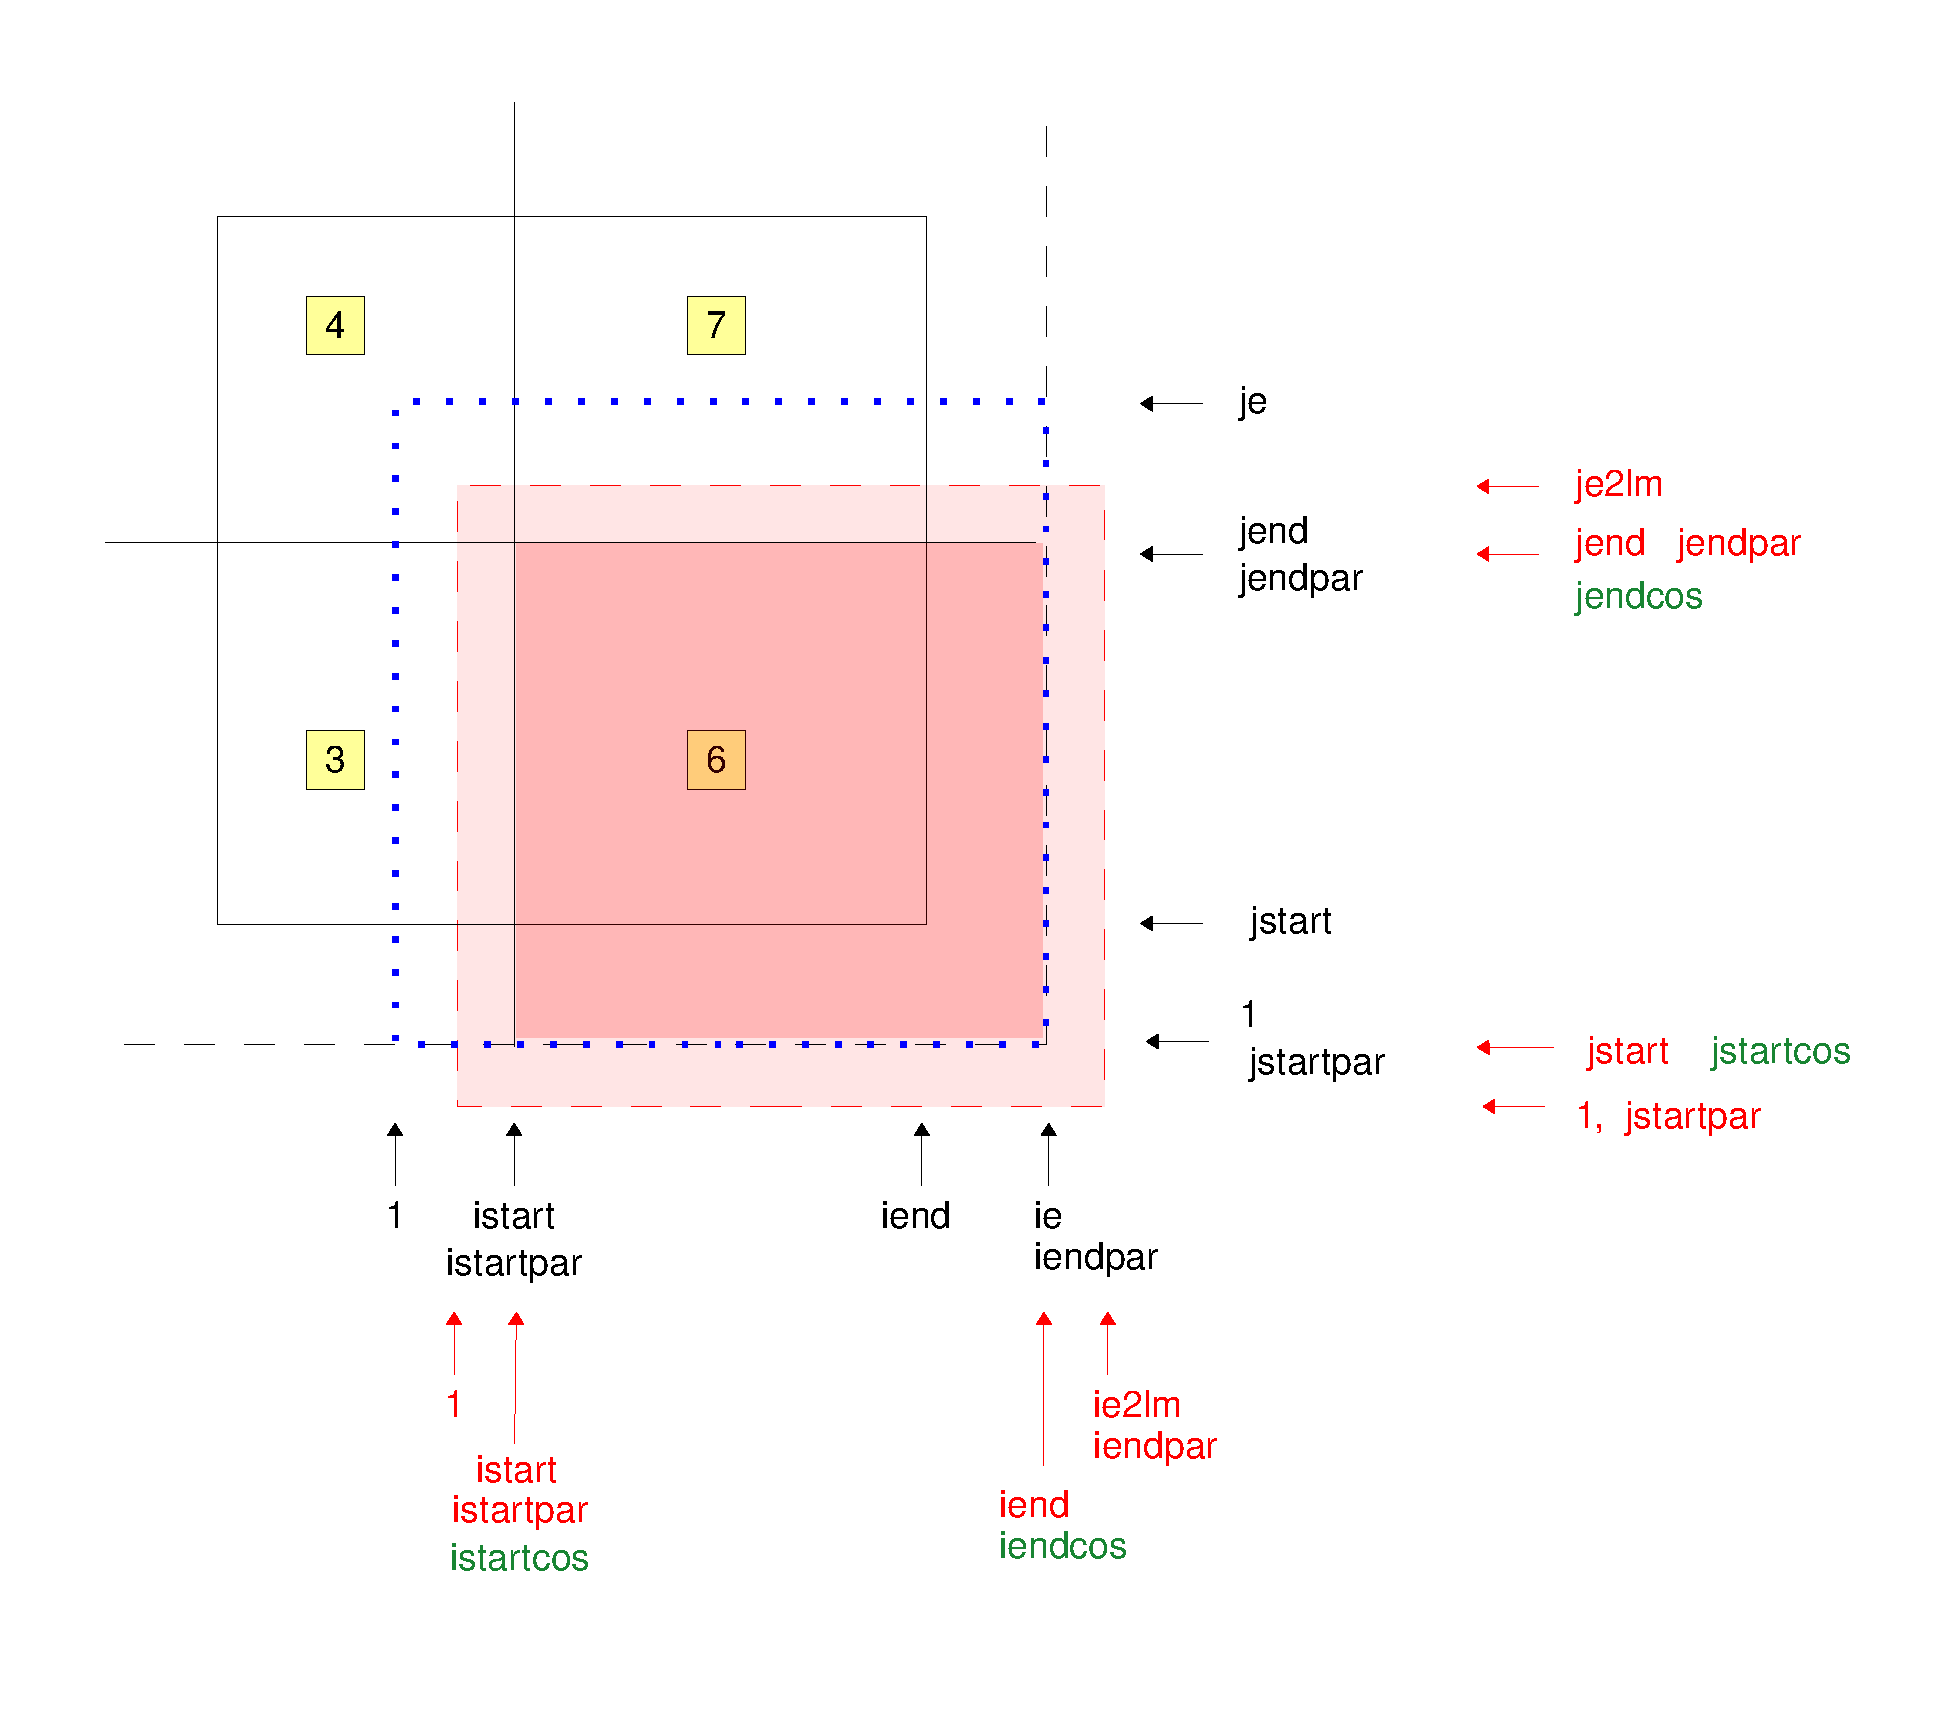
\includegraphics[width=0.75\textwidth]{MMDUM_ixxxcos.pdf} 
\end{center} 
\vspace{-.8cm}
\caption{This is an extension of the right hand side of Fig.\ 
\ref{fig:decomp_locidx}.
Additionally the overlapping INT2COSMO regions for PE 6 are indicated by
red rectangles. The lighter red shows the ghost latitudes, 
whereas the darker red indicates the INT2COSMO core-region. The red indices
are the indices for the local INT2COSMO domain. Additionally, the position
of the four indices  {\tt istartcos}, {\tt iendcos}, {\tt jstartcos} and 
{\tt jendcos} are marked (green colour).}
\label{fig:ixxxcos} 
\end{figure*} 
%%%%%%%%%%%%%%%%

For the sake of computational efficiency, the local INT2COSMO and the local
COSMO model domains should be congruent.
If this is not the case, it is required to gather the fields calculated by
 INT2COSMO on one PE and to scatter them to the local COSMO model
 domains, afterwards.

Unfortunately, the decomposition algorithm used for COSMO and INT2LM does not
lead to a congruent decomposition of both domains, because in
 the decomposition algorithm
\begin{enumerate}
\item an \verb|nboundlines|-wide frame is subtracted from the entire domain, 
\item the remaining domain (called ``inner'' domain) is almost equally 
distributed on the PEs, which leads to the definition of the core-regions, and 
\item the \verb|nboundlines|-wide ghost-boundaries are added to the core-regions
 to define the entire local model domains.
\end{enumerate}
The INT2COSMO domain is larger than the COSMO model domain, and the 
number of ghost boundaries is larger for the COSMO model than for INT2COSMO, 
therefore ``inner'' domains have always different sizes. This is why the
decomposition algorithm cannot result in congruent domains for COSMO and
INT2COSMO.

Nevertheless, it is possible, that the COSMO core-regions are always covered by
the INT2COSMO core-regions.  The coverage of the COSMO core-regions is 
sufficient to avoid the gather and scatter procedure for the complete fields. 
Nevertheless, it requires additional data exchange, for the ghost boundaries.
 This is performed by the COSMO subroutine \verb|exchg_boundaries|.
The coverage of the COSMO core-regions by the INT2COSMO core-regions
can be achieved by skilfully defining the
INT2COSMO core-regions based on the COSMO core-region definition.
The procedure is outlined below:
The INT2COSMO domain is larger than the COSMO model domain, i.e., the 
entire COSMO model domain is equal to the ``inner'' INT2COSMO
domain, i.e., the entire domain minus an \verb|nboundlines| wide frame
(compare Fig.\ \ref{fig:domains}).
Therefore, the INT2COSMO core-regions can be made equal to the
COSMO core-regions for all PEs, except for those at the lateral boundaries. Here
the INT2COSMO core-regions are larger than the COSMO core-regions. 
To be more precise, (following the calculation outlined below) the INT2COSMO 
core-regions at the lateral boundaries are equal to the parts of the local
COSMO model domain described by the indices 
\verb|istartpar|, \verb|jstartpar|, \verb|iendpar| and \verb|jendpar|.

Coverage can only be achieved, if the core-regions of the decomposed COSMO 
model are taken as base for the calculation of the decomposed INT2COSMO grid.
Thus, the \verb|isubpos| definition of the COSMO model domain (further on
denoted as \verb|isubpos_cosmo|) is taken and the INT2COSMO variable 
\verb|isubpos| is calculated from this variable.
For the PEs not located at the lateral boundaries of the model domain 
\verb|isubpos| of the INT2COSMO domain is equal to 
\verb|isubpos_cosmo+nboundlines|, with \verb|nboundlines=1| for INT2COSMO.
\verb|nboundlines| must be added, as the global indices are shifted by 
\verb|nboundlines| in the INT2COSMO grid.

In addition to this shift by \verb|nboundlines|, at the lateral boundaries it has
 to be taken into account, that the ``inner''
 INT2COSMO domain equals the entire COSMO model domain. Thus, as the 
\verb|isubpos_cosmo| are the indices of the ``inner'' COSMO domain, these need
to be shifted by \verb|nboundlines_cosmo| in order to equal the indices of the
 entire model domain.
Thus \verb|isubpos| for PEs at the lateral boundaries of the INT2COSMO domain is 
calculated by:
\begin{eqnarray*}
{\tt isubpos(.,1)} = {\tt isubpos}_{\rm COSMO} - {\tt nboundlines}_{\rm COSMO} + 1 
\end{eqnarray*} 
at a western lateral boundary,
\begin{eqnarray*}
{\tt isubpos(.,2)} = {\tt isubpos}_{\rm COSMO} - {\tt nboundlines}_{\rm COSMO} + 1 
\end{eqnarray*} 
for a southern lateral boundary,
\begin{eqnarray*}
 {\tt isubpos(.,3)} = {\tt isubpos_{\rm COSMO}} +  {\tt nboundlines}_{\rm COSMO} +1
\end{eqnarray*} 
at a eastern lateral boundary and
\begin{eqnarray*}
 {\tt isubpos(.,4)} = {\tt isubpos}_{\rm COSMO} +  {\tt nboundlines}_{\rm COSMO} +1
\end{eqnarray*} 
at a northern lateral boundary.

Because of this procedure, the core-regions of the INT2COSMO domain and those
of the COSMO model domain are not equal at the lateral boundaries.
In order to copy the data from the fields defined on the INT2COSMO domains
correctly to the fields defined on the COSMO model domains, additional indices
are required to indicate the co-location of the COSMO local domains
 on which the physical processes are calculated (i.e., those indicated by
\verb|istartpar, jstartpar, iendpar| and \verb|jendpar|) and the INT2COSMO 
core-regions. The indices \verb|istartcos|, \verb|iendcos|, 
\verb|jstartcos| and \verb|jendcos| are defined in a similar manner as 
\verb|istartpar, jstartpar, iendpar| and \verb|jendpar| by:

\begin{eqnarray*}
\tt istartcos &=& 1 + \tt  nboundlines\\
\tt iendcos &=& \tt ie2lm - \tt  nboundlines\\
\tt jstartcos &=& 1 + \tt  nboundlines\\
\tt jendcos &=&  \tt  je2lm - \tt nboundlines\\
\end{eqnarray*} 
with \verb|ie2lm| and \verb|je2lm| being the dimension of the local INT2COSMO
domains (similar to \verb|ie| and \verb|je| for the decomposed COSMO domain).
This is illustrated by Fig.\ \ref{fig:ixxxcos}.

%+++++++++++++++++++++++++++++++++++++++++++++++++++++++++++++++++++++++++++
%+++++++++++++++++++++++++++++++++++++++++++++++++++++++++++++++++++++++++++
%+++++++++++++++++++++++++++++++++++++++++++++++++++++++++++++++++++++++++++


\subsection{The parent instance\label{sec:c2pParent}}
For the 1-way coupling, the parent instance fulfills three tasks, which are
essential for the on-line coupling: 
\begin{itemize}
\item It dictates the date/time and {\it restart} settings of the child model.
\item It calculates the \verb|index_list|, i.e., the association of the child
and the parent instance grid points on the individual PEs.
\item It provides the {\it exchange fields}.
\end{itemize}

Comparably to MMD2WAY\_CHILD, in MMD2WAY\_PARENT the data for the data
exchange is organised in a Fortran95 structure:

\begin{verbatim}
  ! CplData STRUCTURE
  TYPE T_COUPLE_C_DATA
     ! CHANNEL AND CHANNEL OBJECT NAMES IN PARENT MODEL
     TYPE(t_chaobj_cpl)                    :: name
     ! POINTER TO PARENT FIELD
     REAL(DP), POINTER, DIMENSION(:,:,:,:) :: ptr => NULL()
     ! REPRESENTATION OF PARENT FIELD
     INTEGER                               :: rank
     INTEGER, DIMENSION(4)                 :: ldimlen=0
     ! STRING ORDER OF AXES
     CHARACTER(LEN=4)                      :: AXIS
  END TYPE T_COUPLE_C_DATA
\end{verbatim}
As for the 1-way coupling the parent instance only provides data, the Fortran95
structure contains considerably less components than the corresponding
structure of MMD2WAY\_CHILD.
Whereas a child can have one parent, a parent can have more than one
child.
 Therefore, the variable of {\footnotesize TYPE} \verb|T_COUPLE_C_DATA| 
 (\verb|CplData|) is itself component of a structure 
({\footnotesize TYPE}~\verb| T_CHILD_DATA|).

\begin{verbatim}
  TYPE T_CHILD_DATA
     ! NUMBER OF EXCHANGED FIELDS
     INTEGER                                       :: NEXCH
     TYPE (T_COUPLE_C_DATA), DIMENSION(:), POINTER :: CplData => NULL()
     ! POINTER for DATA EXCHANGE TIMING
     REAL(DP), POINTER                             :: Waittime => NULL()
     ! LOGICAL for COUPLING TIME STEP (evaluated in init_loop, required in
     !  init_loop and global start)
     LOGICAL                               :: lcpl = .FALSE.
  END TYPE T_CHILD_DATA

  TYPE (T_CHILD_DATA), DIMENSION(:), ALLOCATABLE :: CL
\end{verbatim}
The Fortran95 variable \verb|CL| is allocated to the number of child
instances of the respective parent instances in the initialisation phase.

\subsubsection{Initialisation Phase}\label{sec:c2pParentInit}
In the initialisation phase three MESSy entry points are used by
MMD2WAY\_PARENT:
\verb|mmd2way_parent_initialize|, \verb|mmd2way_parent_init_memory| and
\verb|mmd2way_parent_init_coupling|.
\paragraph{\bf mmd2way\_parent\_initialise\\}
The parent inquires the number of child instances it has to provide data 
for. The MMD library variable \verb|MMD_Parent_for_Child| is a list of the
 parent specific child instance IDs in the MMD setup. In each parent it is
 allocated to the specific number of child instances the respective
 parent instance has to deal
 with. Thus the {\footnotesize SIZE} of this array equals the number of 
children  of the parent.
Subsequently, the MMD library initialisation routines 
\verb|MMD_P_Allocate_Child| and 
\verb|MMD_P_Init| are called to initialise the MMD environment of this 
specific parent instance. \verb|MMD_P_Allocate_Child| accepts a
parameter \verb|l2way|: it is \verb|.FALSE.| for 1-way coupling
and \verb|.TRUE.| for 2-way coupling.

In MMD2WAY\_PARENT itself, the variable \verb|CL| is dimensioned
to the number of children. As each child may require a different coupling 
frequency, the TIMER {\it event} variables \verb|CPL_EVENT| and 
\verb|CPL_IOEVENT| must also be available for each child instance individually.

\paragraph{\bf mmd2way\_parent\_init\_memory\\}\label{sec:Sinitmem}
First, independently for each child the time synchronisation of the
respective child-parent pair is triggered by calling \verb|Setup_Child_Timer|:
\begin{enumerate} %%e1+
\item The parent receives the coupling interval in seconds from the 
child and defines the respective TIMER {\footnotesize EVENT} 
(\verb|CPL_EVENT(ic)|).
\item Next, the parent sends its date information and its time step
length to the child.\\
The following dates must be exchanged to ensure that the models are
synchronised: 
\verb|current_date|, \verb|start_date|, \verb|resume_date| and \verb|stop_date|.
The dates are of {\footnotesize TYPE} \verb|time_days|:
\begin{verbatim}
  TYPE, PUBLIC :: time_days 
     !
     ! relative calendar date and time format
     !
     ! time_days [structure]
     !   day    [integer]  (day in calendar, -2147483648 ..... 2147483647
     !                      approx. +/-5.8 Mio. years)
     !   second [integer]  (seconds of day, 0,...,86399)
     !
     !PRIVATE
     LOGICAL :: init   = .FALSE.
     INTEGER :: day    = 0
     INTEGER :: second = 0
  END TYPE time_days
\end{verbatim}
Thus, each date is defined by an {\footnotesize INTEGER} indicating the day and
 an {\footnotesize INTEGER} for the seconds of the day. For all four dates these
 two {\footnotesize INTEGERs} are packed into an {\footnotesize INTEGER} array
 and 
sent to the child. As a ninth {\footnotesize INTEGER} the time step 
length of the parent is sent. The latter is used by the child to define
 the \verb|BREAK_EVENT|. 
\end{enumerate}%%e1-

\paragraph{\bf mmd2way\_parent\_init\_coupling\\}\label{sec:Sinitcpl}
The preparations for the 1-way coupling are all performed in the subroutine
\verb|mmd2way_parent_init_coupling|. 
The subroutines described below are processed for each child model
individually (indicated below by the index \verb|ic|).

\begin{itemize} %1+

\item First, the MMD library subroutine
\verb|MMD_P_Get_DataArray_Name| is called, which receives the list of {\it 
exchange fields}. After calling this subroutine, these information is
available within the MMD 
library, but not yet made available to MMD2WAY\_PARENT itself. 
This transfer is done within the subroutine \verb|Define_data_arrays| 
(see last item below).

\item
Before the {\it exchange fields} themselves are acquired,
the domain section required by the child model for the interpolation of the
data,  
i.e., the domain of the {\it in-fields} of the child model are determined in the
subroutine \verb|Setup_Child_Area|.
\begin{itemize} %%i2+
\item In a first step the parent model acquires the child model grid information:
\begin{itemize} %%i3+
\item First, the parent gets the 
dimensions of the child model COSMO domain (\verb|ie_tot| and \verb|je_tot|)
 and the 
 number of {\it exchange fields}.
\item Second, according to the dimensions, fields are allocated for the 
geographical longitudes and latitudes of the COSMO/MESSy grid points,
\item which are, third, sent subsequently from the child to the parent.
\end{itemize} %%i3-

\item Based on the child grid, the domain of the data sent to the child
is determined:
\begin{itemize} %%i3+
\item If a COSMO/MESSy model is the parent, the complete COSMO/MESSy
parent domain is used as {\it in-field} for the child model. In this
case simply the information about the parent model COSMO grid are copied to the
respective transfer variables: i.e., \verb|startlat_tot|, \verb|startlon_tot|, 
\verb|endlat_tot|, \verb|endlon_tot|, \verb|pollat|, \verb|pollon|, \verb|dlat|
, \verb|dlon|, \verb|ie_coarse|, \verb|je_coarse|, \verb|ke_coarse|
, \verb|ke_soil_coarse|, \verb|itype_w_so_rel|, \verb|itype_t_cl|, 
\verb|vcoord%vcflat|, \verb|svc1|, \verb|svc2|, \verb|vcoord%ivctype|
and the derived type \verb|refatm|, with its components defining the reference
atmosphere \verb|refatm%p0sl|, \verb|refatm%t0sl|, \verb|refatm%st0lp|, 
\verb|refatm%delta_t| and \verb|refatm%hscal|,  
 and the depth of the soil layers (\verb|czmls|).

\item If ECHAM5/MESSy
 is the parent instance, a subset of the global grid is provided as input to 
INT2COSMO. The size of the domain is determined by the minimum and maximum
longitudes and latitudes of the child model domain, including a check whether
the 
date line is part of the model domain. As INT2COSMO requires a somewhat larger 
model domain as the COSMO grid to perform the interpolation, four grid boxes are
added at each side of the model domain\footnote{The size of 4 is arbitrarily
chosen, because it worked for the standard ECHAM5/MESSy
 resolutions so far employed. The really required size depends, e.g., on the
 rotation of the child grid}. 
From this model domain, the location of
the corners of the grid in the parallel decomposition of the global model are 
calculated by the subroutine \verb|locate_in_decomp|.

\begin{itemize} %%i4+
 \item The geographical coordinates of the
 South-West corner determine the start latitude (\verb|startlat_tot|) and 
longitude (\verb|startlon_tot|) and
\item those of the North-Eastern corner the end latitude (\verb|endlat_tot|) and 
 longitude (\verb|endlon_tot|).
\item The coordinates of the rotated pole, \verb|pollat| and  \verb|pollon|, are
 always \verb|90._dp| and \verb|180._dp| for a non-rotated grid like the ECHAM5 grid. 
\item The grid spacings in degrees for the
 longitudes of the global grid (\verb|dlon|) is easily 
calculated by dividing \verb|360._dp|  by the {\footnotesize SIZE} of the
variables containing the Gaussian longitudes of the global grid.
\item The latitudes of a Gaussian grid are not equidistant, however, the grid 
spacings in degrees is a mandatory input to INT2LM also for the latitudes. Thus,
the method implemented in INT2LM when reading and checking the netCDF-file 
global definitions (subroutine \verb|read_nc_gdefs|) 
\begin{verbatim}
   dlat = (MAXVAL(philat) - MINVAL(philat))/(ngl-1)
\end{verbatim}
is used.
To minimise the error, \verb|dlat| is recalculated after the determination of the
section of the grid that is sent to the child using the maximum and minimum
latitude of the sent section. Note: as the latitudes in a Gaussian grid are 
not equidistant this only works satisfactorily if the regional model region
is not too close to the poles (with ``to close'' depending on the ECHAM5 
resolution). 

\item The horizontal dimensions of the exchanged domain \verb|ie_tot| and 
\verb|je_tot|
are calculated according to the difference of the corner indices. 
\item \verb|ke_tot|
is simply \verb|nlev|, i.e., the number of ECHAM5 vertical levels. 
\item  \verb|ke_soil| 
is \verb|4| as ECHAM5 includes a soil with 5 layers and 4 is the number of 
interfaces between the soil layers. 
\item The INT2COSMO variable \verb|itype_w_so_rel|, indicating which type of 
soil moisture is input to INT2COSMO, must be set to \verb|2| 
(for both parent models).
\item  The variable defining the type of the climatological temperature 
\verb|itype_t_cl| is set to \verb|1|, if ECHAM5/MESSy is the parent, and to
 \verb|0|, if  COSMO/MESSy is parent. 
\item Additionally, information about the vertical levels of the model domain,
 i.e., the interface hybrid parameters (\verb|vct|) for ECHAM5/MESSy and 
\verb|vcoord| for the COSMO/MESSy model are sent to the child.
\end{itemize}%%i4-
\item  Last but not 
least, two fields containing the longitudes and latitudes for each server domain
grid point are sent to the child.
\end{itemize} %%i3-
\end{itemize} %%i2-

\item The purpose of the
subroutine \verb|Setup_data_exchange_with_Child| \label{page:calindexlist} 
is to calculate the \verb|index_list|,  
i.e., the list which unambiguously associates the grid points
 with the same geographical coordinates located in the local domains of the 
child  {\it in-field} and in the parent local domain to each
other. Each grid 
point is defined by the process number (PE) the grid point is located on, and 
an index pair $(i,j)$ containing the indices of the grid point in the parallel 
decomposed grids.
Along with determining this list the \verb|test_array| for the MMD consistency 
check is filled. Thus, at the beginning of this subroutine the \verb|test_array|
 is allocated by calling the MMD library routine \verb|MMD_testP_Setup|.

For the calculation of the \verb|index_list| the parent needs the
geographic 
coordinates of the grid points of the local (decomposed) fields from the child.
To exchange these, the parent model first receives three {\footnotesize
INTEGERs}:  
the maximum dimensions for the decomposed horizontal child grid 
(\verb|ie_max| and \verb|je_max|) and the number of child PEs. 
According to these dimensions, the parent allocates two three 
dimensional fields to pick up the decomposed longitude and latitude fields sent
 by the child.

For each of the grid points in the horizontal domain a list member containing
six entries is created. One of these sextuples consists of the child PE 
(PE$_c$), the parent PE (PE$_p$) and the index pairs ($i_c$,$j_c$) and 
($i_p$,$j_p$) of the local decomposed child and parent model domains,
respectively,  associating the two points with the
same geographical coordinates in child and parent grid to each other. 
 The index information about the child grid is inherent
in the longitude and latitude arrays. These fields have been gathered in a way,
that the index of the third dimension corresponds to PE$_c$ and the 
indices of the first two dimensions correspond to the indices in the 
horizontal local grid. 
The longitude and latitude given by the fields
sent by the child are processed by the
subroutine \verb|locate_in_decomp|, which 
locates the respective pair of geographical coordinates on the local decomposed
grid of the parent. Output of this subroutine are the PE on which the
grid point is located (PE$_p$) and the indices in the local fields
($i_p$,$j_p$).  Thus, a sextuple 
containing all required information about the related grid points of the child
and parent domain is complete. Such a sextuple is determined for each of the 
child instance {\it in-field} grid points yielding in a field 
($i_p$,$j_p$,$i_c$,$j_c$,PE$_c$,PE$_p$)$_n$, with $n$ number of grid points.
 Additionally, each sextuple is fed into the MMD
 \verb|test_array| by using the MMD library function \verb|MMD_testP_Fill|.
After all grid points have been processed the filling of the MMD 
\verb|test_array| is finalised by calling the MMD library function 
\verb|MMD_testP_FinishFill|.
The entire \verb|index_list| containing all sextuples is forwarded to the 
MMD library and analysed within the MMD library routine 
\verb|MMD_P_Set_Indexlist| establishing the connections between the 
individual parent and child PEs. A more detailed explanation of this 
list is given in the MMD
 library manual, which is part of the same electronic supplement as this manual.


\item 
Last but not least, the { \footnotesize POINTERs} to the {\it exchange fields}
 must be associated during the initialisation phase. This is achieved in
the subroutine \verb|Define_data_arrays|:
\begin{itemize} %%i2+
\item The structure 
\verb|CL(ic)%CplData|, with \verb|ic| being the index for one child
 instance, is allocated to the number of required {\it exchange fields.} 
\item The {\it channel} and {\it channel object} name of each field and the 
child model {\it representation} as listed in the MMD2WAY\_CHILD namelist are
retrieved by  
calling the MMD library function \verb|MMD_P_GetNextArray|.
\begin{itemize} %%i3+
\item If the {\it channel} name is \verb|'test'| the MMD \verb|test_array| is 
requested
and the {\footnotesize POINTER} is associated by calling the MMD library routine
\verb|MMD_testP_GetTestPtr|.

\item In all other cases the {\footnotesize POINTER} is associated by calling 
the CHANNEL 
subroutine \verb|get_channel_object|. If the object does not exist the
simulation is terminated as the required coupling is not possible. 
\end{itemize}%%i3-

\item When the object exists, the {\it representation ID} is inquired by 
calling the CHANNEL subroutine \verb|get_channel_object_info|. 

\item The {\it representation ID} must be known to 
subsequently retrieve the required dimension informations: 
\begin{itemize}%%i3+
\item the {\it axis string},
\item the local dimension lengths,
\item  the global dimension lengths, and 
\item the {\it representation} name. 
\end{itemize}%%i3-
The latter two are required, if the {\it representation} name given in the
 MMD2WAY\_CHILD 
namelist is \verb|'#UNKNOWN'|. In this case the child
needs the additional information plus a possible {\it attribute} which might 
contain heights (in case of multi-layer emission fields) to create the correct 
{\it representation}. 
This additional {\it attribute} is accessed by the CHANNEL subroutine
\verb|get_attribute|. All these information are forwarded to the child
 by the MMD library function \verb|MMD_P_Send_Repr|.

At the end of the subroutine, the {\footnotesize POINTER}, the {\it axis
string} and the local 
{\it dimensions} are  passed on to the MMD library by the subroutine 
\verb|MMD_P_Set_DataArray| and 
processed inside the library, i.e., the dimensions and the order information
are saved for later use. 

\item After all data fields are processed a last call during the initialisation 
phase
 to the MMD library (subroutine \verb|MMD_P_SetInd_and_AllocMem|)
invokes the final evaluation of the dimension information in order to determine
the correct buffer size. Subsequently, the actual allocation of the buffer
required by MPI takes place calling \verb|MPI_ALLOC_MEM| in the MMD library.
\end{itemize}%%i2-
\end{itemize}%%i1-

\subsubsection{Integration Phase}
During the integration phase, in the
 subroutine \verb|mmd2way_parent_global_start|, 
 the parent provides the {\it exchange fields} to its
child instances. 
Additionally, in the subroutine \verb|mmd2way_parent_global_end| it informs 
the child models,
 whether the simulation is going to be interrupted.

\paragraph{\bf mmd2way\_parent\_global\_start\\}
First, the {\it coupling event} is tested for each child. If the 
coupling with the respective child is scheduled for the current time step,
 the MPI Buffer is filled by calling the MMD library subroutine 
\verb|MMD_P_FillBuffer|. 
Within this MMD library routine the data is copied to the memory buffer
accessible for the child model. To ensure the correct order of accesses to 
the buffer from the parent and the child, the buffer is locked for that
 model of a child-parent pair, which latest wrote to/read the buffer.
 If the workload of the models is not ideally balanced it happens that one of 
the models has to wait until it can access the buffer again.
\verb|MMD_P_FillBuffer| returns the waiting time in seconds for the parent
model.

\paragraph{\bf mmd2way\_parent\_global\_end\\}
At the end of the time loop, the parent sends the information about
the status of the interrupt-switches \verb|lbreak|, \verb|l_rerun|
and \verb|lstop|. If the {\footnotesize LOGICALs} are \verb|.TRUE.|, the 
respective entry of the {\footnotesize INTEGER ARRAY} \verb|timeflags| is set
to  \verb|1|. Otherwise it is set to zero.

\subsubsection{Finalisation Phase}
At the end of the simulation the allocated memory is released.
The subroutine \verb|mmd2way_parent_free_memory| calls, independently for each
child, the MMD library subroutines \verb|MMD_testP_FreeMem| and 
\verb|MMD_P_FreeMem| to release the memory allocated within the library.
Additionally, the MMD2WAY\_PARENT internal
variables \verb|CL(ic)%CplData|, \verb|CL|,  
\verb|CPL_IOEVENT| and \verb|CPL_EVENT| are deallocated.


%+++++++++++++++++++++++++++++++++++++++++++++++++++++++++++++++++++++++++++
%+++++++++++++++++++++++++++++++++++++++++++++++++++++++++++++++++++++++++++
%+++++++++++++++++++++++++++++++++++++++++++++++++++++++++++++++++++++++++++
\section{Coupling of the parent instance to child (2-way,
parent-to-child coupling) \label{sec:p2c}}
%+++++++++++++++++++++++++++++++++++++++++++++++++++++++++++++++++++++++++++
%+++++++++++++++++++++++++++++++++++++++++++++++++++++++++++++++++++++++++++
%+++++++++++++++++++++++++++++++++++++++++++++++++++++++++++++++++++++++++++
The backward coupling from the child to the parent is organized in a
similar way  
as the 1-way coupling, i.e., which input is required from which child
for a specific child is determined in the parent namelists
(Sect.\ \ref{sec:cplparchild}).   

{\footnotesize POINTER}s to the respective memory are acquired in the
child instance and are 
interpolated to the parent instance similar ``{\it out-grid}'' in the
child. 
Subsequently, the interpolated fields are sent to the parent and applied
to the field according to a method determined by the namelist setting
independently for each {\it coupled field}.

In the following, the backward coupling specific routines are described, first
for the parent and second for the child instance.

\subsection{The parent instance}

Four different data types are defined in MMD2WAY\_PARENT in order to organise
the coupling of the parent to the child.

Two of them are required for the reading and processing of the  namelist input
of the \verb|&CPL_PAR_CHILD| namelist:
\begin{verbatim}
  TYPE T_EXCH_P_IO
     ! CHANNEL AND CHANNEL OBJECT NAMES IN PARENT  
     TYPE(t_chaobj_cpl)                    :: Parentname
     TYPE(t_chaobj_cpl)                    :: Parenttend
     TYPE(t_chaobj_cpl)                    :: Childname
     ! Representation String
     CHARACTER(LEN=STRLEN_MEDIUM)          :: REPR = ''  ! REPRESENTATION STRING
     ! FLAG FOR INTERPOLATION METHOD
     INTEGER                               :: interp = 0 ! INTERPOLATION METHOD
     ! FLAG FOR APPLICATION METHOD overwrite (input field) in GridPoint (appl=0)
     ! FLAG FOR APPLICATION METHOD weighted in GridPoint (1)
     INTEGER                               :: appl = 0   ! application method
     !  weighing factor for "nudging" 1 = hard nudging
     REAL(dp)                              :: fac = 1._dp
  END TYPE T_EXCH_P_IO

  ! MAXIMAL NUMBER OF EXCHANGE FIELDS
  INTEGER, PARAMETER                        :: NMAX_P_EXCH = 100
  TYPE(T_EXCH_P_IO), DIMENSION(NMAX_P_EXCH) :: PFIELD
  TYPE(T_EXCH_P_IO), DIMENSION(NMAX_P_EXCH) :: DEFAULT_PFIELD

  TYPE T_P_EXCHG_DATA_IO
     ! use generalised humidity couplings
     LOGICAL                                   :: lgrhum      = .FALSE.
     INTEGER                                   :: i_rmy_px    = 0
     REAL(dp)                                  :: pcontrol_fi = 30000.
     INTEGER                                   :: itype_fw    = 2 
     INTEGER                                   :: icosexp     = 14
     REAL(dp)                                  :: damprel     = 0.2_dp
     INTEGER                                   :: itype_VI    = 1 
     INTEGER                                   :: RCF         = 10000
     INTEGER                                   :: RCF_in      = 10000
     LOGICAL                                   :: ldiagonly = .FALSE.
     TYPE(T_EXCH_P_IO), DIMENSION(NMAX_P_EXCH) :: FIELD
     ! allow for free boundary layer
     LOGICAL                                   :: lfreeslip   = .FALSE.
     LOGICAL                                   :: lcpl_gs     = .FALSE.
  END TYPE T_P_EXCHG_DATA_IO

  TYPE(T_P_EXCHG_DATA_IO), DIMENSION(:), ALLOCATABLE :: PIO
\end{verbatim} 
Here, \verb|PIO| of TYPE \verb|t_p_exchg_data_io| contains all possible
contents of a \verb|CPL_PAR_CHILD| namelist, while \verb|PFIELD| of
TYPE \verb|t_exch_p_io| is required to read the array of {\it exchange fields}
 (see Sect.\ \ref{sec:cplparchild}).
The 1D array variable \verb|PAR| is of the derived type \verb|T_COUPLE_P| 
 and contains all information required for the
coupling of all child instances of a specific parent.
 It is allocated to the number of coupled child instances early during the 
initialiation. This structure contains the 1D array variable \verb|CplData|,
 which is of type \verb|T_COUPLE_P_DATA|, providing all data required for the 
coupling of the individual field. This is allocated to the actual number of 
{\it exchange fields} for the respective child at the end of the
namelist interpretation (see Sect.\ \ref{sec:interpretparnamelist}).
\begin{verbatim}
  ! PARENT CplData STRUCT
  TYPE T_COUPLE_P_DATA
     ! CHANNEL AND CHANNEL OBJECT NAMES IN PARENT  
     TYPE(t_chaobj_cpl)                    :: Parentname
     TYPE(t_chaobj_cpl)                    :: Parenttend
     TYPE(t_chaobj_cpl)                    :: Childname
     ! POINTER TO FIELD in Parent model which will be changed
     ! (i.e. for prognostic variables the tendency !)
     REAL(DP), POINTER, DIMENSION(:,:,:,:) :: target => NULL()
     ! POINTER TO FIELD in Parent model required for tendency calulation
     ! (i.e. the m1 field for prog. vars, otherwise  nothing  !)
     REAL(DP), POINTER, DIMENSION(:,:,:,:) :: targetm1 => NULL()

     ! POINTER TO FIELD yielding the interpolated Child fields
     REAL(DP), POINTER, DIMENSION(:,:,:,:) :: ptr => NULL()
     ! TRACER INDEX
     INTEGER                               :: idt = -99
     ! REPRESENTATION OF PARENT FIELD
     INTEGER                               :: rank
     ! coupling to tendency
     LOGICAL                               :: lte = .FALSE.
     INTEGER, DIMENSION(4)                 :: ldimlen=0
     INTEGER, DIMENSION(4)                 :: gdimlen=0
     ! STRING ORDER OF AXES
     CHARACTER(LEN=4)                      :: AXIS
     ! FLAG FOR INTERPOLATION METHOD 
     ! 1 conservative
     ! 2 bilinear ... (to be implemented)
     INTEGER                               :: interp = 0
     ! FLAG FOR APPLICATION METHOD 
     !  0: as 1: only possible for input fields (i.e., channel objects made by
     !           'mmd2way_parent' itself, not for tendency calculation, not for
     !           tracer (for the parent, the source can of course be a
     !           tracer!) 
     !          for appl = 0 the input field is simply transformed to the
     !          full 2D/ 3D parent grid (where frac >0.9999) without 
     !          application of any weight function 
     !          flagged (i.e., they are /= 0 only where the weigth function is 1
     !  1: field exists only in GridPoint (1) => change tendency
     !     will be worked on in global start
     INTEGER                               :: appl = 0
     !  weighing factor for "nudging" 1 = hard nudging
     REAL(dp)                              :: fac = 1._dp
     ! Representation String
     CHARACTER(LEN=STRLEN_MEDIUM)          :: REPR
     ! is time dependent ? (relevant Only for COSMO parent)
     LOGICAL                               :: ltimedep
     ! mmd parent has to define its own memory                     
     LOGICAL                               :: l_SentUnit = .FALSE.
  END TYPE T_COUPLE_P_DATA

  TYPE T_COUPLE_P
     ! NUMBER OF EXCHANGE FIELDS 
     INTEGER                                       :: NEXCH
     TYPE (T_COUPLE_P_DATA), DIMENSION(:), POINTER :: CplData => NULL()
     ! POINTER for DATA EXCHANGE TIMING
     REAL(DP), POINTER                             :: Waittime => NULL()
     ! Lon /Lat of incoming data
     REAL(kind=dp),      DIMENSION(:,:,:), POINTER :: all_plon => NULL()
     REAL(kind=dp),      DIMENSION(:,:,:), POINTER :: all_plat => NULL()

     ! weight fractions summed over all child PEs
     REAL(dp),             DIMENSION(:,:), POINTER :: frac => NULL()
     REAL(dp),             DIMENSION(:,:), POINTER :: mask => NULL()
     INTEGER                                       :: kmin    
     REAL(dp), DIMENSION(:), POINTER               :: kminfac => NULL()

     ! weighting function
     REAL(dp),             DIMENSION(:,:), POINTER :: wf => NULL()

     ! ENTRIES FOR GENERALIZED HUMIDITY COUPLING:
     ! use generalised coupling
     LOGICAL                                       :: lgrhum = .FALSE.
     ! data index for vapor
     INTEGER                                       :: idx_qv = -99
     ! data index for cloud water
     INTEGER                                       :: idx_qc = -99
     ! data index for cloud ice
     INTEGER                                       :: idx_qi = -99
     ! data index for meridional wind
     INTEGER                                       :: idx_u  = -99
     ! data index for zonal wind
     INTEGER                                       :: idx_v  = -99
     ! data index for deriv. of meridional wind
     INTEGER                                       :: idx_t    = -99
     ! data index for surface pressure
     INTEGER                                       :: idx_ps   = -99
     
     ! NAMELIST SWITCHES

     ! treatment of boundary zone for back transition
     INTEGER                                       :: i_rmy_px  = 0 
     REAL(dp)                                      :: pcontrol_fi = 30000.

     INTEGER                                       :: itype_fw  = 2 
     INTEGER                                       :: icosexp   = 14
     REAL(dp)                                      :: damprel   = 0.2_dp
     INTEGER                                       :: RCF       = 10000
     INTEGER                                       :: RCF_in    = 10000
     LOGICAL                                       :: ldiagonly = .FALSE.
     ! itype_VI switches the vertical interpolation  of C2E
     ! == 1  => NCREGRID
     ! == 2  => INT2LM inverse (MesoTel version)
     INTEGER                                       :: itype_VI  = 1
     !
     ! allow for not forced boundary layer
     LOGICAL                                       :: lfreeslip = .FALSE.
     LOGICAL                                       :: lcpl_gs   = .FALSE.

     REAL(DP), POINTER, DIMENSION(:,:) :: aps => NULL()

  END type T_COUPLE_P

  TYPE(T_COUPLE_P), DIMENSION(:), ALLOCATABLE :: PAR

  ! -----------------------------------------------------------------------
\end{verbatim}

The meaning of the components of the derived type variables has already been
explained in Sect.\ \ref{sec:cplparchild} or will be explained in the following.

\subsubsection{mmd2way\_parent\_initialise}
In addition to the inquiry of the number of child instances and the
initialisation of the MMD library, which both are required for the 1-way
coupling, the variable \verb|PAR| is allocated to the number of child instances 
and the parent namelists in the namelist file \verb|mmd2way.nml|
are read.
As explained in Sect.\ \ref{sec:namelist} the \verb|mmd2way.nml| namelist file
can contain an arbitrary number of  \verb|&CPL_PAR_CHILD| namelists.
These namelists are attributed to one specific child instance by the
entry \verb|INSTANCE|. If the number given by \verb|INSTANCE| is the index of
one of the child instances of the 
parent, this specific namelist is used. However, the first \verb|&CPL_PAR_CHILD|
 namelist in the namelist file \verb|mmd2way.nml| determines the default
 setting, which will be used for all instances, for which no individual
 namelist is provided.

At the end of the subroutine \verb|mmd2way_parent_initialize| the derived
type array PIO, containing all information available from the namelist is
filled completely. 

\subsubsection{mmd2way\_parent\_init\_memory}
In a loop over all child instances of the specific parent,
memory is allocated for fields required for the backward transfer from
 the child instance:
\begin{itemize}
\item The {\it channel object} \verb|'weightfrac'| is a horizontal field
containing for each grid cell the fraction overlapping with the area sent 
by the child model.
\item The {\it channel object} \verb|'weightfunc'| is a horizontal field and 
provides the weight 
with which each grid cell will be weighted, when applied to an existing field
of the parent. This weight function depends on the chosen type
 (namelist parameter \verb|itype_fw|) and is calculated by the child
(see page \pageref{descript:itype_fw}).
\item The {\it channel object} \verb|kminfac|, which is a vertical column and
contains the vertical weighting coefficients for the vertical application of
the field. 
\end{itemize}
For each child model, the index of the child model is appended to the {\it
channel object} name, as the names of the {\it channel objects} for one parent
need to be unique.

\subsubsection{mmd2way\_parent\_init\_coupling}
The subroutine \verb|mmd2way_parent_init_coupling| performs the main parts for
the child-parent coupling.
\begin{itemize} %l1+
\item {\bf interpret\_parent\_namelist:\label{sec:interpretparnamelist}\\}
The interpretation of the parent namelist entries works in the same
way as the
interpretation of the namelist of the child for child-to-parent coupling.
The namelist can contain wildcards. In this case, the respective child {\it
channel} 
must contain the same {\it objects} as the parent model {\it channel}.
The namelist parameters are described in detail in
Sect.\ \ref{sec:cplparchild}.
After the analysis of the namelist, the component \verb|CplData| of the
derived type variable \verb|PAR| is allocated to the number of respective
{\it exchange fields} and filled with the contents of the intermediate input /
output variable \verb|PIO|. As this investigation is performed only in the I/O
PE, finally the content of \verb|PAR| is broadcasted to all parent instance PEs.
\item In a loop over the child models the namelist content is sent to the
respective child model. However, while the control parameters are simply
broadcasted, the fields are transfered via the MMD library:
\begin{itemize} %l2+
\item {\bf MMD\_P\_Set\_ParDataArray\_Name:} 
The MMD library is filled with required information about the {\it exchange
fields}. These are: the parent {\it channel} and {\it channel object} name, the
child model {\it 
channel} and {\it channel object} name, the representation, the interpolation
method and a {\footnotesize LOGICAL} determining whether the unit of
the {\it coupled field} should be sent from the child to the parent.
\item The namelist input determining the size and the weights of the area
coupled back to the parent, plus some additional information are sent to the
respective child model using \verb|MMD_Inter_Bcast|. The respective namelist
switches
are: \verb|lgrhum|, \verb|i_rmy_px|, \verb|pcontrol_fi|, \verb|itype_fw|, 
\verb|icosexp|, \verb|damprel|, \verb|RCF|, \verb|RCF_IN|, \verb|itype_VI|
and \verb|ldiagonly|. 
\end{itemize}%l2-
\item In a second loop over the child instances (loop index \verb|ic|),
\begin{enumerate} %l2+
\item  the parameter 
\verb|rdheight|, indicating the height in which the damping at the model top
starts, is received from the respective child model 
via the MMD library subroutine \verb|MMD_Recv_from Child|.
As the damping zone is not coupled back to the parent model, the parent model
subsequently calculates the vertical index of the layer of its own model
domain, in which \verb|rdheight| is
located and above which the coupling coefficients are zero.
This index (\verb|PAR(ic)%kmin|) is sent to the child model and used later on 
in both models to define {\it channel objects} of reduced height for the {\it
exchange fields}. 
\item the subroutines \verb|MMD_P_Get_DataArray_Name|
and \verb|Setup_Child_Area| are called. They are both required for the 1-way
coupling.
\item the subroutine \verb|Setup_ParData_Exchange| is called. In this
subroutine the \verb|index_list| for the parent-to-child coupling is calculated.
The procedure is the same as for the child-to-parent coupling as
described in Sect.\ \ref{sec:c2pParentInit}
(more specific
page \pageref{page:calindexlist}). The \verb|index_list| is sent to the child 
via \verb|MMD_Send_to_Child|. The exchange information required by the
parent are finally acquired by calling the MMD library
subroutine \verb|MMD_P_Get_ParIndexList|. In addition to the direct grid
association information, two additional fields are received:
\begin{itemize} %l3+
\item the fractional overlap of the child model grid with
the respective parent grid box (\verb|PAR(ic)%frac|), and 
\item the weight function
(\verb|PAR(ic)%wf|) containing the weights that should be assigned to the
respective parent grid box calculated by the child.
\end{itemize} %l3-
At the end of the subroutine, a mask for the fields that are influenced by
more than 99,999\% is calculated allowing for simpler postprocessing of data
only defined in the coupling region.

\item At the end of this loop over the child instances the
subroutines \verb|Setup_Data_Exchange_with_Child|
and \verb|Define_data_arrays| are called. Both have been explained in the
context of the 1-way coupling.
\end{enumerate} %i2-
\item In a third loop over the childrn (loop index \verb|ic|),
the memory is set up for the exchange of the {\it exchange
fields}. Additionally, the vertical nudging coefficient is calculated.
\begin{enumerate}%i2+
\item The newly calculated index \verb|PAR(ic)%kmin| is used to define
two new {\it representations} for the {\it coupling fields} with reduced height,
i.e., the 3D {\it representations} \verb|'GP_3D_RDCX'|
and \verb|'GP_3D_RDCXp1'| for mid point and interface fields are defined.
\item The nudging factor for the vertical \verb|Par(ic)%kminfac| is
calculated. In all vertical levels
below \verb|Par(ic)%kmin| it is preset with \verb|1._dp|. 
From \verb|Par(ic)%kmin| on to the model top it is
preset with \verb|0._dp|. At the moment a quarter cosine function is
prescribed, which is
zero at level \verb|Par(ic)%kmin| and reaches \verb|1._dp| 10 levels below.\\
For experimental purposes a similar function can be used at the surface by
setting the namelist switch \verb|lfreeslip = .TRUE.|. But this cosine
function spreads over 3 levels only.

\item Finally, the memory required for the {\it exchange fields} is allocated
in a loop over the {\it coupling fields}, established by calling the MMD library
function \verb|MMD_P_GetNextParArray|. Different cases are accounted for:
\begin{itemize}%i3+
\item A prognostic variable should be changed by the coupling by influencing
its  tendency:\\
\begin{itemize}%l4+
\item For later use the {\footnotesize LOGICAL }switch \verb|Par(ic)%CplData(ii)%lte| is set 
\verb|.TRUE.| indicating that the tendency will be changed.
\item The {\footnotesize POINTER} to the tendency field (\verb|Par(ic)%CPLData(ii)%target|)
 is associated to the respective parent
 model field by calling the subroutine \verb|get_channel_object|.
\item The {\footnotesize POINTER} to the prognostic field at the end of the last time step
 (\verb|Par(ic)%CPLData(ii)%targetm1|) 
 is associated to the respective parent
 model field by calling the subroutine \verb|get_channel_object|.
\item In a next step, the information, if the prognostic field includes a
 dimension for time levels (as is the case for many COSMO model variables),
 is generated. If such a dimension exists the {\footnotesize LOGICAL }switch 
\verb|Par(ic)%CPLData(ii)%ltimedep| is set to \verb|.TRUE.|.
\end{itemize} %l4-

\item A prognostic variable should be changed by changing the prognostic field
itself:\\
\begin{itemize}%l4+
\item The {\footnotesize POINTER} to the prognostic field (\verb|Par(ic)%CPLData(ii)%target|)
 is associated to the respective parent
 model field by calling the subroutine \verb|get_channel_object|.
\item The {\footnotesize POINTER}  (\verb|Par(ic)%CPLData(ii)%targetm1|) is NULLYfied in this 
case. Note: the {\footnotesize POINTER} \verb|Par(ic)%CPLData(ii)%target| always points to the 
object which should be changed.
 
\item In a next step, the information if the prognostic field includes a
 dimension for time levels (as is the case for many COSMO model variables)
 is generated. If such a dimension exists the {\footnotesize LOGICAL }switch 
\verb|Par(ic)%CPLData(ii)%ltimedep| is set to \verb|.TRUE.|.
\end{itemize} %l4-
\item The field is only diagnostic input to the parent and the parent
 has to allocate the memory for this field itself:\\
\begin{itemize}%l4+
\item In this case a new {\it channel object} is created by
calling the subroutine \verb|new_channel_object|. Additionally, if the
knowledge of the unit was requested 
(\verb|Par(ic)%CPLData(ii)%l_SentUnit ==.TRUE.|), the unit is acquired from
the child model by calling \verb|MMD_Inter_Bcast|. Subsequently, the received
unit is defined as a {\it channel object attribute}.
\end{itemize} %l4-
\end{itemize}%l3-
Independent of the {\it target field}, memory for the {\it exchange field}
needs to be 
allocated. Dependent on the {\it representation} of the {\it target field},
the {\it representation} of the {\it exchange field} is determined.
Subsequently, the {\footnotesize POINTER} (\verb|Par(ic)%CPLData(ii)%ptr|) is allocated by
calling the subroutine \verb|new_channel_object|. 
\end{enumerate}%l2-

Afterwards, additional
information, as the rank, the axis string and the global and local field
length are acquired by calling \verb|get_representation_info|.
The newly allocated field, and the information about the local dimensions and
the axis string are provided to the MMD library upon calling the MMD library
subroutine \verb|MMD_P_Set_ParDataArray|.

To enable a special treatment of certain prognostic variables (especially for
diagnostics during the development phase) the indices of these variables are
saved.

\end{itemize}%l1-

At the very end of the subroutine \verb|mmd2way_parent_init_coupling| the
MMD library routine \verb|MMD_P_SetInd_and_AllocMem| is called. This is
required for 1-way and 2-way coupling. Internally, in the case of 2-way
coupling the memory of the exchange buffer is allocated to the maximum size
required for the data exchange.

\subsubsection{mmd2way\_parent\_global\_start}
If the coupling to the child is due, the buffer is filled here. The only
difference to the 1-way coupling is, that the \verb|Waittime| is not
investigated here in case of 2-way coupling.

\subsubsection{mmd2way\_parent\_global\_end}
The subroutine \verb|mmd2way_parent_global_end| is called three times,
therefore the subroutine is called with a parameter \verb|flag|. 
The call with \verb|flag=2| invokes the exchange of the TIMER status. This has
already been discussed in \ref{sec:restarttriggers}.

In the calls with \verb|flag=1| or \verb|flag=3| the actual change of the
parent fields takes place. In a loop over the child instances, 
\begin{enumerate}
\item it is
checked, whether this time step is a coupling time step. If so,
for \verb|flag=1| first the buffer exchange takes place by calling the MMD
library routine \verb|MMD_P_GetBuffer|. In the case of actual 2-way coupling
the \verb|Waittime| is provided by \verb|MMD_P_GetBuffer|. The times are
necessarily inquired, after the child model had the access to the exchange
buffer. Thus different
locations for the \verb|Waittime| inquisition are required.
\item  for \verb|flag = 1| or \verb|3| the
subroutine \verb|mmd2way_parent_couple_gp| is called. Depending on the flag
the tendencies (\verb|flag=1|) or the full fields (\verb|flag=3|) are changed.
\end{enumerate}

If ECHAM5 is the parent instance the calls proceed just one after the other (in
the order 1,3,2), while
for a COSMO parent, the subroutine is called from three distinct points
in the time loop:
\verb|flag=1| is called before the subroutine call to  
\verb|organize_dynamics('compute', ...)|, as in this subroutine the
integration of the tendencies proceeds, the tendencies need to be changed
beforehand.
\verb|flag=3| and \verb|flag=2| are called directly before the COSMO model
subroutine call \verb|organize_data('result', ...)|. Note, that the order of
the calls is \verb|flag=3|, \verb|flag=2| as the exchange of the timer
information is performed last.

Within the subroutine \verb|mmd2way_parent_couple_gp| in  a loop over all
{\it exchange fields}, first it is tested whether the current field should be
changed in this call, i.e., tendencies are only changed if 
\verb|flag=1| and \verb|Par(ic)%CPLData(ii)%lte = .TRUE.|, fields are  
only directly changed, if \verb|flag=3| and 
\verb|Par(ic)%CPLData(ii)%lte =.FALSE.|. Otherwise the loop is cycled.

For each field loops over the two horizontal (index \verb|jp, jrow|) and the
vertical 
dimensions (\verb|jk|) are performed. For 3D fields, the vertical loop reaches
from \verb|Par(ic)%kmin| down to the surface. 

For each horizontal grid box it is checked, if the grid box is fully covered
by the 
child domain (\verb|Par(ic)%frac(jp,jrow) > 0.99999_dp|). If so,
a weight factor \verb|fc| is calculated as product of the weight function $f_w$
(\verb|PAR(ic)%wf|) at that point, the fields individual nudging factor
$f_{field}$ (\verb|Par(ic)%CPLData(ii)%fac|) and the vertical nudging
factor $f_{kmin}$ (\verb|Par(ic)%kminfac(jk)|):
\begin{equation}
fc = f_w(jp,jrow) * f_{field} * f_{kmin}(jk)
\end{equation}
The actual change of the {\it target field} $F_{t}$, due to an intermediate field $F_{coup}$ is subsequently calculated by:
\begin{equation}
F_t  = (1 - fc) \times F_t + fc \times F_{coup}
\end{equation}

Depending on the coupling method $F_{coup}$ is calculated differently:
\begin{itemize}
\item {\tt change of direct field:} For the direct change of the field, 
$F_{coup}$ is simply the field received from the child model, i.e., the {\it
exchange field}
(\verb|Par(ic)%CPLData(ii)%ptr|, $F_{exch}$).
\begin{equation}
F_{coup} = F_{exch}
\end{equation}

\item {\tt change of tendency:}
If the tendency of a prognostic field is changed, $F_{coup}$ is the
tendency, invoked by the difference of the field at the end of the previous
time step $F_{tm1}$ (\verb|Par(ic)%CPLData(ii)%targetm1|) and the
{\it exchange field} 
\begin{equation}
F_{coup} = ( F_{exch} - F_{tm1} ) / dt
\end{equation}
As in this case, the {\it target field} is a tendency field the difference
needs to be divided by the time step length ($dt$).
\end{itemize}

The above mentioned procedure is the usual one, if the application method ``1''
is chosen for the field.\label{descript:appl}

A special case has been implemented for the coupling of {\it input fields}. With
application method ``0'' the weighting of the field is switched off. Thus, the
full  field as received from the child model is written to the parent {\it 
channel object}, on those grid boxes which are completely covered by child
model grid boxes.

In the end, for the COSMO model the {\it target field}
 needs to be distributed to
the halo regions in each local domain. Thus the subroutine 
\verb|exchg_boundaries| is called for each field.


\subsubsection{mmd2way\_parent\_free\_memory}
Some additional variables are deallocated
in \verb|mmd2way_parent_free_memory|,
which have been allocated for the 2-way coupling.

\subsection{The child instance}
For the parent coupling the MMD child instance sub-submodel MMD2WAY\_CHILD
contains one additional data structure including all information required for 
the backward coupling to the parent.
\begin{verbatim}
 TYPE T_P_COUPLE_DATA
     ! CHANNEL AND CHANNEL OBJECT NAMES IN Child
     TYPE(t_chaobj_cpl)                    :: name
     ! POINTER TO CHILD FIELD
     REAL(DP), POINTER, DIMENSION(:,:,:,:) :: ptr_ori  => NULL()
     ! POINTER TO INTERPOLATED FIELD
     REAL(DP), POINTER, DIMENSION(:,:,:,:) :: ptr_int  => NULL()
     ! POINTER TO horizontally INTERPOLATED FIELD
     REAL(DP), POINTER, DIMENSION(:,:,:,:) :: ptr_hint => NULL()
     ! Interpolation Method
     INTEGER                               :: interpM
     LOGICAL                               :: l_SentUnit
     INTEGER                               :: idt   = -1
     ! Representation String
     CHARACTER(LEN=STRLEN_MEDIUM)          :: repr
     ! ORDER OF AXES IN REPRESENTATION ('X','Y','Z','N')
     CHARACTER(LEN=4)                      :: AXIS= '' 
     ! rank of data
     INTEGER                               :: rank = 0
     ! DIMENSION LENGTH
     INTEGER, DIMENSION(4)                 :: ldimlen=0 
     ! time dependent prognostic variable?
     ! 0 = not time dependent, 2=time dependent+ horizontal field (2 space dims)
     ! 3 = time dependent, 3 space dimensions
     INTEGER                               :: itimedep = 0
     ! SCRIP DATA
     TYPE(t_scrip_data), POINTER           :: PSD  => NULL()
     ! SCRIP DATA ID
     INTEGER                               :: SD_ID
  END type T_P_COUPLE_DATA
  TYPE(T_P_COUPLE_DATA), DIMENSION(:), ALLOCATABLE :: ParData
\end{verbatim}
The individual structure components are: 
\begin{itemize}%i1+
\item the \verb|name| of the {\it channel} and {\it channel object} in the
 child instance,
\item the {\footnotesize POINTER} \verb|ptr_ori| to the original variable in the child,
which is coupled back to the parent,
\item the {\footnotesize POINTER} \verb|ptr_int|, which contains the field remapped to the
the {\it out-grid} ($\approx$ parent grid),
\item the {\footnotesize POINTER} \verb|ptr_hint|, which contains the field after horizontal
remapping to the {\it out-grid}, but still without vertical remapping,
\item the horizontal remapping method \verb|interpM|, for which currently only
 \verb|interpM == 1| is implemented, i.e., conservative remapping via SCRIP,
\item the {\footnotesize LOGICAL }\verb|l_SentUnit|. If \verb|.TRUE.| the unit of the {\it
coupled field} is required by the parent model and is sent during the
initialisation process.
\item the tracer index \verb|idt|. If \verb|idt /= -1|, the {\it coupled
field} is a 
tracer. This is important information, as the access of the tracer fields is
slightly different as for other prognostic fields.
\item the representation \verb|repr| of the {\it coupled field}. The representation
is required by child and parent during the initialisation phase for the
dimensioning of the interpolated fields.
\item the \verb|AXIS| string indicates the order of the dimensions and is
required by the MMD library for the correct sorting of the {\it exchange
fields}. 
\item the \verb|rank| of the {\it coupled field} is important as fields of different
ranks are treated differently, e.g., rank 2 variables do not need to be
interpolated vertically.
\item the length of the local dimensions of the variable \verb|ldimlen| is
required by the MMD library for the internal dimensioning of the 
{\it exchange fields}.
\item the {\footnotesize INTEGER} \verb|itimedep| indicates whether the field includes a time
dimension. In this case, it has to be taken care that the  correct time slice 
is coupled.
\item the derived type variable \verb|PSD| is of TYPE \verb|t_scrip_data| and
contains all information required for the remapping via SCRIP (see GRID User
manual for more information).
\item the {\footnotesize INTEGER} \verb|SD_ID| provides the ID of the scrip data block.
\end{itemize}%1-
In addition to the array of derived type variables \verb|ParData|, some
additional variables are required for the coupling. These are
\begin{itemize} %i1+
\item the number of {\it coupled field}s \verb|PD_NUM|, as requested by the parent.
\item the number of additional fields \verb|PD_ADD|, which are required for
the interpolation procedure, e.g. the surface pressure.
\item a lot of indices indicating the position of a distinct variable in the
array \verb|ParData|. Some fields need extra treatment before or during the 
remapping, i.e., the horizontal wind components \verb|u| and \verb|v| need to
be interpolated to the grid box mids if ECHAM5 is the parent.
\item additionally, some {\it in-fields} from the child-to-parent coupling are
required for the back transition to the parent.
\item an intermediate geopotential field \verb|p_fis| is required.
\item the dimensions and representation for the {\it out-grid} need to be defined
and their IDs need to be stored. 
\item the indices indicating the upper top layer of the coupled domain in
the parent (\verb|par_kmin|) and in the child (\verb|chi_kmin|), and
the vertical extension of the horizontally remapped (\verb|ke_hint)| and the
fully interpolated field (\verb|ke_int|) are declared.
\item additionally, the longitudes and latitudes of the rotated {\it out-grid}
(\verb|rlons| and \verb|rlats|) have to be known.
\item the full 3D grid and the horizontal grid of the child and the
{\it out-grid} (\verb|cgrid|, \verb|chgrid|, \verb|pgrid| and \verb|phgrid|) are
required for the GRID remapping tools.
\item the indices of the reduced grid (\verb|iis, iie, jjs, jje|), 
i.e., those grid boxes of the child
grid, which contribute to the field which is coupled back.
\item \verb|loverlap| indicates, if at all parts of the grid located on
the respective local task are fed back to the parent.
\item \verb|conserv_idx| is set to the first variable requiring
conservative remapping. This was included, as other remapping methods
will be implemented in the future, and as the weight function remapping
requires the remapping weights. By setting this index it is omitted to
calculate these weights twice.
\item \verb|rmy_loc| is a locally defined field, based on the COSMO
model variable \verb|rmy| indicating the damping zone. \verb|rmy_loc|
indicates the region of the damping zone, plus the number of
additionally excluded grid boxes (see page \pageref{page:addframe}).
\item a simple \verb|mask|, which is \verb|1._dp| where the fraction of
the child model grid box contributes to the {\it exchange field}
 by a weight larger than \verb|0.9999_dp|.
\item The variable \verb|fractions| contains the fraction to which
each of the {\it out-grid} grid boxes is overlapped by the child's
grid. \verb|fracs| 
is an intermediate version of \verb|fractions| required for the processing.
\item \verb|hsurf_full| is an intermediate field required for the
vertical backtransition of the fields. The horizontal
interpolated field \verb|hsurf_full| must be based on the full (including halo
region) local \verb|hsurf| field (in contrast to the coupled fields
themselves, which are horizontally interpolated on the reduced grid).
\item all parent namelist parameters determining the weighting and
remapping procedure have to be known to the child:
\begin{itemize} %i2+
\item \verb|i_rmy_px| determines the ``additional frame'', i.e., the
number of grid boxes, which are excluded 
from the backward coupling in addition to the relaxation zone.
\item \verb|pcontrol_fi| is the control geopotential. It should be the
same as for the 1-way coupling. Usually it is 30000 Pa.

\item \verb|itype_fw| \label{descript:itype_fw} determines the type of the horizontal weight
function \verb|fw| as calculated on the child grid
according to the parent namelist. \verb|fw_int| is the result of the
remapping of \verb|fw| to the {\it out-grid}. \verb|cofw_int| is an
intermediate field required for the processing.
This weight function \verb|fw| is
  required to avoid artificial jumps at the borders of the area, where
  the fields are relaxed to the child variables. Currently, the user
  can choose between three different implementations by namelist:
\begin{itemize} %i3+
\item[0:] $f_w$ is set to 1 everywhere in the child domain. This option
  is for testing only, as it may lead to artificial jumps in the
  data.
\item[1:] $f_w$ is implemented as the sum of two cosine functions:
%\begin{equation}
\begin{eqnarray}
%\begin{aligned}
\label{wf}
 f_w(i,j) &= 1.- \big(cos(x)^{e} + cos(y)^{e}\big) %\\
~~~~&{\rm with}~~x~=~\pi~\times~\frac{i}{i_{max}}~~;~~y~=~\pi~\times~\frac{j}{j_{max}}
%\end{aligned}
%\end{equation}
\end{eqnarray}
$i_{max}$ and $j_{max}$ are the number of grid points in the two horizontal
directions, respectively. The exponent $e$ is set by the namelist
parameter \verb|icosexp|. Its default value is 14.
\item[2:]  $f_w$ decreases in the form of a cosine from 1 in the domain
  inner part to 0 at the borders of the coupled domain. The width of
  the damping zone is determined by a namelist parameter \verb|damprel|.
  Its valid range is \verb|[0,0.5]|. This number determines
  the relative width of the damping zone. If, for example, 
  \verb|damprel = 0.2| for a model domain consisting of 100 grid boxes in
  x-direction (index $i$) and of 50 grid boxes in y-direction (index
  $j$), the damping zone in x-direction is 20 grid boxes wide,
  and in y direction 10 grid boxes wide, respectively. 
\end{itemize} %i3-
All these weight functions are defined on the child grid.
They are transformed in the same way as the data will
be transformed and sent to the parent for application during the
integration phase. 
Figure \ref{fig:weightfunc} displays the different weight functions
for a domain over Europe.
The upper row shows the weight functions as defined on the child
grid. Note, that the coupled domain is smaller than the child
domain (with the exception of {$ f_w=0$}).
\begin{figure*}[t]
\begin{center}
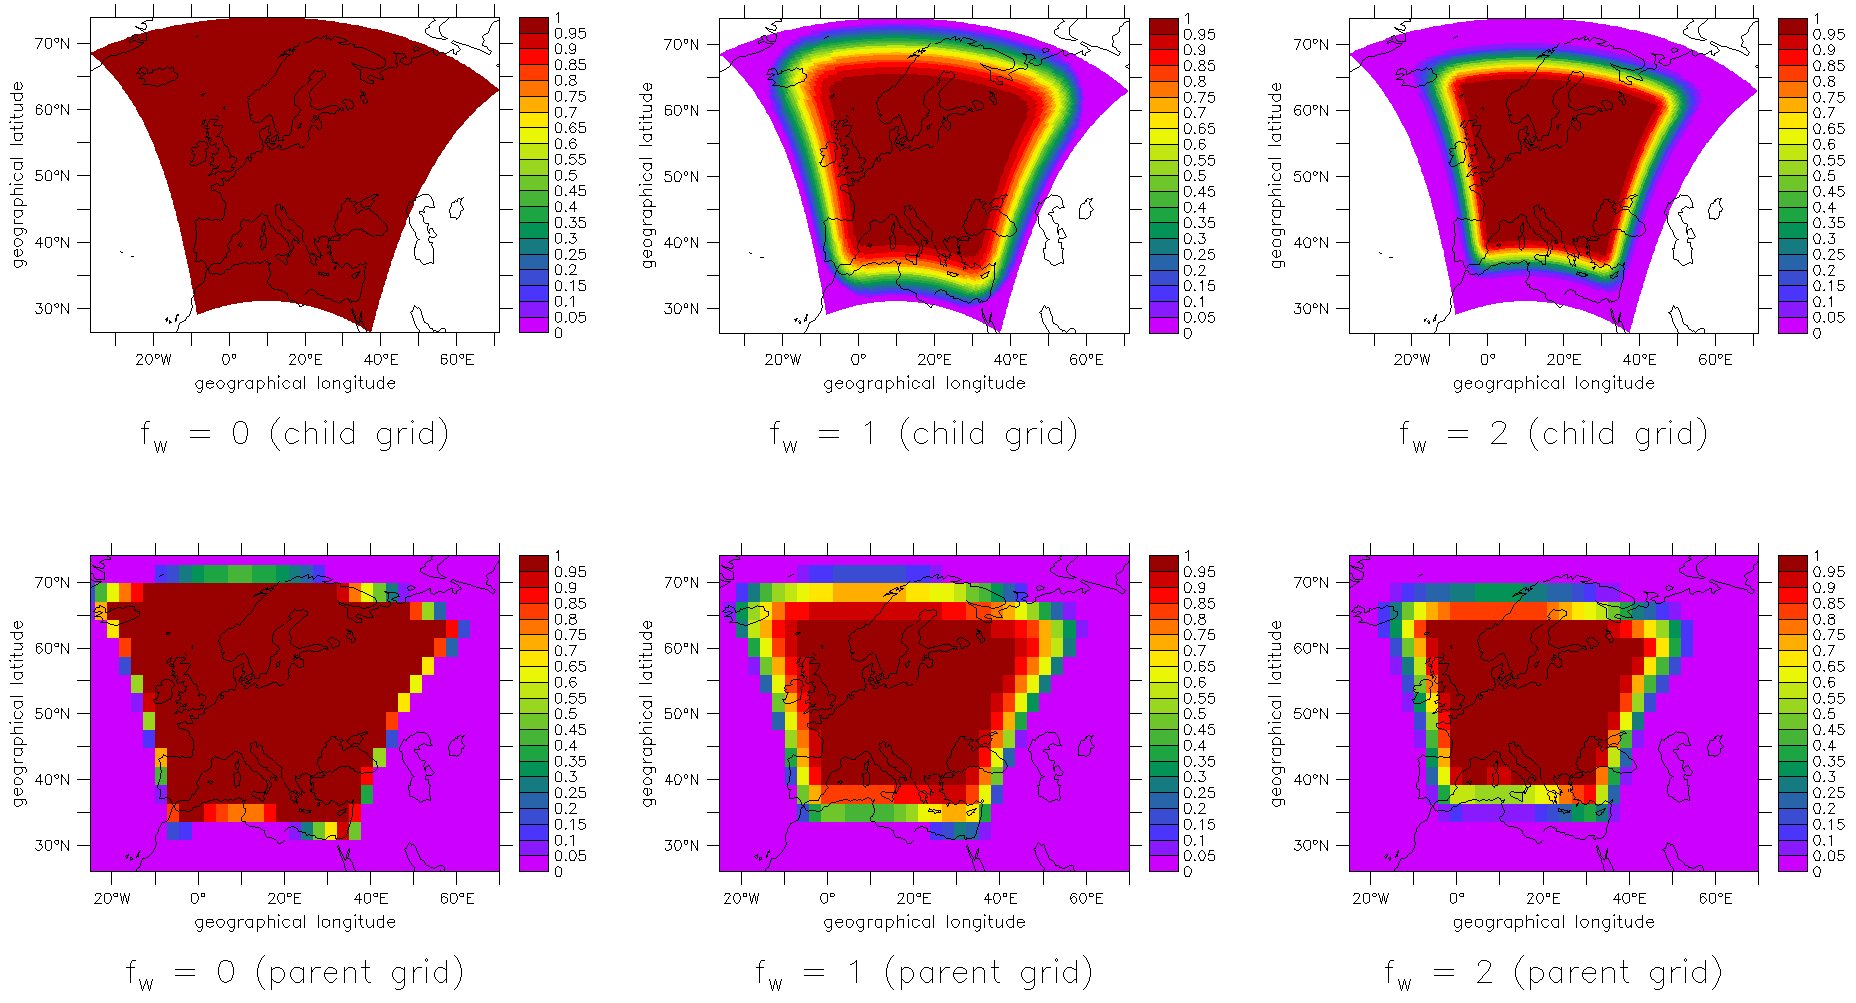
\includegraphics[width=15cm]{MMDUM_weightfunctions}
\end{center}
\caption{Weight functions ($f_w$, see page \pageref{wf}) for the
different weight types, i.e., {\tt itype\_fw} $=0$ (left), $=1$
 (middle) and $=2$ (right). Upper row: 
 weight functions as calculated on the child grid. Lower
 row: weight functions after transformation to the parent grid.\label{fig:weightfunc}}
\end{figure*}
 This is because the damping zone of the regional model itself
should not be coupled back to the parent, as this is directly influenced
by the parent and thus 
spurious damping or amplifications for 2-way coupled variables can occur. 
The lower row of
Fig.\ \ref{fig:weightfunc} shows
the same weight functions after the transformation to the parent grid.
%\end{itemize}
\item \verb|itype_VI| gives the vertical remapping type. At the moment
only \verb|itype_VI=1| is implemented, i.e., vertical remapping via NREGRID.
\item \verb|RCF| and \verb|RCF_IN| are used to avoid rounding errors in the
calculation of the grid longitudes and latitudes. In the COSMO model the
longitude of a grid point with $i$ ($lon(i)$) in the local domain is
calculated by  
\begin{verbatim}
itot = isubpos(my_cart_id,1) - nboundlines - 1
lon(i) = startlon_tot + (itot + i) * dlon
\end{verbatim}
This can lead to rounding errors. Therefore this calculation is shifted to
integer arithmetic to minimize these errors:
\begin{verbatim}
itot = isubpos(my_cart_id,1) - nboundlines - 1
istartlon = NINT(startlon_tot * RCF)
idlon     = NINT(dlon         * RCF)
itmp      = istartlon + (itot+i) * idlon
lon(i)    = REAL(itmp,dp) / RCF
\end{verbatim}
Thus, \verb|RCF| and \verb|RCF_IN| should give as many decimals
as \verb|dlon| and \verb|dlon_in| have significant decimals.
For example, a grid with \verb|dlon = 0.36| should get an \verb|RCF|
of \verb|100|. 
\item  \verb|ldiagonly| is a switch, that can be used, if only fields for
diagnostics are coupled. In this case the surface pressure of the parent
is used for the backtransition and the iteration of the calculation of
the vertical
profiles of humidity/ water variables and temperature to calculate the
surface pressure is skipped.
\end{itemize} %i2-
\item \verb|boxarea_out| provides the area of each grid box of the {\it out-grid}.

\item \verb|l_shortcut| is a switch implemented for testing purposes. If 
\verb|.TRUE.| the fields as received from the parent are coupled directly back
to the parent.
\item The 2D {\footnotesize POINTER} array \verb|iterps| and the
arrays \verb|npsiter1|, \verb|npsiter01|, \verb|npsiter001|,
 \verb|npsiter0001|, and \verb|npsitermax| have been used during the development 
of the backward coupling. The \verb|npsiterXX| arrays provide the iteration
 number after which the surface pressure fields deviated less
 than \verb|1. Pa|, \verb|0.1 Pa|, \verb|0.01 Pa| or \verb|0.001 Pa| from the
 surface pressure fields of the previous iteration step,
 respectively. \verb|iterps| contains the surface pressure after each
 iteration step, where \verb|nitermax| gives the number of possible iterations.

\end{itemize}
\subsubsection{mmd2way\_child\_setup}
The only parent-to-child coupling specific part in \verb|mmd2way_child_setup|
is that at the end of the subroutine the parameter \verb|nitermax| is set. It 
depends on the parent. \verb|nitermax| gives the maximal number of
iterations  
between the calculation of the surface pressure and the vertical profiles of 
 temperature, water vapour, cloud
water and cloud ice, which is required during the vertical remapping.
\subsubsection{mmd2way\_child\_init\_memory}
In \verb|mmd2way_child_init_memory| not only the preparations for
both, the 1-way and 
the 2-way coupling, are performed. In addition:
\begin{enumerate}
\item Two {\it channel objects} are created: the
first one contains the horizontal weight function (\verb|fw|)
 as calculated on the child grid. The other contains the respective 
\verb|mask|, which is \verb|1| where \verb|fw| is larger
than \verb|0.9999._dp|.
\item  The MMD library  subroutine \verb|MMDC_C_Get_ParDataArray_Name|
is called. This subroutine organizes the transfer of the information about the
 {\it coupled fields} required by the child for the parent-to-child
 coupling. 
 Its only parameter is the number of {\it coupled fields} requested by the
 parent (\verb|PD_NUM|).
\item The content of the child specific parent \verb|&CPL_PAR_CHILD|
 namelist is broadcasted using the MMD library
 subroutine \verb|MMD_Inter_Bcast|. Subsequently, the parameters are saved in
 the respective local variables, i.e., \verb|lgrhum|, \verb|i_rmy_px|, 
\verb|pcontol_fi|, \verb|itype_fw|, \verb|icosexp|, \verb|idamprel|, 
\verb|itype_VI|, \verb|lcpl_global_start|, \verb|RCF|, \verb|RCF_IN| and
\verb|ldiagonly|. 
\item The height of the damping layer (\verb|rdheight|) is defined in height 
 coordinates. For the coupling this height is required to be in pressure
 coordinates (\verb|p_rdheight|), which is calculated here. Additionally, the
 index \verb|chi_kmin| of the highest layer below the damping layer 
is determined. \verb|p_rdheight| is sent to the parent using the MMD 
library routine \verb|MMD_Sent_to_Parent|. Subsequently, the parent
 sends back the corresponding vertical index of this height (\verb|par_kmin|)
in the parent grid. This is required for the memory allocation of the 
{\it exchange fields}.
\item The subroutine \verb|exchange_grids| serves four purposes: (1)
 it determines the part of the child domain, which is fed back to the
 parent; (2) the weight 
 function is calculated, (3) the coupling area for the 1-way
 coupling is set up (as described on page \pageref{SR:exchange_grids})
and (4) the {\footnotesize LOGICAL}
 switch \verb|L_gridrotParenteqChild|
is set.

\begin{enumerate}
\item[(1)] The local COSMO model field \verb|rmy| containing the relaxation
coefficients at the borders of the child model domain is gathered and
used for the definition of a global mask. \verb|rmy| is zero outside
the relaxation zone, whereas it is larger zero in the relaxation
zone. Thus, the indices marking where in the global field the relaxation
coefficients become zero (\verb|is_p3|, \verb|js_p3|, \verb|ie_p3|
and \verb|je_p3|) are determined. These indices are similar to the
usual  COSMO model notation, as (\verb|istart|,  \verb|jstart|) marks
the lower left corner of the local COSMO domain,
(\verb|is_p3|, \verb|js_p3|) mark the lower left corner of the
coupling domain and (\verb|ie_p3|, \verb|je_p3|) describe the upper
right corner of the domain coupled back to the parent model. 
If in addition to the relaxation zone further points should be
excluded from the coupling region, the index quadruple is adjusted by
adding / substracting the respective number of additional points
(namelist parameter \verb|i_rmy_px|). In the global field \verb|rmy_glob|
the grid boxes excluded from the coupling are filled with dummy values
larger than zero, indicating that they do not contribute to the data
coupled back to the parent. In the end the global
field \verb|rmy_glob| is distributed again to the local tasks yielding
the local decomposed field \verb|rmy_loc|. This is used in 
\verb|DEFINE_REDUCED_BM_GRID| to determine the local start and end
indices for the data entering the remapping routines.

\item[(2)] The available weight functions have been discussed earlier
(see page \pageref{descript:itype_fw}). First, the weight function is
calculated for a global field \verb|fw_glob|. Afterwards the global
weight function field is distributed to yield the local decomposed
weight function field \verb|fw|.
\item[(3)] The {\footnotesize LOGICAL} switch 
\verb|L_gridrotParenteqChild| indicates, if the grids of the parent and the
child are identically rotated. If ECHAM is the parent, this
switch is always \verb|.FALSE.|, as ECHAM uses a Gaussen grid and
therefore the parent and child grids do not match anyway. For
the COSMO model as parent 
model, it is tested whether \verb|pollon|, \verb|polgam|
and \verb|pollat| are the same for both models. In this case 
\verb|L_gridrotParenteqChild| will be set \verb|.TRUE.|.
Alternatively, \verb|L_gridrotParenteqChild| will be set \verb|.TRUE.|
if \verb|pollat_in == pollat| and one of \verb|pollon_in|
and \verb|polgam_in| is \verb|0._dp| and the 
other \verb|180._dp|, while \verb|pollon| and \verb|polgam| are
defined the other way round. In this case the grid rotation is also
the same.
\end{enumerate}


\item In the subroutine \verb|parent_assign_ParData| the definition of the 
{\it coupled fields} takes place. Therefore, first \verb|ParData| is allocated
to the number of {\it exchanged fields} (\verb|PD_NUM|) plus a maximum number of
{\it additional fields}, which might be required for the remapping procedure.
At this point only the number of namelist requested fields is known,
not the fields themselves, therefore the exact number of {\it
additional fields} is not known and therefore the maximum number has
to be used.  In an endless loop (loop index \verb|ii|) calling the MMD library
function  
\verb|MMD_C_GetNextParArray|, the name of the {\it channel} 
(\verb|ParData(ii)%name%CHA|) and the {\it
channel object} (\verb|ParData(ii)%name%OBJ|) of the coupled child 
field, its representation (\verb|ParData(ii)%repr|), the
interpolation method (\verb|ParData(ii)%interpM|) and the
information, if the unit of the field should be sent
(\verb|ParData(ii)%l_SentUnit|) are saved. 
For the special case that an array is to be coupled, which is defined by 
MMD2WAY\_CHILD itself, a special action is required during the 
child-to-parent coupling. Therefore the index of this field in the 
\verb|ParData| array  has to be saved in the derived type variable 
(\verb|CplData|). Thus, in this case  \verb|CplData(ii)%scn| is set to the 
current loop index \verb|ii|.
\item In the subroutine \verb|match_parent_grid| the weights for the
remapping during the backward coupling are calculated. 
First, the longitudes (\verb|rlons|) and latitudes (\verb|rlats|) of the grid
mid points of the rotated {\it out-grid} are calculated, and afterwards the
subroutine \verb|CALC_backward_WEIGHTS| is called. Before the weights can be
calculated in subroutine \verb|CALC_backward_WEIGHTS|, the grids for the
remapping need to be defined. 
\begin{itemize}
\item {\bf definition of reduced child grid}\\
As discussed before, not the full child grid is used for the backward
coupling. Thus first, the start grid of the remapping, the so-called
``reduced basemodel grid'', needs to be defined as geo-hybrid grid. This is
done in the subroutine 
\verb|define_reduced_BM_grid|. The reduction of the grid is twofold: 
\begin{enumerate}
\item  In the \label{page:addframe}
horizontal the points of the relaxation zone plus the ``additional frame'' as
given by the namelist parameter \verb|i_rmy_px| are excluded. In case of a 
very broad additional frame, it can happen, that the local domains located at
the border of the full COSMO domain do not contribute any grid boxes 
to the backward coupling.  In this case the {\footnotesize LOGICAL
}\verb|l_overlap| is 
set to \verb|.FALSE.| for an easier handling of  ``empty'' or ``non-active''
local domains. 
\item  The vertical
dimension can be reduced by the damping zone at the model top. Its length 
is thus given by \verb|nlev+1-chi_kmin+1|.
\end{enumerate}
For the special case that the child and the parent are both COSMO instances
and their grids are rotated identically (indicated by the {\footnotesize LOGICAL }
\verb|L_gridrotParenteqChild|) the subroutine \verb|define_rotred_BM_grid| is
called instead of the subroutine \verb|define_reduced_BM_grid|.
This subroutine takes advantage of the identical rotation, which helps  
to avoid additional numerical inaccuracies by additional grid rotations.

For the data processing this 3D grid and a 
horizontal grid are required. Thus in addition to the reduced child
grid (\verb|cgrid|), the reduced horizontal child grid (\verb|chgrid|) is
defined by using the GRID subroutines \verb|COPY_GEOHYBGRID| and 
\verb|SWITCH_GEOHYBGRID|.                 
\item {\bf definition of the {\it out-grid}}\\
The definition of the 3D and the horizonal {\it out-grids} (\verb|pgrid| and
\verb|phgrid|) follows the same lines as the definition of the reduced child
grid. Here, the {\it in-grid} information as required for the 1-way coupling 
is used. The length of the vertical dimension is given by 
%\begin{eqnarray}
\verb|ke_int  =  ke_in - par_kmin + 1|.
%\end{eqnarray}
\item{\bf calculation of backward weights}\\
For the horizontal remapping, SCRIP, as provided in the generic submodel
 GRID, is used. Thus, the reduced child and parent grids, are used to
define the grid information required by the SCRIP software. This needs to be
 done for each field individually, as in principle different remapping
 algorithms can be chosen for each field individually. 
The GRID subroutine \verb|CALC_SCRIPDATA| extracts the information required
by SCRIP from the geo-hybrid grids \verb|cgrid| and \verb|pgrid|.
These data are saved in the variable \verb|ParData(ii)%PSD|.
Subsequently, these are used to calculate the weights for the horizontal
 remapping (subroutine call to \verb|CALC_SCRIP_WEIGHTS|).
For later use, the index \verb|fw_SD_ID| is set to the index of the first
{\it coupled field} requiring conservative remapping. 
\item{\bf remapping of the weight function}\\
As all information required for a horizontal remapping is now available, 
in a last step, the horizontal weight function \verb|fw| is remapped to
the {\it out-grid} yielding the remapped horizontal weight
function \verb|fw_int|. 
If the index \verb|fw_SD_ID| is set, the remapping weights have already been
calculated and can be used for the weight function remapping, otherwise,
they are calculated here.
By calling the subroutine \verb|RGTOOL_CONVERT_DAT2VAR| \verb|fw| is converted
to the 1D format required by GRID. Afterwards, the remapping proceeds by
calling \verb|SCRIP_CONTROL|. Finally, the remapped data are converted from the
GRID 1D format to yield \verb|fw_int|.
\end{itemize}


\item {\bf Setup\_ParData\_exchange}\\
The subroutine \verb|Setup_ParData_exchange| serves two purposes:
\begin{enumerate}
\item It provides the data to calculate the IndexList for the data
backtransition and receives the IndexList from the parent. This works in
the same way as described for \verb|Setup_data_exchange_with_parent| for the
data exchange between parent and child.
\item The information which fraction of the {\it out-grid} is overlapped by the
local reduced child grid is retrieved. Principally, the SCRIP data
contains the information
(\verb|ParData(conserv_idx)%PSD%wghts%dstfrac|).
As the SCRIP data is in the GRID 1d format, it needs to be de-alined
to yield the required 2d data field \verb|fractions|.
In the subroutine 
\verb|determine_fractions| the destination fraction of a conservativly
remapped field is de-alined to yield a 2D array defined on the {\it out-grid}.
\end{enumerate}
\item  {\bf parent\_make\_representations}\\
In this subroutine the {\it representation}
for the {\it channel objects} defined on the {\it out-grid} are build. \label{makeprepr}
First, six {\it dimenions} are defined:
\begin{itemize}
\item the first horizontal dimension \verb|'MMDOUT_ie'| 
(dimension ID: \verb|DIMID_POUT_IE|),
\item the second horizontal dimension \verb|'MMDOUT_je'| 
(dimension ID: \verb|DIMID_POUT_JE|),
\item the vertical dimension of the remapped field \verb|'MMDOUT_kmin'| of
length \verb|ke_int| (dimension ID: \verb|DIMID_POUT_KMIN|),
\item the vertical dimension for the interfaces of the remapped
field \verb|'MMDOUT_kminp1'| of 
length \verb|ke_int+1| (dimension ID: \verb|DIMID_POUT_KMINp1|),
\item the vertical dimension of the horizontally remapped
field \verb|'MMDOUT_hint'| of
length \verb|ke_hint = ke - chi_kmin + 1 | (dimension
ID: \verb|DIMID_POUT_HINT|),
\item the vertical dimension for the interfaces of the remapped
field \verb|'MMDOUT_hintp1'| of 
length \verb|ke_hint+1| (dimension ID: \verb|DIMID_POUT_hintp1|).
\end{itemize}
Subsequently, by using these {\it dimensions}, the following {\it
representations} with the decomposition type \verb|DC_MMD_OUT| are
defined:
\begin{itemize}
\item \verb|REPR_POUT_2D| (dimension ID: \verb|REPR_POUT_2D|): the horizontal
{\it out-grid}, defined by the dimensions \verb|'MMDOUT_ie'|
and  \verb|'MMDOUT_je'|.
\item \verb|REPR_POUT_3D_MID| (dimension ID: \verb|REPR_POUT_3D_MID|): 
the {\it out-grid} defined on the grid mid-points, i.e., by the
dimensions \verb|'MMDOUT_ie'|, \verb|'MMDOUT_je'| and \verb|'MMDOUT_kmin'|.
\item \verb|REPR_POUT_3D_INT| (dimension ID: \verb|REPR_POUT_3D_INT|): 
the {\it out-grid} horizontally defined on the grid mid-points,  vertically on the
interfaces, i.e., by the
dimensions \verb|'MMDOUT_ie'|, \verb|'MMDOUT_je'| and \verb|'MMDOUT_kminp1'|.
\item \verb|REPR_PHOUT_3D_MID| (dimension ID: \verb|REPR_PHOUT_3D_MID|): 
the horizontally remapped grid defined on the grid mid-points, i.e., by the
dimensions \verb|'MMDOUT_ie'|, \verb|'MMDOUT_je'| and \verb|'MMDOUT_hint'|.
\item \verb|REPR_PHOUT_3D_INT| (dimension ID: \verb|REPR_PHOUT_3D_INT|): 
the horizontally remapped grid, horizontally defined on the grid mid-points,
vertically defined on the interfaces, i.e., by the
dimensions \verb|'MMDOUT_ie'|, \verb|'MMDOUT_je'| and \verb|'MMDOUT_hintp1'|.
\end{itemize}
For the same five combinations of {\it dimensions} additional five {\it
representations} 
are defined using the decomposition type \verb|DC_MMD_OUTACC|.
Thus, the five respresentations \verb|REPR_POUTACC_2D|, 
\verb|REPR_POUTACC_3D_MID|, \verb|REPR_POUTACC_3D_INT|, 
\verb|REPR_PHOUTACC_3D_MID| and \verb|REPR_PHOUTACC_3D_INT| are defined.
``ACC'' indicates that these objects need to be
``accumulated'' when written to a file. 
Normally, the fields on the COSMO grid consist of the so-called ``inner
domain'' and a halo-region. The inner domains are disjunct on all PEs. Thus,
for the output the content of the inner domains of each task is dumped to the
 output file.
This is different for the fields remapped to the {\it out-grid}. Here, each task
contains the fraction, which was covered by the reduced child grid. Thus on
output, to yield the full field, all fractional contributions of the single
tasks need to be summed up. This is invoked by the decomposition
type  \verb|DC_MMD_OUTACC|. 
\item {\bf parent\_set\_ParData}\\
In the subroutine \verb|parent_set_ParData|, the {\it channel objects}
for the back transition are defined. These are:
\begin{itemize}
\item the interpolated weight function \verb|fw_int|,
\item the \verb|fractions| of the {\it out-grid} covered by the local task,
\item the arrays for the diagnostics of the surface pressure iteration, and
\item the area of the {\it out-grid} grid boxes \verb|boxarea_out|. 
\end{itemize}

In a loop over all {\it coupled field}s 
\begin{enumerate}
\item the indices of variables, which require special treatment during
the remapping are saved.
\item depending on the representation of the field, the new {\it channel
objects} for the backtransition, i.e., \verb|ParData(ii)%ptr_hint| and
 \verb|ParData(ii)%ptr_int| are defined, using the above mentioned
 {\it representations}.
\item the \verb|rank|, \verb|AXIS| string and the length of the local
 dimensions \verb|ldimlen| are inquired by
 calling \verb|get_representation_info|.
\item by calling the MMD library subroutine \verb|MMD_C_Set_ParDataArray|,
the memory and the dimension information are provided to the MMD library.
\end{enumerate}
For later use, during this loop an index of a field remapped with
interpolation method 1 (\verb|idx_int1|) and of a field which {\it coupled
field}  is of
representation \verb|GP_3D_MID| (index \verb|idx_p_3d|) is saved.

Finally, additional fields are added to the list of fields that need to be
remapped. Basically, these are all variables which are required for
the adjustment of the vertical
profiles, i.e., 
\begin{itemize}
\item for ECHAM as parent instance: the surface pressure \verb|'PS'|, the surface geopotential 
\verb|'FIS'|, the control level geopotential \verb|'FIC'|, the 3D pressure field \verb|'PRES'|, the 3D
temperature field \verb|'T'|, water vapour \verb|'QV'| and cloud
 water \verb|'QC'|
\item for COSMO as parent instance: the 3D
temperature field \verb|'T'|, the surface pressure \verb|'PS'|, the surface
temperature \verb|'T_S'|, the height of the surface \verb|'HSURF'| and the 3D
deviation of the pressure field \verb|'PP'|.
\end{itemize}
These fields are added by calling the
subroutine \verb|add_parent_list_element|.
\item Finally, in the subroutine \verb|init_parent_coupling|, the {\footnotesize POINTERs} to
the child fields of the {\it coupled field}s are acquired. 
In the simplest case, this is achieved by calling \verb|get_channel_object|.
Additionally, if the unit of the {\it coupled field} is required by the parent
model, the unit is sent here.

In some very specific cases the memory needs to be allocated in MMD2WAY\_CHILD
itself, which is done by first finding the correct representation ID  by
calling the CHANNEL subroutine \verb|get_representation_info| using the
representation as sent by the parent \verb|ParData(ii)%repr|.
Secondly, the memory is allocated by calling \verb|new_channel_object| using
the representation ID.

Finally, for both cases the information, if the {\it coupled} child
 {\it field}
depends on time (\verb|ParData(ii)%itimedep|), is set by inquiring, whether
the representation of the child field contains the timelevel dimension
ID \verb|DIMID_TLV|.
\end{enumerate}

\subsubsection{mmd2way\_child\_init\_loop }
In \verb|mmd2way_child_init_loop| no backward coupling specific tasks
need to be performed. 
\subsubsection{mmd2way\_child\_global\_end}
Apart from the exchange of the TIMER information, which is already required
for the 1-way coupling, in \verb|mmd2way_child_global_end| the remapping 
of the fields to the {\it out-grid} and the data exchange from the child to the
parent takes place. The latter consists simply of the call of the MMD library
routine \verb|MMD_C_FillBuffer|.
However, the subroutine \verb|interpol_parent_data| contains the full
machinery for the remapping of the child fields to the {\it out-grid}.
Chronologically, in the subroutine \verb|interpol_parent_data| in a
loop over the {\it coupling fields}
\begin{enumerate}
\item the vertical extend of each field is determined by setting the
two indices \verb|kkmin| and \verb|kkmax|. For a 2D field both indices
are \verb|1|, for a 3D field is \verb|kkmin = chi_kmin|, i.e., the
first level below the damping layer, and 
\verb|kkmax = SIZE(ParData(ii)%ptr_ori,3)|,
i.e., the vertical dimension of the {\it coupled field}.
\item the {\footnotesize POINTER} to the COSMO field, that should be coupled is
associated. For the variables, which require specifically
precalculated fields and not 
the original COSMO data the {\footnotesize POINTER} \verb|PTR| is set
to this specific 
field, otherwise \verb|PTR| is set generically to the {\it coupled field}
assigning automatically the region, that should be coupled, i.e.,
reduced to the reduced horizontal domain
(\verb|iis:iie|, \verb|jjs:jje|),
the reduced height (\verb|kkmin:kkmax|) and the correct timelevel 
(\verb|tlev:tlev|).
The fields requiring specific treatment are
\begin{itemize}
\item the wind components. In case of the COSMO-EMAC coupling the wind components must be calculated on the cell centers prior to the horizontal interpolation.
\item the specific field \verb|hsurf_full| in case of COSMO-COSMO coupling.
\item the surface pressure,
\item some additional fields required for the surface pressure
iteration during the  vertical remapping.
\end{itemize}
\item the data is transformed to the
GRID internal 1D format using the GRID
subroutine \verb|RGTOOL_CONVERT_DAT2VAR|, 
 if the {\footnotesize POINTER} is associated,.
Afterwards, the horizontal remapping proceeds within the subroutine 
\verb|SCRIP_CONTROL|. This subroutine hands back the remapped field in
the 1D GRID format. This variable is transferred back by calling the
GRID subroutine \verb|RGTOOL_CONVERT|, which result (\verb|dat|) is
the horizontally remapped field \verb|ParData(ii)%ptr_hint|.
Additionally to the data transformation, the intermediate
3D grid \verb|intgrid|, i.e., the grid on
which \verb|ParData(ii)%ptr_hint| is defined (i.e., horizontally equal
to the {\it out-grid} and vertically still the reduced COSMO model grid),
 also output by the subroutine \verb|SCRIP_CONTROL| is saved in the
variable \verb|phgrid_3d|, as this is required for the vertical regridding.
\end{enumerate}
Last but not least, the vertical remapping takes
 place. The sequence of surface pressure adaptation and vertical
 remapping is adopted from the respective procedures in INT2LM.
Different algorithms are called depending on the parent
 instance:
\begin{itemize}
\item ECHAM is parent instance: {\bf vert\_interpol\_lm2echam}
\begin{itemize}
\item First,  a {\footnotesize LOGICAL }mask (\verb|lcalc|) is defined, which is \verb|.TRUE.|
if the horizontal weight function is larger than zero. This mask is used
later on, to limit the calculations to those grid boxes, where
meaningful values exist.
\item Second, the iteration of the surface pressure takes place. This step
is skipped, if \verb|ldiagonly=.TRUE.|. In the latter case the
original surface pressure of the parent model is used.
At the beginning of the iteration a first guess surface pressure is
calculated using the subroutine \verb|CALC_ALPS_1| which works in a
similar way as \verb|calc_alps_1| in INT2LM. 
Then, in an iteration loop, the vertical profiles for temperature, water
vapour, cloud water and cloud ice, are calculated based on the current
surface pressure guess. Based on this profiles a new surface pressure
is calculated by the subroutine \verb|calc_alps_2|, 
with which, in the next cycle, new vertical profiles are
calculated. For diagnostic purposes each step of the iterated surface
pressure is saved in a {\it channel object} and the differences between
the surface pressures of the individual iteration steps are analysed.
\item After the iteration, the vertical profiles of all {\it exchange fields}
are calculated using  the ``final'' surface pressure.
\end{itemize}
The vertical profiles are calculated using the
subroutine \verb|vert_c2p_ncinterpol|. Within this subroutine NREGRID
as provided by the GRID submodel is used to perform the vertical
remapping.
First, the definitions of the geo-hybrid grids of the in-coming grid
is adapted to the needs of only vertical regridding. Second,
the surface pressure in the grid definition is set by calling the
GRID subroutine \verb|SET_SURFACE_PRESSURE|. Afterwards, the data is
converted to the 1D GRID format by the GRID subroutine 
\verb|RGTOOL_CONVERT_DAT2VAR|. The vertical remapping proceeds within
the subroutine \verb|REGRID_CONTROL|. Finally, the INTENT(out)
variable containing the fully remapped field is filled, after the
backtransition into the full three dimensional data field using the
GRID subroutine \verb|RGTOOL_CONVERT|.

\item COSMO is parent instance: {\bf vert\_interpol\_lm2lm}\\
This subroutine is a copy of the INT2LM
subroutine \verb|org_vert_inter_lm|,
which was adapted to the backward coupling of the data.
\begin{itemize}
\item First, the reference atmosphere for the intermediate (only
horizontally remapped) data is calculated (here
the \verb|hsurf_full| field is required to avoid decomposition
dependent results).
\item Secondly, after computation of some helper variables, the pressure
deviation field is vertically remapped using the
subroutine \verb|vert_interp|. This subroutine is again a copy of the
INT2LM routine and performs a spline interpolation of the vertical
profiles.
\item Third, the vertical velocity is remapped vertically.
\item Next, within a loop, all other variables are 
remapped vertically to the parent grid.
\item In the end, the pressure deviation field is corrected, taking the new
vertical profiles into account.
\end{itemize}

\end{itemize}
\subsubsection{mmd2way\_child\_write\_output}
As explained for the subroutine \verb|parent_make_representation|
(page \ \pageref{makeprepr}) the {\it channel objects} of
decomposition type \verb|DC_MMD_OUTACC| are summed up when the respective
{\it channel objects} are gathered.
Thus the fields need to be multiplied by the fraction of the {\it out-grid},
which is covered by the child grid on the respective task before the call to
the MESSy output routines. After output was performed, 
 they must be divided by the fraction to yield back the original fields.
This is done in the subroutine \verb|mmd2way_child_write_output|.

\subsubsection{mmd2way\_child\_read\_restart}
This subroutine calls \verb|mmd2way_child_write_output| for the
conversion of the fields into fractions.
\subsubsection{mmd2way\_child\_write\_restart}
This subroutine calls \verb|mmd2way_child_write_output| for the summation of
the fields.
\subsubsection{mmd2way\_child\_free\_memory}
In \verb|mmd2way_child_free_memory| the memory required for the backward
coupling is deallocated, i.e., \verb|p_fis|, \verb|hsurf_full|
and \verb|ParData|, in addition to the deallocations required for the
1-way coupling. 

\section{Changes in INT2LM code required for the MESSy submodel INT2COSMO}
\label{sec:INT2COSMOcode}

Most changes to the INT2LM code have been embedded in the preprocessor
directive {\tt \large I2CINC} 
({\tt \large I}{\footnotesize NT}{\tt \large 2C}{\footnotesize OSMO} 
{\tt \large IN C}{\footnotesize OSMO}).
However, in order to improve the 2-way coupling additional extensions
have been added using the preprocessor directive  {\tt \large MESSYTWOWAY}. 
In this section the changes and the reasons for them are listed for each code 
file. The files are listed in alphabetical order.
The changes refer to INT2LM version 2.00.
\subsection{data\_fields\_lm.f90 /data\_fields\_in.f90 }
As all INT2COSMO fields are allocated as MESSy {\it channel objects},
 they have to be declared as {\footnotesize POINTER}s, instead of 
{\footnotesize ALLOCATABLE ARRAYs}. 
The definitions are replaced throughout the module for all {\footnotesize REAL} 
arrays.

In \verb|data_fields_lm.f90| some extra fields are defined:
\begin{itemize}
\item  \verb|zfi_fl|, \verb|zhi_fl|, \verb|zps1_lm|,
 \verb|zkzgr|: in the off-line 
 INT2LM these fields are locally defined intermediate variables, which are
used during the remapping. In INT2COSMO these fields are also 
 required for the remapping of the {\it additional fields}. 
Therefore, they are declared in \verb|data_fields_lm.f90| and allocated as
 {\it channel objects} in \verb|messy_I2CINC_channel_alloc_lm|.
\item \verb|oromem_lm|: this field is required in the subroutine 
\verb|external_data.f90|. Here,
 the orography or better the surface height at the first call of
 INT2LM must be saved and used in 
 the next calls, otherwise the results of INT2COSMO could depend on the restart
 frequency depending on the parent.
\item \verb|geolon_lm, geolat_lm, geoloni_lm, geolati_lm|: 
longitude and latitude fields in geographical coordinates
 for the INT2COSMO fields. They are required for the definition of
 the geo-hybrid INT2COSMO grids, if conservative remapping is chosen.
\item \verb|lon_lm, lat_lm, loni_lm, lati_lm| contain
 the (interface) longitude and latitude fields in rotated coordinates
 for the INT2COSMO fields. They are required for the definition of
 the geo-hybrid INT2COSMO grids, if conservative remapping is chosen.
\item \verb|psiter01_lm, psiter02_lm, psiter03_lm, psiter04_lm|
and \verb|psiter05_lm|. These fields are defined for diagnostic output
during the development of the 2-way coupling. Thus they only exist, if
the preprocessor directive  { \tt \large MESSYTWOWAY} is active.

\item \verb|fic2_gl, fic3_gl|: these fields are only defined, if
 MESSYTWOWAY is active. They are used for some diagnostic purposes
 during the development of the 2-way coupling.
\end{itemize}

In \verb|data_fields_in.f90| additionally the fields \verb|lon_in|
and \verb|lat_in| are declared, which are required for the definition of
 the geo-hybrid INT2COSMO grids, if conservative remapping is chosen.

\subsection{data\_grid\_in.f90}
In \verb|data_grid_in.f90| the indices for the local decomposed
{\it in-grid} \verb|istartpar_in, iendpar_in, jstartpar_in, jendpar_in|
takes place. These indices are required for the gathering of the
fields defined on the {\it in-grid} if they should be written to the output.
Additionally, the two geo-hybgrids \verb|pingrid| and \verb|pinhgrid|
are declared here. They are required for the conservative remapping.

\subsection{data\_grid\_lm.f90}
Instead of declaring and defining the grid in INT2COSMO independently, 
 the number (\verb|ke_soil_lm|) and 
depths (\verb|czmls_lm| and \verb|czhls_lm|) of the soil layers and the grid 
dimensions and orientation (\verb|dlon|, \verb|dlat|,
 \verb|startlon_tot|, \verb|startlat_tot|, \verb|polgam|, \verb|pollon|,
 \verb|pollat|, \verb|ielm_tot|, \verb|jelm_tot| and  \verb|kelm_tot|) 
 are USEd directly from the COSMO model and renamed to their INT2COSMO names:
\begin{verbatim}
USE data_modelconfig,  ONLY: czmls_lm => czmls, czhls_lm => czhls  &
                           , ke_soil_lm => ke_soil, ielm_tot => ie_tot &
                           , jelm_tot => je_tot, kelm_tot => ke_tot    &
                           , dlon, dlat, pollat, pollon, polgam        &
                           , startlat_tot, startlon_tot                 

\end{verbatim}
Furthermore, four additional index variables are declared, which are
required for  
the grid mapping of the COSMO and the INT2COSMO grid (\verb|istartcos|,
 \verb|iendcos|, \verb|jstartcos| and \verb|jendcos|). The meaning of these
variables is explained in Sect.\ \ref{sec:INT2COSMO}.

Additionally, for MESSy the knowledge of the hybrid grid coefficients
is required during the model initialisation. Therefore the
fields \verb|ak_lm| and \verb|bk_lm| are declared.

Furthermore, for the conservative remapping and the backward coupling
the respective geo-hybrid grids are defined here:
\begin{itemize}
\item \verb|i2cgrid|: the INT2COSMO grid without
halos and full vertical height 
\item \verb|i2chgrid|: the purely horizontal INT2COSMO grid without halos 
\item \verb|i2cUgrid|: staggered U INT2COSMO grid without
halos and full vertical height 
\item \verb|i2cUhgrid|: the purely horizontal staggered U INT2COSMO
grid without halos  
\item \verb|i2cVgrid|: staggered V INT2COSMO grid without
halos and full vertical height 
\item \verb|i2cVhgrid|: the purely horizontal staggered V INT2COSMO
grid without halos.
\end{itemize}
Finally, the respective SCRIP data variables
 (\verb|I2C_SD|, \verb|I2C_U_SD|, and \verb|I2C_V_SD|) and the indices
of the SCRIP data sets (\verb|I2C_SD_ID|, \verb|I2C_U_SD_ID|, and 
\verb|I2C_V_SD_ID|) are declared here.

\subsection{data\_int2lm\_control.f90}
As INT2COSMO and the COSMO model need to be set up in the same way, 
some run control variables are directly used from the COSMO model. Thus those
declarations in \verb|data_int2lm_control.f90| of the 
INT2COSMO namelist parameters, which are also declared for COSMO, are omitted.
\begin{verbatim}
USE data_runcontrol, ONLY: nstop, nstart, llake, lradtopo, lprog_qi  &
                         , itype_calendar, idbg_level, lforest, lsso &
                         , lmulti_layer_lm => lmulti_layer           &
                         , lemiss, lseaice, lstomata                 &
                         , lperi_x, lperi_y, l2dim, itype_aerosol    &
                         , itype_albedo
USE data_io,         ONLY: lbdclim
\end{verbatim}

\subsection{data\_int2lm\_io.f90}
To make INT2COSMO as inherently consistent with the COSMO setup as possible,
the variable \verb|ydate_ini| containing the start date of the simulation
is USEd from the COSMO model module \verb|data_io| instead of being declared 
within this file.

\subsection{data\_int2lm\_parallel.f90}
As INT2COSMO is run in the same parallel environment as the COSMO model,
 most of the
variables are USEd from the COSMO module \verb|data_parallel|, instead of being
defined within INT2COSMO:
\begin{verbatim}
USE data_parallel, ONLY: ldatatypes,lasync_io,nprocx,nprocy,nprocio,nproc,      &
                         num_compute, num_io,ncomm_type,my_world_id,my_cart_id, &
                         my_cart_pos,my_cart_neigh,igroup_world,icomm_world,    &
                         icomm_compute,igroup_cart,icomm_cart,icomm_row,        &
                         iexch_req,imp_reals,imp_grib,imp_integers,imp_byte,    &
                         imp_character,imp_integ_ga,imp_logical,lcompute_pe,lreorder
\end{verbatim}

\subsection{data\_parameters.f90}
To be consistent, the KIND parameters are overwritten by those 
determined within the MESSy submodel \verb|messy_main_constants_mem.f90|.
 \verb|ireals| and \verb|idouble| are set to \verb|dp|, \verb|iintegers| 
is set equal to \verb|i4| and \verb|isingle| to \verb|sp|.

\subsection{external\_data.f90}\label{sec:tech_extdata}
\begin{itemize}
\item The MESSy submodel MMD2WAY\_CHILD calls the subroutine \verb|external_data|
with an additional parameter: \verb|lread|. This {\footnotesize LOGICAL}
indicates whether the external data should be read or not. 
When \verb|lread| is \verb|.FALSE.|, the initialisation of the
{\footnotesize LOGICALs} (indicating the existence of specific variables in the 
external data file) with \verb|.FALSE.| and the subroutine \verb|read_lm_ext| are
not processed. Additionally, \verb|rootdp_mx| must only be set, if data 
was read, i.e., \verb|lread=.TRUE.|.
\item All parameters and variables determining the coarse grid are directly 
exchanged with the server via MMD. Thus the subroutine 
\verb|read_coarse_grid_ext| is not called in INT2COSMO.
The {\footnotesize LOGICALs} \verb|lfis_in| and \verb|lfrla_in| are set to 
\verb|.TRUE.|, according to the fields exchanged during the on-line coupling.

\item The variables \verb|fr_land_in|, \verb|z0_in|, \verb|plcov_in|,
 \verb|plcmx_in|, \verb|plcmn_in|, \verb|rlaimx_in|, \verb|rlaimn_in| and
 \verb|root_in| are not deallocated from INT2COSMO.
In INT2COSMO these variables are {\it channel objects} and as such 
automatically deallocated by the CHANNEL submodel.
\item The allocation of \verb|local_iso_points| and its 
 calculations are only performed at the first call of INT2COSMO.
\item The possibility to remap all variables with the conservative
 remapping provided by GRID was added. Two (hard-coded) additional
 {\footnotesize LOGICALs} determine, whether the external data should
 be remapped using SCRIP.
\begin{itemize}
\item  \verb|l_interp_crl| is used to change from linear interpolation
 (interpolation flag 'L') to conservative remapping. This concerns the
 fields 'FR\_LAND', 'FIS\_IN' and 'HSURF\_IN'.
\item  \verb|l_interp_crm| is used to change from match point
 interpolation (interpolation flag 'M') to conservative
 remapping. This concerns the fields
 'Z0', 'ROOT', 'PLOCV\_MX', 'PLOCV\_MN', 'LAI\_MX' and 'LAI\_MN'.
\end{itemize}
Both switches are experimental. Therefore they are \verb|.FALSE.| by default.

\item As already mentioned for the file \verb|data_fields_in.f90|, it
is important, that the calculation of the fields \verb|hsurf_lm|
and \verb|fis_lm| takes place with the same surface orography in
all time steps. Otherwise the results are restart frequency
dependent. Therefore, 
the variable \verb|oromem_lm| contains a copy of \verb|hsurf_lm| at
the last time step, where external data was actually read. 

\end{itemize}

\subsection{interp\_utilities.f90}
This code file contains all subroutines used for the horizontal remapping.
Thus, for the on-line coupling a subroutine \verb|interp_c| was added,
which links to the MESSy submodel GRID providing the conservative remapping.


\subsection{setup\_int2lm.f90}
\begin{itemize}
\item The memory allocation for the fields of INT2COSMO is modified (compared
to INT2LM) from allocating the fields to defining {\it channel objects}
 for them.
For the definition of {\it channel objects} the {\it representations} of these 
objects must be specified. 
Within the subroutines \verb|messy_I2CINC_channel_make_MMDC4|, 
\verb|messy_I2CINC_channel_alloc_lm|  and 
\verb|messy_I2CINC_channel_alloc_cg|, 
which are called 
from \verb|setup_int2lm|, the {\it dimensions} and {\it representations}
required for the {\it channel objects} are created and the {\it
channel objects} are defined. 

\item As INT2COSMO uses the parallelisation of the COSMO model, the subroutines
\verb|init_environment|, \verb|init_procgrid|, \verb| mpe_io_init| and
 \verb|mpe_io_reconfig| are skipped.
On the other hand, the arrays \verb|isubpos_in|
and \verb|isubpos_in_red| are allocated and initialised here. They are
required for the on-line coupling to address the input
fields correctly.
\item INT2LM offers the possibility to measure the timing of different phases of
the remapping process. Most of the required calls occur in subroutines
and in the main program, which are skipped in INT2COSMO. Therefore, the 
initialisation of the timing located in \verb|setup_int2lm| is skipped for 
INT2COSMO too.
\item The subroutine \verb|clm_setup| provides utilities for the
setup of climate simulations. However, as this relies on input files
not available for the on-line coupling this subroutine is skipped.
\item The debug output file is renamed to \verb|'YUDEBUG_i2cinc'|, because the 
COSMO model also writes a file named \verb|'YUDEBUG'|.
\item At the end of the subroutine, the length of the sent buffer 
(\verb|isendbuflen|) is determined.
The calculation relies on the knowledge of the decomposition of the INT2COSMO
grid. In INT2LM the local domains are equally dimensioned, depending
on the total number of grid boxes (\verb|ielm_tot| or \verb|jelm_tot|) plus the 
boundary lines (\verb|nboundlines|) and the number of processes (\verb|nprocx|
 or \verb|nprocy|). This is no longer correct in INT2COSMO.
Here, the local domain size also depends on  the COSMO number of boundary
lines (\verb|nboundlines_cosmo|). This is taken into account in the 
calculation of \verb|isendbuflen|.
\end{itemize}

\subsection{src\_2d\_fields.f90}
\verb|t_so_lm| is defined in the vertical from \verb|0:ke_soil+1|. As {\it 
channel objects} can only be allocated starting by 1, due to the used 
{\footnotesize POINTER} arithmetic, \verb|t_so_lm| is allocated in the vertical
by \verb|1:ke_soil+2|. This has to be taken into account for the calculation
of \verb|t_so_lm|. For instance,
\begin{verbatim}
#ifndef I2CINC
          t_so_lm(i,j,0) = t_s_lm(i,j)
        ELSE
          t_so_lm(i,j,0) = undef
#else
          t_so_lm(i,j,1) = t_s_lm(i,j)
        ELSE
          t_so_lm(i,j,1) = undef
#endif
\end{verbatim}
All places, where \verb|t_so_lm| is calculated or used, are changed 
accordingly.

Additionally, the option of conservative remapping has been added for 
\verb|'w_so_rel'|.

\subsection{src\_cleanup.f90}
In INT2COSMO the subroutine \verb|free_memory| is almost completely skipped, 
as all fields deallocated in INT2LM in this subroutine are declared as 
{\it channel objects} and thus
deallocated automatically within the CHANNEL submodel. Only the three 
{\footnotesize LOGICAL} (land-sea) masks
\verb|lolp_lm|, \verb|lolp_in| and \verb|lmask_lm| 
are allocated manually in \verb|messy_I2CINC_channel_alloc_*| as they
 can not be defined directly as {\it channel objects} and thus are still 
 deallocated within \verb|free_memory|. 

\subsection{src\_coarse\_interpol.f90}
\begin{itemize}
\item In case of INT2COSMO the on-line exchanged data is always handled
similar to \verb|'ncdf'| data. 
Thus, for the undefined values always the undef flag
\verb|undefncdf| is used. In INT2LM the value of the variable \verb|undef| is
determined by the type of the external data fields, i.e., 
\verb|undef = undefgrib|
for grib-files and \verb|undef = undefncdf| for netCDF-files.
In INT2COSMO it is possible, that the external file is in
grib format, but the on-line data is processed like netCDF data. 
To ensure the correct setting of \verb|undef|, it is set to \verb|undefncdf| 
before the remapping starts in INT2COSMO.
 
\item To be able to treat the soil temperature {\it in-field} \verb|t_so_in|
as {\it channel object}, its vertical dimension is allocated by 
\verb|1:ke_soil+2| instead of \verb|0:ke_soil+1|. The change of the 
indexing has to be taken into 
account in \verb|src_coarse_interpol.f90|, when calculating \verb|zdt_so|
and when the remapping for the surface levels is called:
i.e.,\ \verb| CALL interp_l(t_so_in(:,:,1),...)  | instead of 
\verb| CALL interp_l(t_so_in(:,:,0),...)|.
\item The option to choose conservative remapping has been added for
all fields.
\end{itemize}
\subsection{src\_decomposition.f90}
\begin{itemize}
\item As the parallel decomposition of INT2COSMO is matched with the parallel
decomposition of the COSMO model, 
the decomposition routine for the child model (\verb|decompose_lm|)
has been partly rewritten as explained in Sect.\ \ref{sec:INT2COSMO}.
\item The call to the subroutine \verb|read_nc_axis| is skipped, as all
information about the parent are exchanged on-line.
\item The fields determining the {\it in-grid},
i.e., \verb|isubpos_in|, \verb|isubpos_in_red| and the
indices \verb|istartpar_in, iendpar_in, jstartpar_in|
and \verb|jendpar_in|,
are calculated in addition.
\end{itemize}

\subsection{src\_lm\_fields.f90}
Changes for the on-line coupling (preprocessor directive {\tt \large I2CINC}):
\begin{itemize}
\item \verb|zfi_fl| is an intermediate variable calculated within the subroutine
\verb|org_lm_fields|. As it is required for the remapping of the {\it 
additional fields} as well, it is declared in \verb|data_fields_lm| and 
allocated as {\it channel object}.
\item In order to interpolate the {\it additional fields}, the subroutines 
\verb|vert_int_lm| and \verb|vert_z_lm| have been expanded
to vertically interpolate all possible input variables and not only those 
specified in the code by name. 
\end{itemize}
Changes for the backward coupling (preprocessor directive {\tt \large
MESSYTWOWAY}):\\
In the initialisation phase, 
\verb|qv_lm| and \verb|qc_lm| are calculated from the generalised
humidity. Additionally, the possibility to avoid the generalised
humidity and directly interpolate the individial moisture variables
has been added.

\subsection{src\_lm\_output.f90}
First, due to the unification of the COSMO and INT2COSMO software
packages, the routines \verb|write_grib| and  \verb|write_gribapi|
require slightly different parameters in the off-line and the on-line
coupling. 
Additionally, due to the different handling of the variables defined
from \verb|0:ke_soil_lm+1| one if-statement had to be changed.

\subsection{src\_namelists.f90}
Most of the changes in this file are due to the fact, that in INT2COSMO
 many INT2LM namelist switches are determined by the COSMO model or
 the parent model. 
Thus, they must not be read in anymore. The following tables list 
(for each namelist) those variables excluded from the namelist. The header of the
column indicates the place (basemodel or MMD2WAY\_CHILD) where the variables are set 
instead.

%******************************************************************************
{\blockcode
\begin{tabular}{|lllll|}\hline
\multicolumn{5}{c}{\tt \&contrl} \\ \hline
 Set by COSMO   & Set by COSMO & Set by COSMO   & Set by MMD2WAY\_CHILD & not valid for \\
                & (continued)    &(continued)  &                & on-line coupling \\ \hline
\tt ydate\_ini  &\tt lprog\_qi   &\tt itype\_aerosol& \tt linitial    & \tt  \\
\tt ydate\_bd   &\tt itype\_calendar &\tt lemiss&  \tt lboundaries & \tt lante\_0006 \\
\tt hstart      &\tt lforest     &\tt lstomata& \tt lgme2lm     & \tt lpost\_0006 \\
\tt hstop       &\tt lsso        &\tt nhori & \tt lec2lm      & \tt yinput\_model\\
\tt hincbound   &\tt lradtopo    &\tt lseaice & \tt llm2lm      & \tt \\
\tt nincbound   &\tt llake      &\tt itype\_albedo & \tt lhm2lm      & \tt \\
\tt nincwait    &\tt ldbclim     &\tt& \tt lcm2lm             & \tt \\
\tt nmaxwait    &\tt lasync\_io  &\tt& \tt licon2lm    & \tt \\
\tt ytrans\_in  &\tt lreorder    &\tt& \tt itype\_w\_so\_rel& \tt \\
\tt ytrans\_out &\tt lmulti\_layer\_lm &\tt& \tt itype\_t\_cl  & \tt \\
\tt nprocx      &\tt ldatatypes  &\tt& \tt l\_bicub\_spl& \tt \\
\tt nprocy      &\tt ncomm\_type &\tt& \tt & \tt \\
\tt nprocio     &\tt idbg\_level &\tt& \tt & \tt \\ \hline

\end{tabular}\\[0.2cm]
}
\bigskip

Two more \verb|&contrl| namelist parameters are not read anymore:
\begin{itemize}
\item \verb|nboundlines| is not read from the namelist, as it is always 1 for 
INT2COSMO. 
\item \verb|lmulti_layer_in| is set in accordance to \verb|lmulti_layer_lm| for
INT2COSMO.
\end{itemize}
\bigskip


%******************************************************************************
\begin{center}
{\blockcode
\begin{tabular}{|lll|}\hline
\multicolumn{3}{c}{\tt \&grid\_in} \\ \hline
 Set by parent  & Set by parent  & Set by MMD2WAY\_CHILD  \\
                & (continued)    &                 \\ \hline

\tt  ie\_in\_tot      &\tt   czml\_soil\_in  & \tt lushift\_in \\
\tt  je\_in\_tot      &\tt       & \tt lvshift\_in \\
\tt  ke\_in\_tot      &\tt    &  \tt \\
\tt  nlevskip         &\tt       & \tt \\
\tt  pollat\_in       &\tt  startlat\_in\_tot& \tt \\
\tt  pollon\_in       &\tt  startlon\_in\_tot& \tt \\
\tt  polgam\_in       &\tt  endlat\_in\_tot  & \tt \\
\tt  dlat\_in         &\tt  endlon\_in\_tot  & \tt \\
\tt  dlon\_in         &\tt  ke\_soil\_in     & \tt \\ \hline

\end{tabular}\\[1.cm]
}
\bigskip
%******************************************************************************
{\blockcode
\begin{tabular}{|ll|}\hline
\multicolumn{2}{c}{\tt \&lmgrid} \\ \hline
 Set by COSMO  &  Set by COSMO \\
               & (continued)   \\ \hline

\tt ielm\_tot & \tt dlon \\
\tt jelm\_tot & \tt dlat\\
\tt kelm\_tot & \tt startlat\_tot\\
\tt ke\_soil\_lm &\tt startlon\_tot\\
\tt pollat & \tt czml\_soil\_lm\\
\tt pollon & \tt czvw\_so\_lm \\
\tt polgam &\\ \hline
\end{tabular}\\[1.cm]
}
\bigskip
%******************************************************************************
{\blockcode
\begin{tabular}{|l|}\hline
\multicolumn{1}{c}{\tt \&data} \\ \hline
 not valid/needed for \\ 
on-line  coupling  \\ \hline

\tt  yinext\_cat\\
\tt  yinext\_lfn\\
\tt  ybitmap\_cat\\
\tt  ybitmap\_lfn \\
\tt  yin\_cat \\
\tt  ylm\_cat \\
\tt  nprocess\_ini \\
\tt  nprocess\_bd \\
\tt  yinext\_form\_read\\
\tt  yin\_form\_read\\ \hline
\end{tabular}\\[1.cm]
}
\end{center}

%******************************************************************************
 The namelists \verb|&prictr| and \verb|&epsctl| have not been changed.
Checks required for the namelist switches are omitted, if the variables were 
removed from the namelist. \\
%******************************************************************************
Additionally, the default setting for the vertical coordinates and the
reference atmosphere (subroutine calls \verb|set_vcoord_defaults| and
\verb|set_refatm_defaults|) are omitted, as these are called from the
COSMO model.

\subsection{src\_read\_coarse\_grid.f90}\label{sec:tech_readcoarsegrid}
Of this module only the subroutine \verb|org_read_coarse_grid| was modified for 
the implementation of INT2LM as MESSy sub-submodel INT2COSMO:
\begin{itemize}
\item If called from MMD2WAY\_CHILD, the subroutine \verb|org_read_coarse_grid| is 
called without any arguments, as these are only required to read the data files,
which is omitted in INT2COSMO.
\item  The file-type determination and read procedure
dependent code blocks are skipped.
\item The variable \verb|fic_in| (control geopotential) is used for the 
      remapping. As it is based on {\it driving model} fields, it needs
      to be recalculated every time step at which remapping of boundary data
      occurs, in order to get reproducible results.
      Thus, \verb|fic_in| is calculated every time in INT2COSMO
      by omitting the if-statement
      for \verb|var_in(mzfi_loc_in)%lreadin|.
      Additionally, this calculation has been modified for
      MESSYTWOWAY. Here \verb|qc_in| and \verb|qi_in| are taken into
      account for the calculation of the virtual temperature \verb|ztv|.
      
\item In INT2COSMO the {\it in-field} for \verb|T_SO| is 
      in the vertical dimension defined from \verb|1| to \verb|ke_soil+2|
      (instead of \verb|0:ke_soil+1| in INT2LM). 
      Thus, the surface temperature is copied to the index 1 in INT2COSMO.
\begin{verbatim}
         var_in(n)%p3(1:ie_in,1:je_in,1) = &
         var_in(mzts_loc_in)%p2(1:ie_in,1:je_in)
\end{verbatim}
\end{itemize}
\subsection{src\_read\_ext.f90}
\begin{itemize}
\item Due to the unification of the COSMO and INT2COSMO software
packages, the routines \verb|read_grib|, \verb|read_gribapi|, 
\verb|check_input_grid| and  \verb|mpe_io_read|
require slightly different parameters in the off-line and the on-line
coupling.
\item Due to the on-line coupling, the calculation of the surface
geopotential field must be handled slightly differently.
\end{itemize}
\subsection{src\_read\_hhl.f90}
Due to the unification of the COSMO and INT2COSMO software
packages, the routine \verb|read_gribapi| requires slightly different
parameters in the off-line and the on-line coupling.
\subsection{src\_vert\_inter\_lm.f90}
The variable \verb|zhi_fl|, which is only temporarily calculated within the 
subroutine \verb|org_vert_inter_lm| in INT2LM, is also
required for the remapping of the {\it additional fields}. Therefore, it is 
converted to a {\it channel object} in INT2COSMO instead of being defined 
locally in INT2LM.
Additionally, the boundary layer height is stored in the {\it channel object} 
\verb|zkzgr|.

Furthermore, the clipping of tracer mass mixing ratio or other
{\it additional fields}  smaller than $10^{-12}$ is omitted for 
I2CINC.

\subsection{src\_vert\_interpol.f90}
\begin{itemize}
\item  In order to interpolate the {\it additional fields}, the intermediate variables
\verb|zps1_lm| and the boundary layer top \verb|kzgr| are converted to
{\it channel objects} to be available in MMD2WAY\_CHILD. 
As \verb|kzgr| is an {\footnotesize INTEGER } and
{\it channel objects} need to be of type  {\footnotesize REAL} \verb|kzgr| is 
stored in a  {\footnotesize REAL} variable called \verb|zkzgr|.
\item For test purposes, the possibility to vertically
remap the individual hydrometeors instead of the generalised
humidity, is added ( \verb|lgrhum =.FALSE.|).
\item To avoid rounding errors, in the subroutine \verb|uv_correction|
the latitude is calculated using the indices of the total fields
instead of the local indices.
\end{itemize}

Additionally, for the tests with the 2-way coupling, the iteration over
the calculation of the vertical profiles of temperature and moisture
variables and surface pressure calculation has been added.
%+++++++++++++++++++++++++++++++++++++++++++++++++++++++++++++++++++++++++++
%+++++++++++++++++++++++++++++++++++++++++++++++++++++++++++++++++++++++++++
%+++++++++++++++++++++++++++++++++++++++++++++++++++++++++++++++++++++++++++

\section{Changes in the COSMO code required for the on-line coupling}
\label{sec:COSMOcode}
The COSMO model code has been changed for two reasons:
\begin{itemize}
\item[1.)] The reading of the initial and boundary data files is obsolete and 
thus skipped, if the data
 is calculated on-line by the MESSy submodel MMD2WAY\_CHILD.  The preprocessor directive
{\tt \large I2CINC} ({\tt \large I}{\footnotesize NT}{\tt \large 2C}{\footnotesize OSMO} {\tt \large IN C}{\footnotesize OSMO}) 
accomplishes this.
\item[2.)] The internal MPI environment settings need to be adjusted to 
the MPI environment, as required for the on-line coupling and managed by the MMD 
library. These changes are introduced using the preprocessor directive
{\tt \large MESSYMMD}.
\end{itemize}
In this section the COSMO model source files changed by these two preprocessor 
directives are listed and the changes are explained in detail.

\subsection{Application of the preprocessor directive {\tt \large
I2CINC}}

In \verb|organize_data.f90| the size of a buffer had to be adapted to
the larger size required for INT2COSMO. The only other modified file is
\verb|src_input.f90|. It manages the reading
of the initial and boundary data.
When the COSMO model is a child, the preprocessor directive {\tt \large I2CINC}
prevents the opening and reading of the initial and/or boundary files: 
\begin{verbatim}
#ifdef I2CINC
  ! SKIP READ-IN-PROCEDURE IN CASE OF I2CINC FOR 'initial' and 'boundary'
  IF ((ydata /= 'initial' .AND. ydata/='boundary')  &
       .OR. (.NOT. L_IS_CHILD)) THEN
#endif
\end{verbatim}
The variable \verb|undef| is usually set in one of these skipped sections, for
a defined preprocessor directive {\tt \large I2CINC} \verb|undef| is set at the 
end of the section:
\begin{verbatim}
 #ifdef I2CINC
  IF (yformat /= 'ncdf') THEN
    undef     = REAL(undefgrib, ireals)
  ELSE
    undef     = REAL(undefncdf, ireals)
  ENDIF
#endif
\end{verbatim}

In addition, specific variables are deallocated in COSMO without testing, if 
they were allocated. In case of {\tt \large I2CINC},
 the state of the variables 
\verb|iblock|, \verb|ibmap|, \verb|ds_grib|, \verb|ds_real|, \verb|dsup|
and
\verb|idims_id_in| is tested first, before they are deallocated.

\subsection{Application of the  preprocessor directive {\tt \large MESSYMMD}}
\subsubsection{environment.f90}
In its usual configuration the COSMO model is run in its own MPI environment. 
In this case the model wide communicator \verb|icomm_world| is equal to 
\verb|MPI_COMM_WORLD|. When COSMO is running within an MMD environment, it
only runs on a subset of the tasks of the MPI environment.
Therefore, the model wide group communicator needs to be provided by MMD. 
This is done within the subroutine \verb|MMD_get_model_communicator|. 
The subsequent use
of the worldwide communicator \verb|MPI_COMM_WORLD| would lead to errors.
 Thus \verb|MPI_COMM_WORLD| was substituted by the
model wide communicator \verb|icomm_world|.
To perform this substitution, the subroutine \verb|init_procgrid| (part of the
module file \verb|src_setup.f90|) is called with 
the additional parameter \verb|icomm_world|.

The memory allocated by the MMD library needs to be released at the end of a 
simulation.
Thus, the MMD library subroutine \verb|MMD_FreeMem_communicator| is called 
from the COSMO subroutine \verb|final_environment|.

\subsubsection{src\_setup.f90}
According to the changes in \verb|environment.f90| the subroutine
 \verb|init_procgrid| has an additional parameter (\verb|icomm_world|),
which is used instead of \verb|MPI_COMM_WORLD| within the subroutine.

%+++++++++++++++++++++++++++++++++++++++++++++++++++++++++++++++++++++++++++
%+++++++++++++++++++++++++++++++++++++++++++++++++++++++++++++++++++++++++++
%+++++++++++++++++++++++++++++++++++++++++++++++++++++++++++++++++++++++++++

\section{Changes in the ECHAM5 code required for the on-line coupling}
\label{sec:ECHAM5code}
When ECHAM5/MESSy is the {\it partiarch} in the MMD setup, the MPI
environment needs to be  
changed accordingly. The preprocessor directive for these changes 
is the same as in COSMO, i.e.,\ {\tt \large MESSYMMD}.

%\subsection{Application of the preprocessor directive {\tt \large MESSYMMD}}
\subsection{mo\_mpi.f90}
\begin{itemize}
\item If ECHAM5/MESSy is the only executable running in an MPI environment, 
the communicator required to communicate with all PEs of this model is easily 
determined
by duplicating \verb|MPI_COMM_WORLD| by calling the subroutine 
\verb|MPI_COMM_DUP| into the model wide communicator \verb|p_all_comm|.
When ECHAM5/MESSy
 is running within an MMD environment, the model wide communicator
 \verb|p_all_comm| is not equal to  \verb|MPI_COMM_WORLD|. Thus, 
the correct communicator is determined by the MMD library subroutine 
\verb|MMD_get_model_communicator|.
\item Before the simulation is terminated, the memory allocated by the MMD 
library needs to be released.  This is achieved by calling 
\verb|MMD_FreeMem_Communicator| from 
the ECHAM5 subroutine \verb|p_stop|.
\end{itemize}

\subsection{scan1.f90}
One additional change had to be made, for ECHAM5/MESSy as parent. 
The temperature
is not initialised before the start of the time loop. But, when ECHAM5/MESSy is
parent, the first action taken in the time loop is to send the data for 
initialisation to the child model. Thus the temperature needs to be initialised
before the first call to \verb|messy_global_start| in case of the very first
model start (\verb|lstart = .TRUE.|). This is achieved by calling the ECHAM5
subroutine \verb|initemp| before \verb|messy_global_start| when {\tt \large
MESSYMMD} is defined.

In the files \verb|mo_spitfire.f90|, \verb|mo_semi_lagrangian.f90| and 
\verb|mo_tpcore.f90| the preprocessor directive
{\tt \large  \_XNOZEROINITEND} is activated, which provokes that
already calculated tendencies are taken into account, avoiding, that
the advection starts only from the 'm1'-value.


%+++++++++++++++++++++++++++++++++++++++++++++++++++++++++++++++++++++++++++
%+++++++++++++++++++++++++++++++++++++++++++++++++++++++++++++++++++++++++++
%+++++++++++++++++++++++++++++++++++++++++++++++++++++++++++++++++++++++++++
\begin{appendix}

\section*{\noindent Glossary}

In addition to the explanation of the individual terms,
Fig.\ \ref{fig:fields} illustrates the meaning of the different {\it
coupling fields}.

%\section*{Glossary \label{app}}
\begin{itemize}
\item {\it additional field}: An {\it additional field} is a field requested in
  the MMD2WAY\_CHILD namelist in addition to the fields already taken
  into account by INT2COSMO. Furthermore, for the backward coupling,
  {\it additional fields} are fields which are required in addition to
  the {\it coupled fields} for the adaption of the vertically remapped profiles.
\item {\it attributes}: {\it Attributes} represent time independent, scalar 
characteristics, e.g., the measuring unit.
\item {\it axis string}: The {\it axis string} is defined for each 
{\it representation}. It indicates the order of the 'X', 'Y', 'Z' and 'N' 
direction, e.g., a 3D variable in COSMO/MESSy
 has the {\it axis string}
\verb|'XYZ-'|, whereas the same variable in ECHAM5/MESSy has the 
{\it axis string}
\verb|'XZY-'|. 
\item {\it boundary field}: It is used to prescribe the variables at the 
model domain boundaries.
\item {\it break event}: The {\it break event} is an {\it event} that is 
  triggered each parent time step in order to receive the information from the
  parent, whether the parent is going to be interrupted after the current
 time step.
\item {\it channel}: The generic submodel CHANNEL manages the 
memory and meta-data and provides a data transfer and export interface 
\citep{Joeckel10a}.
A {\it channel} represents sets of ``related'' {\it channel objects}
with additional meta information. The ``relation'' can be, for instance, the 
simple fact that the {\it channel objects} are defined by the same submodel.
\item {\it channel object}: It represents a data field including
its meta information and its underlying
geometric structure ({\it representation}), e.g., the 3D vorticity in
 spectral {\it representation}, the ozone mixing ratio in Eulerian 
{\it representation}, the pressure altitude of trajectories in Lagrangian 
{\it representation}.
\item {\it coupling event}: This is an {\it event} scheduling the data exchange
  from the parent to the child instance. Its time interval has to be a
  multiple of the child and the parent time step lengths.
\item {\it coupled field}: this term is only used for the backward
coupling. This is the original child field, which is requested in the
parent namelist.
\item {\it coupling field}: A {\it coupling field} is either an
 {\it exchange field} or a field required during the remapping procedure: 
 either by INT2COSMO, i.e.,\ the fields
 deduced from the external parameters, e.g.\ \verb|lai|, \verb|rootdp|,
 etc., or by the remapping algorithm for the backward coupling.
\item {\it dimensions}: They represent the basic geometry of one dimension,
e.g., the number of latitude points, the number of trajectories, etc.
\item {\it driving model}: The parent model as it provides the 
  {\it in-fields} to INT2LM / INT2COSMO.
\item {\it event}: This is a data type provided by the generic submodel TIMER,
  which is used to schedule processes at specific (regular) time intervals, 
e.g., to trigger regular output or input during a simulation. The {\it event} 
control is part of the MESSy generic submodel TIMER. The electronic supplement 
of \cite{Joeckel10a} comprises a manual for TIMER and details about the 
{\it event} definition.
\item {\it exchange field}: An {\it exchange field} is a field requested within 
  the \verb|CPL_CHILD_COSMO|/\verb|CPL_CHILD_ECHAM| or in
  a \verb|CPL_PAR_CHILD | namelist, which needs to be provided by the sending
  model. For the 1-way coupling, 
  an {\it exchange field} can either be a field which is remapped and copied
  to a child model variable, or a field required for the 
  remapping itself. For the backward coupling, the {\it exchange field} is
  the field remapped by the child model, which is sent to the parent. 
\item {\it in-field}: The {\it in-fields} are those fields provided by 
  the parent or {\it driving model}, which are defined on the {\it
  in-grid} which is (a part of) the parent grid,
  but defined by the child. In other words, {\it in-fields} are the
  {\it exchanged fields} before the remapping.
\item {\it in-grid}: The {\it in-grid} is defined by the child
  instance. It is the grid on which
  the {\it in-fields} are defined, i.e., a subpart or the full parent grid.   
\item {\it initial fields}: One destination type of data fields provided by 
  MMD2WAY\_CHILD to the child. {\it Initial fields} are only used to
      initialise fields at the very beginning of the simulation.
\item {\it input fields}: One destination type of data fields provided by MMD2WAY\_CHILD to the
      child instance. {\it Input fields} are {\it additional fields}. The
      newly remapped field replaces the field in the child instance,
      e.g., an emission field, that is down-scaled from the parent.
\item {\it INT2COSMO inherent field}: This is a field, which is considered and
  remapped within INT2COSMO or INT2LM (it is part of the variable table in 
  INT2LM).
\item {\it intermediate field}: The {\it intermediate field} is the ``work
 space'' for the remapping. It contains the fields after horizontal and/or
  vertical remapping. 
\item {\it mandatory field}: This is an {\it in-field} absolutely 
  required either by the COSMO model setup or for the remapping itself.
\item {\it master parent}:  The {\it master parent} or {\it patriarch}
  is the coarsest model in a  model cascade, i.e., that model that has
  no parent model itself. In the MMD library 
namelist this model is indicated by a ``-1'' as associated parent model.
 In most cases this is a global model.  The {\it patriarch}
determines the time setting of the entire model cascade.
\item {\it out-grid}: The {\it out-grid} is a subpart of the parent model
  grid, defined by the child submodel MMD2WAY\_CHILD. This is the
  target grid for the remapping of the child model fields to the parent 
  grid before the remapped data is sent back to the parent. 
\item {\it patriarch}: The {\it patriarch} or {\it master parent} 
  is the coarsest model in a  model cascade, i.e., that model that has
  no parent model itself. In the MMD library 
namelist this model is indicated by a ``-1'' as associated parent model.
 In most cases this is a global model.  The {\it patriarch}
determines the time setting of the entire model cascade. 
\item {\it pointer array}: is an array of {\footnotesize POINTER}s of a specific dimension.
  For instance, a 2D-{\footnotesize POINTER} array \verb|example_ptr| is defined by:
\vspace*{-0.3cm}
{\small
\begin{verbatim}
TYPE (PTR_2D_ARRAY), DIMENSION(:), POINTER :: example_ptr  => NULL()
\end{verbatim}
}
\vspace*{-0.3cm}
with
\vspace*{-0.3cm}
{\small
\begin{verbatim}
TYPE PTR_2D_ARRAY
 REAL(DP),DIMENSION(:,:),POINTER :: PTR
END TYPE PTR_2D_ARRAY
\end{verbatim}
}
\vspace*{-0.3cm}
\item {\it representation}: It describes multidimensional geometric
structures (based on {\it dimensions}), e.g., Eulerian (or grid point),
spectral, Lagrangian.
%\item {\it rerun event}: It triggers the output of {\it restart files}.
\item {\it representation ID}: in the CHANNEL submodel the {\it representation}s
are stored as a list. Thus each {\it representation} is unambiguously 
identifiable by an identification number (ID).

\item {\it restart}:  {\it restart} is used as synonym for check-pointing here.
It is performed to allow branching off additional simulations, or as fallback
option in case anything went wrong during the simulation, or if the computing
time allowed by a scheduler of a super-computer is to short to fit in 
the complete simulation. Check-pointing means, that the simulation is
interrupted in between 
and restarted as a new job. To achieve binary identical results
for simulations with and without interruption, restart files are written, of
 which the contents fully determine the state of a model simulation. These files
 are read in the initialisation phase during a model {\it restart}.
\item {\it target field}: For the 1-way coupling this term specifies those
fields on which the results 
of INT2COSMO are written, i.e., those fields used in the COSMO/MESSy
simulation. For the parent-to-child coupling these are the parent fields,
which are modified by the remapped and exchanged data.

\end{itemize}
%!-------------------------
\begin{figure*}
\begin{center} 
\vspace{-.3cm}
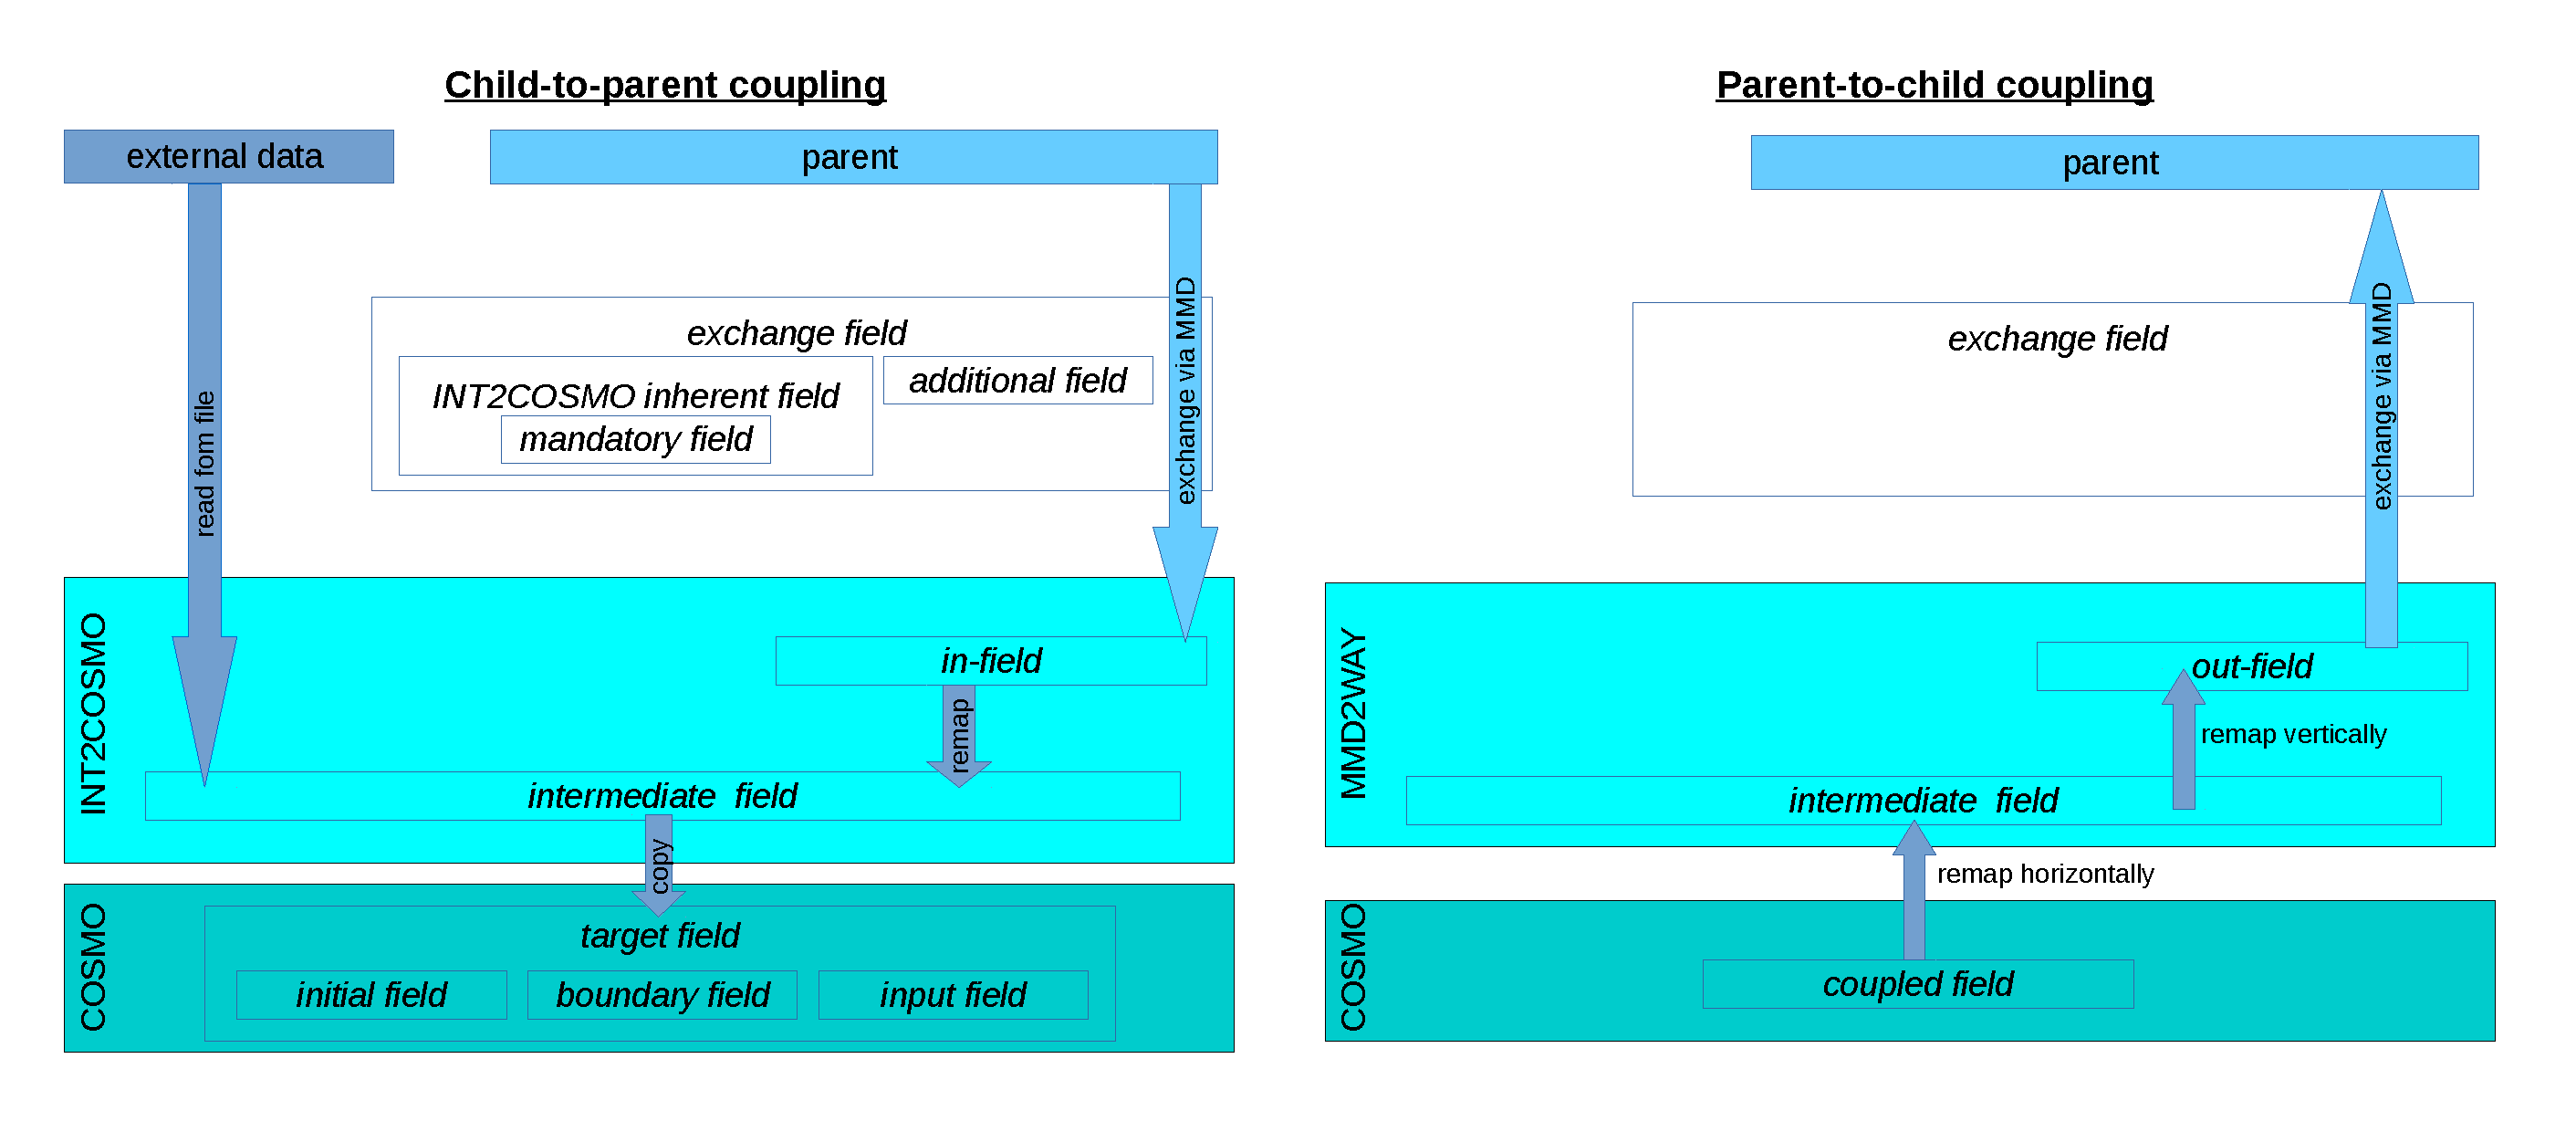
\includegraphics[width=0.9\textheight,angle=90]{MMDUM_fieldflow.pdf} 
\end{center} 
\vspace{-.8cm}
\caption{In the manual a lot of different specifications (all listed
in the glossary) are used. {\it Coupling fields} are all fields
somehow onvolved in the coupling procedure. The picture illustrates
the different stages and the meaning of the specific fields.}
\label{fig:fields} 
\end{figure*} 
%%%%%%%%%%%%%%%%

\end{appendix}

%+++++++++++++++++++++++++++++++++++++++++++++++++++++++++++++++++++++++++++
%+++++++++++++++++++++++++++++++++++++++++++++++++++++++++++++++++++++++++++
%+++++++++++++++++++++++++++++++++++++++++++++++++++++++++++++++++++++++++++
\clearpage

\bibliographystyle{copernicus} % bst file
\bibliography{MMDUM.bib}       % bib files

\end{document}
